



\documentclass[bibliography=totoc,listof=totoc,BCOR=5mm,DIV=12,oneside]{scrbook}
\usepackage[utf8]{inputenc}
\usepackage[T1]{fontenc}

\usepackage{lmodern}
\usepackage[ngerman]{babel}
\usepackage{microtype}
\usepackage{pifont}
\usepackage{amsmath}
\usepackage{hyperref}
\usepackage{booktabs} 
\usepackage{subfigure} 
\usepackage{colortbl}
\usepackage{pdfpages}
\usepackage{graphicx}
\usepackage{enumitem}
\usepackage{threeparttable}
\usepackage{float}
\usepackage{multirow}
\usepackage{listings}
\usepackage{color}

\definecolor{dkgreen}{rgb}{0,0.6,0}
\definecolor{gray}{rgb}{0.5,0.5,0.5}
\definecolor{mauve}{rgb}{0.58,0,0.82}

\lstset{frame=tb,
  language=Java,
  aboveskip=3mm,
  belowskip=3mm,
  showstringspaces=false,
  columns=flexible,
  basicstyle={\small\ttfamily},
  numbers=left,
  numberstyle=\tiny\color{gray},
  keywordstyle=\color{blue},
  commentstyle=\color{dkgreen},
  stringstyle=\color{mauve},
  escapeinside={(*@}{@*)},
  breaklines=true,
  breakatwhitespace=true,
  tabsize=3
}

\usepackage{pdflscape}
%\usepackage{lscape}
\setlength{\parindent}{0em} 
\usepackage[citestyle=numeric,natbib=true,style=numeric,backend=bibtex]{biblatex}
\usepackage{tabularx}

\newcommand*\adjust{\setlength\hsize{3\hsize+4\tabcolsep}} 

\addbibresource{lit.bib} 

\begin{document}

\frontmatter
    \pagestyle{empty}
\thispagestyle{empty}

\begin{center}

\vspace*{-2cm}


\includegraphics[width=1.2\textwidth]{Bilder/Form/fhl_logo.png}

\vspace*{3cm}
{\Large \textbf{Bachelorarbeit}}\\

\vspace{2.0cm}
{\Huge \textbf{Eine gamifizierte Howto-App für Bachelorarbeiten}}\\
\vspace*{3mm}

\vspace{1.5cm}

vorgelegt von
\vspace{1.5cm}

{\LARGE Tim-Pascal Lau} % Name des Autors
\vspace{2cm}

\parbox{1cm}{
\begin{large}
\begin{tabbing}
Ausgabedatum: \hspace{.5cm} \=24. Mai 2018\\
Abgabedatum: \>24. August 2018\\
\end{tabbing}
\end{large}}\\
\vspace{5mm}
\end{center}

\newpage
\chapter*{Aufgabenstellung}
\par Für Studierende im letzten Semester eines Bachelorstudiengangs umfasst \textbf{DIE} wesentliche Prüfungsleistung das Verfassen einer Bachelorarbeit.
Die Auseinandersetzung mit komplexen Problemstellungen stellt jedoch erfahrungsgemäß für viele Studierende eine große Herausforderung dar, welche sich aus dem erstmaligen Zusammenspiel von selbständigem und eigenverantwortlichem Arbeiten sowie Problemlösen mittels erworbener Fach- und Methodenkenntnisse über einen längeren (dreimonatigen) Zeitraum ergibt.

\par \bigskip Im Verlauf des Studiums sollten Studierende folgendes Wissen und folgende Fähigkeiten erworben haben und zielgerichtet anwenden können:
\begin{itemize}
\item Studiengang-spezifisches Grundlagenwissen
\item Wissensansammlung über fachspezifische Methoden und deren Eigenschaften
\item Die Fähigkeit, komplexe Probleme zu erkennen, zu strukturieren und systematisch mittels geeigneter Methoden zu bearbeiten
\end{itemize}

\par Es kommt im Kontext von Bachelorarbeiten dennoch oftmals zu Schwierigkeiten, das erworbene Wissen und Fähigkeiten zielgerichtet auf reale Probleme anzuwenden und deren Ergebnisse zusammenhängend zu dokumentieren.

\section*{Lösungsansatz}
\par Ein möglicher Lösungsansatz wäre es, Studierenden eine Software bereitzustellen, welche unterstützend und wegweisend bei dem systematischen Vorgehen für komplexe Problemstellungen fungieren könnte. Hierbei soll es nicht darum gehen, dem Studierenden die eigentliche Arbeit abzunehmen, sondern vielmehr darum, Studierende hinsichtlich Vorgehen und Methodenauswahl zielgerichtet zu unterstützen.
\par \bigskip Im Rahmen dieser Bachelorarbeit soll hierzu eine mobile Applikation entwickelt werden, die den Studierenden während der Dauer seiner Bachelorarbeit kontinuierlich \grqq begleitet\grqq. Dabei sollen Gamificationansätze realisiert werden, die motivierend im Rahmen einer Bachelorarbeit wirken sollen. Dies soll beispielhaft für den Studiengang Informatik/Softwareentwicklung erfolgen. Eine Erweiterbarkeit für andere Studiengänge ist hierbei jedoch von Anfang an konzeptionell vorzusehen.

\newpage
\par \bigskip Primäre Funktion der Software ist Studierenden bei den folgenden Aufgaben begleitend zu unterstützen und fortwährend zu motivieren \grqq am Ball zu bleiben\grqq:

\begin{itemize}
\item Brainstorming (zur Unterstützung der Ideenfindung für Bachelorarbeiten)
\item Recherche und Literaturverwaltung
\item Gliederung (unterschiedlicher Kategorien von Bachelorarbeiten, zum Beispiel mittels bewehrter Templates)
\item Zeitplanung/Fortschrittsverfolgung sowie Erinnerungs- und Benachrichtigungsfunktion 
\item Problem-orientierte Anforderungsanalyse und deren Dokumentation
\item Problem-orientierte Methoden- und Tool-/Framework-Selektion und deren Dokumentation
\item Methoden-spezifische Aufbereitung von Ergebnissen
\item Problem-orientierte Nachweisführung und deren Dokumentation
\end{itemize}
\par Die App soll mit Flutter für Android und iOS entwickelt werden. Dabei soll erhoben werden, inwiefern sich Flutter für die Entwicklung solcher Apps eignet (Lessons Learned).

\section*{Teilaufgaben}
\begin{itemize}
\item Detaillierte Anforderungsanalyse oben angegebener Funktionen. Hierbei sind Studenten und Professoren des Studiengangs Informatik/Softwaretechnik geeignet einzubeziehen und relevante Literatur (insbesondere zu Gamification und Methoden der Informatik und des Softwareengineering) zu berücksichtigen.
\item Architekturentwurf der Anwendung (Erweiterbarkeit für andere Studiengänge ist konzeptionell vorzusehen)
\item Implementierung der Anwendung
\item Die Funktionsfähigkeit der App soll mittels Softwaretests geeignet nachgewiesen werden.
\item Die Nutzbarkeit der App soll systematisch evaluiert werden. Hierbei sind Studenten und Professoren des Studiengangs Informatik/Softwaretechnik geeignet einzubeziehen.
\item Dokumentation der oben angegebenen Schritte inklusive Bewertung der Nutzbarkeit des Frameworks Flutter für solche Arten von Apps.
\end{itemize}

Es wird empfohlen die Dokumentation von Anfang an begleitend zur Arbeit zu erstellen und sich an einem Dokumentations-Template - wie bspw. diesem - zu orientieren.

\newpage

\includepdf[pages=-]{Bilder/Form/erklaerung.pdf}

\tableofcontents
\newpage
\mainmatter
\pagestyle{plain}

\chapter{Einleitung}
\par Für Studierende im letzten Semester eines Bachelorstudiengangs umfasst die wesentliche Prüfungsleistung das Verfassen einer Bachelorarbeit.
Die Auseinandersetzung mit komplexen Problemstellungen stellt jedoch erfahrungsgemäß für viele Studierende eine große Herausforderung dar, welche sich aus dem erstmaligen Zusammenspiel von selbständigem und eigenverantwortlichem Arbeiten sowie Problemlösen mittels erworbener Fach- und Methodenkenntnisse über einen längeren (dreimonatigen) Zeitraum ergibt.

\section{Motivation}
\par Im Verlauf des Studiums sollten Studierende folgendes Wissen und folgende Fähigkeiten erworben haben und zielgerichtet anwenden können:
\begin{itemize}
\item Studiengang-spezifisches Grundlagenwissen
\item Wissensansammlung über fachspezifische Methoden und deren Eigenschaften
\item Die Fähigkeit, komplexe Probleme zu erkennen, zu strukturieren und systematisch mittels geeigneter Methoden zu bearbeiten
\end{itemize}

\par \bigskip Des Weiteren stellt eine Online-Umfrage den Teil der Datenerhebung dar, die quantitative Ergebnisse erzielt und deren Aussage somit eine nicht durch die schriftlichen Befragungen abgebildete Menge darstellt.
\par Die Umfrage richtete sich nicht nur an die Studierenden des Studiengangs Informatik/Softwaretechnik, sondern an Studierende im Allgemeinen, welche sich ab dem 4. Semester bereits in der zweiten Hälfte des Studiums befinden und somit schon einen einschätzbaren Erfahrungsschatz aufgebaut haben. Diese Umfrage fließt jedoch nicht mit in die Anforderungsanalyse ein, sondern dient lediglich dazu, ein allgemeines Bild des Bedarfs der zu entwickelnden Software zu ermitteln.

\newpage
\subsection{Voruntersuchung zur Ermittlung der Bedarfssituation}
\par \bigskip Im Vorfeld zur Entwicklung der Applikation wurde eine Online-Umfrage an verschiedenen Hochschulen durchgeführt (siehe Anhang \ref{anhang:onlineUmfrageStudierendeErgebnisse}), welche als Voruntersuchung des Problemfeldes dient und somit einen ersten Eindruck über den Bedarf an einer Software zur Unterstützung der Studierenden bei der Bearbeitung der Bachelorarbeit liefert.

\par \bigskip Insgesamt haben 44 Studierende unterschiedlicher Hochschulen an der Umfrage teilgenommen, wobei sich diese in weitere drei Gruppen aufteilen lassen. Diese Unterteilung erfolgt nach den unterschiedlichen Phasen, in denen sich die jeweiligen teilnehmenden Studierenden zur Zeit der Umfrage befinden. 

\par \bigskip Im Folgenden werden die wichtigsten Erkenntnisse der zusammengefassten Umfrage (siehe Abbildung \ref{img:zusammenfassungOnlineUmfrage}) beschrieben:

\begin{itemize}
\item \textbf{Vor Beginn der Bachelorarbeit (Ab 4. Semester)}
\par \textbf{Teilnehmerzahl: 24}
\par Die Ergebnisse der Befragung von Studierenden, die sich noch vor der Bearbeitung der Bachelorarbeit befinden, zeigen bezüglich der Kenntnisse über Ablauf der Bachelorarbeit und Erwartungen an den Studierenden, sowie deren Einschätzung zu Selbst- und Zeitmanagement ein relativ gleichmäßig verteiltes Bild der Situation auf. 
\par Hierbei fällt auf, dass ein nicht geringer Teil explizit angibt, Schwierigkeiten mit den genannten Aspekten zu haben. 

\item \textbf{Während der Bachelorarbeit}
\par \textbf{Teilnehmerzahl: 14}
\par Bei Betrachtung der Umfrageergebnisse der Studierenden, die sich in der Phase während der Bachelorarbeit befinden, ist abzulesen, dass es im Kontext von Bachelorarbeiten unter einem nicht geringen Teil der Studierenden zu Schwierigkeiten kommt. 
\par Hierbei gelten besonders das Zeitmanagement und das wissenschaftliche Arbeiten durchaus als problematisch. Weiterhin sagt über die Hälfte der Studierenden aus, dass sie mit der gesamten Bearbeitung der Bachelorarbeit überfordert sind und ein weiterer Teil, dass sie sich nicht ausreichend mit den Formalien einer Bachelorarbeit auskennen. Viele der Studierende fühlen sich unsicher gegenüber dem, was von ihnen erwartet wird, schätzen sich im Allgemeinen jedoch durch das Studium, als gut vorbereitet ein.

\item \textbf{Nach Abschluss der Bachelorarbeit}
\par \textbf{Teilnehmerzahl: 6}
\par Auffällig einstimmig verhalten sich die Ergebnisse der Studierenden, die sich bereits nach Abschluss der Bachelorarbeit befinden. Das selbstständige Arbeiten sowie das Einschätzen von Zeitaufwand haben nach Aussage der Studierenden offensichtlich wenig bis keine Schwierigkeiten dargestellt. Weiterhin geben die Befragten an, sich bei der Fertigstellung der Bachelorarbeit nicht überfordert gefühlt zu haben. Ein wichtiges Detail ist jedoch, dass über die Hälfte der Befragten angeben, sich durch das Studium nicht ausreichend auf die Bachelorarbeit vorbereitet gefühlt zu haben. 
\end{itemize}

\bigskip
\begin{figure}[H]

	\subfigure[Vor Beginn der Bachelorarbeit]
	{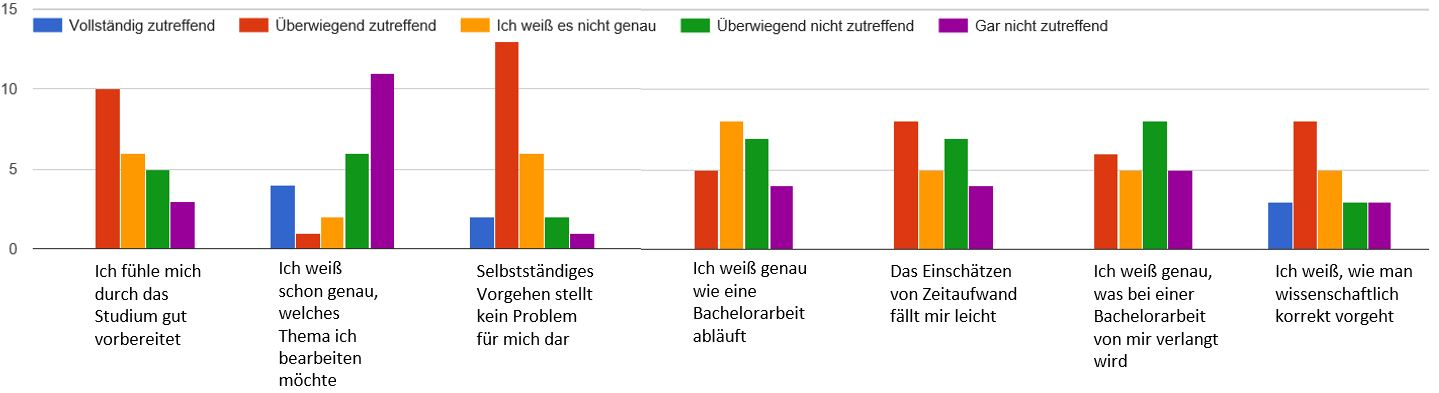
\includegraphics[width=1\textwidth, keepaspectratio]{Bilder/ZusammenfassungVorBachelorarbeit.JPG}}
	
	\vspace{1.5cm}
	\subfigure[Während der Bachelorarbeit]
	{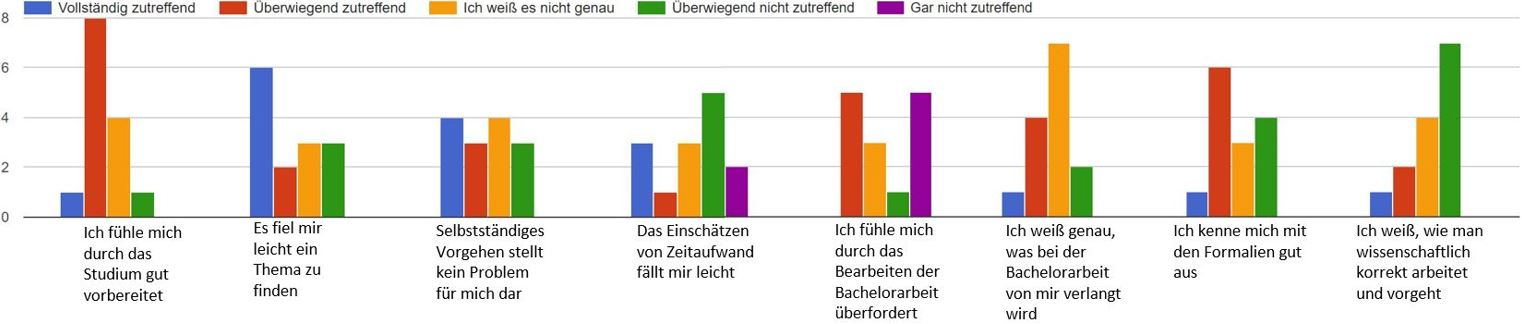
\includegraphics[width=1\textwidth, keepaspectratio]{Bilder/ZusammenfassungWaehrendBachelorarbeit.JPG}}
	
	\vspace{1.5cm}
	\subfigure[Nach Abschluss der Bachelorarbeit]
	{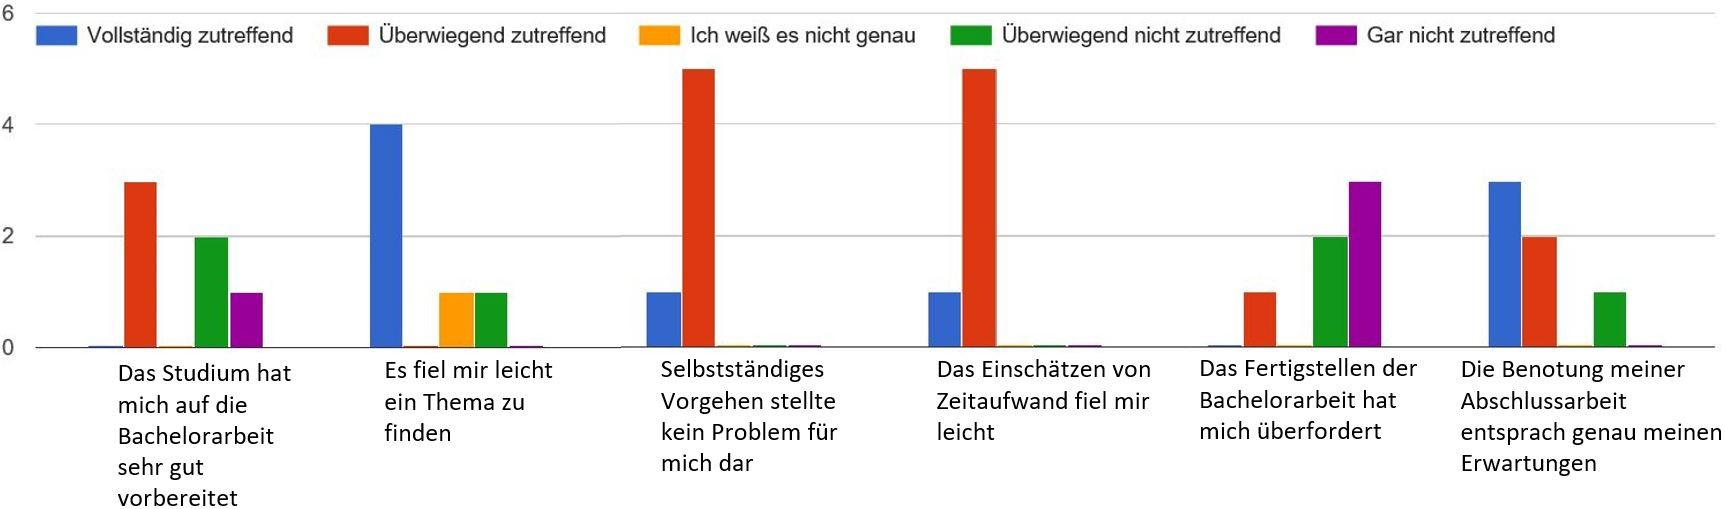
\includegraphics[width=1\textwidth, keepaspectratio]{Bilder/ZusammenfassungNachBachelorarbeit.JPG}}
	
	\caption{Online Umfrage: Zusammenfassung der Umfrageergebnisse}
	\label{img:zusammenfassungOnlineUmfrage}
\end{figure}

\par \bigskip Das Gesamtbild der Umfrage zeigt die verschiedenen Schwierigkeiten, mit denen Studierende im Laufe der Bachelorarbeit zu tun haben und stellt diese als wichtige Untersuchungselemente zur Analyse des Problembereichs heraus.

\section{Lösungsansatz und Zielstellung}
\par Ein möglicher zu verfolgender Lösungsansatz wäre es, eine Software zu entwickeln, welche unterstützend und wegweisend bei dem systematischen Vorgehen unter komplexen Problemstellungen fungieren könnte und auf diese Weise dabei hilft, den Ablauf der Bachelorarbeit für Studierende zugänglicher zu gestalten.
\par Hierbei soll es nicht darum gehen, den Studierenden die eigentliche Arbeit abzunehmen, sondern vielmehr darum, Studierende hinsichtlich Vorgehen und Methodenauswahl zielgerichtet zu unterstützen.

\par \bigskip Mit einem solchen Ansatz soll es Studierenden ermöglicht werden, ihr gelerntes Wissen durch Fokussierung bestimmter Aufgaben und Zusammenhänge im Rahmen ihres eigenen Bachelorprojekts auf die Realität zu übertragen und somit einen motivierenden sowie weiterhin fordernden Rahmen zu schaffen, um ihr Bachelorprojekt erfolgreich abzuschließen.

\section{Aufgabenbeschreibung}
Im Rahmen dieser Bachelorarbeit soll hierfür eine mobile Applikation entwickelt werden, die den Studierenden während der Dauer der Bachelorarbeit kontinuierlich \grqq begleitet\grqq . Dabei sollen Gamificationansätze realisiert werden, welche motivierend bei der Bearbeitung und dem Vorgehen bei der eigenen Bachelorarbeit wirken sollen. Dies soll beispielhaft für den Studiengang Informatik/Softwareentwicklung erfolgen. Eine Erweiterbarkeit für andere Studiengänge ist hierbei jedoch konzeptionell vorzusehen.
Primäre Funktion der Software ist, Studierenden bei den folgenden Aufgaben begleitend zu unterstützen und fortwährend zu motivieren \grqq am Ball zu bleiben\grqq:
\begin{itemize}
\item Brainstorming (zur Unterstützung der Ideenfindung für Bachelorarbeiten)
\item Recherche und Literaturverwaltung
\item Gliederung (unterschiedlicher Kategorien von Bachelorarbeiten, zum Beispiel mittels bewehrter Templates)
\item Zeitplanung/Fortschrittsverfolgung sowie Erinnerungs- und Benachrichtigungsfunktion 
\item Problem-orientierte Anforderungsanalyse und deren Dokumentation
\item Problem-orientierte Methoden- und Tool-/Framework-Selektion und deren Dokumentation
\item Methoden-spezifische Aufbereitung von Ergebnissen
\item Problem-orientierte Nachweisführung und deren Dokumentation
\end{itemize}
Die Applikation soll mittels Flutter für Android und iOS entwickelt werden. Dabei soll erhoben werden, inwiefern sich Flutter für die Entwicklung solcher Apps eignet(Lessons Learned). 

\par Die im Rahmen der Aufgabenbeschreibung entstandenen Anforderungen werden durch die folgenden Teilaufgaben spezifiziert:
\begin{itemize}
\item Detaillierte Anforderungsanalyse oben angegebener Funktionen. Hierbei sind Studenten und Professoren des Studiengangs Informatik/Softwaretechnik geeignet einzubeziehen und relevante Literatur (insbesondere zu Gamification und Methoden der Informatik und des Softwareengineering) zu berücksichtigen.
\item Architekturentwurf der Anwendung (Erweiterbarkeit für andere Studiengänge ist konzeptionell vorzusehen)
\item Implementierung der Anwendung
\item Die Funktionsfähigkeit der App soll mittels Softwaretests geeignet nachgewiesen werden.
\item Die Nutzbarkeit der App soll systematisch evaluiert werden. Hierbei sind Studenten und Professoren des Studiengangs Informatik/Softwaretechnik geeignet einzubeziehen.
\item Dokumentation der oben angegebenen Schritte inklusive Bewertung der Nutzbarkeit des Frameworks Flutter für solche Arten von Apps.
\end{itemize}

\newpage
\section{Ausblick auf die Bachelorarbeit}
\par In der folgenden Dokumentation der Bachelorarbeit sind verschiedene aufeinander aufbauende Prozesse, Teilschritte und Ergebnisse der Softwareentwicklung dokumentiert. 

\par \bigskip Im Rahmen dieses Projekts werden verschiedene Inhalte aus dem Gebiet der Gamification bezüglich Software-Anwendungen behandelt. Um einen Eindruck über die Umsetzung und Bedeutung von gamifizierten Inhalten in modernen Software-Anwendungen zu bekommen, werden im \textbf{Kapitel \ref{chap:grundlagenkapitel}}, die für diese Arbeit benötigten Grundlagen beschrieben.
\par Weiterhin enthält das Grundlagenkapitel wichtige Informationen für die Nachvollziehbarkeit der für die Entwicklung der Software gewählten Redux-Architektur unter Verwendung von Google's Framework Flutter und dessen Funktionsweise.

\par \bigskip Das Durchführen der Anforderungsanalyse im Rahmen einer Softwareentwicklung, ist je nach Ausgangspunkt mit einem enormen Aufwand verbunden, da je nach Komplexität viele verschiedene Personen in ein ihnen fremdes Projekt einbezogen werden. Im Rahmen diese Projekts haben sich sowohl Professoren der Fachhochschule Lübeck als auch Studierende bereit erklärt, an Interviews und weiteren Einbindungen in das Projekt teilzunehmen und somit das zu untersuchende Problemfeld schrittweise aufzudecken. Die aus der gewählten Befragungsstrategie resultierenden Ergebnisse werden im \textbf{Kapitel \ref{chap:problemanalyse}} diskutiert und durch das Ableiten von präzisen Lösungsmöglichkeiten beschrieben.

\par \bigskip Basierend auf den abgeleiteten Anforderungen, werden im folgenden Verlauf der Dokumentation die verschiedenen Abstraktionsebenen der Software beschrieben. In \textbf{Kapitel \ref{chap:konzept}} wird anhand der Oberfläche der Applikation das Gesamtkonzept unter Einbezug von Hintergründen der gewählten Lösungswege und Designentscheidungen beschrieben, wohingegen in Kapitel \ref{chap:architektur} die Beschreibung der wichtigsten Details zur technischen Umsetzung der Softwarelösung ausgeführt wird.

\par \bigskip Nach der Entwicklung einer Softwarelösung sollte letztendlich immer der wichtige Schritt der Evaluation folgen, welcher in diesem Fall erneut durch das Einbeziehen von Professoren und Studierenden stattfinden konnte. Die Ergebnisse dieser Evaluation, der Softwaretest und die abschließende Bewertung des Frameworks Flutter werden im \textbf{Kapitel \ref{chap:nachweisführung}} behandelt.

\par \bigskip Jeder dieser beschriebenen Kapitel trägt im Kern die Schwerpunkte einer jeden Softwareentwicklung, welche sich zwischen technischem Fachwissen und Kompetenzen (Hard Skills) und der zwischenmenschlichen Kommunikationsfähigkeit sowie der eigenen Persönlichkeit (Soft Skills) definieren lassen. Nach Durchführung des Projekts wurden durch alle einzelnen Schritte Teil- sowie Gesamtergebnisse erreicht, welche im abschließenden \textbf{Kapitel \ref{chap:ergebnisse}} zusammenlaufen und unter Schilderung eigener Erfahrungen diskutiert werden sowie einen Ausblick auf die Zukunft des Projekt ermöglichen.

\chapter{Beschreibung der Kernkomponenten} 
\par In diesem Kapitel werden die Grundlagen zur Nachvollziehbarkeit dieser Projektarbeit vermittelt. Es wird somit empfohlen die folgenden Kapitel zu Gamification, Flutter und die für die Beschreibung der Implementierungsdetails relevanten Redux-Architektur zu lesen, um ein Gesamtverständnis für Begriffe und weitere Zusammenhänge des Projekts zu ermöglichen.

\label{chap:grundlagenkapitel}
\section{Gamification} 
\label{sec:grundlagenkapitelGamification}
\par Im folgenden Kapitel werden die für diese Arbeit relevante Informationen bezüglich Gamification vermittelt. Hierbei wird erst auf die grundlegende Bedeutung sowie deren Abgrenzung gegenüber verschiedenen Ansätzen eingegangen. Im weiteren Verlauf werden dann tiefgreifendere Informationen zu den verschiedenen Benutzerklassen und den jeweiligen kompatiblen Spiel-Design-Elementen beschrieben.

\subsection{Die Bedeutung von Gamification}
\par Im Kontext dieser Ausarbeitung wird sich auf die in \citep{deterding2011gamification} genannte Definition für den Begriff \grqq Gamification\grqq{} bezogen:
\begin{quotation} 
Gamification is the use of elements of game design in non-game contexts. 
\end{quotation}
\par Was sich aus dieser Definition ableiten lässt, beschreibt  Gamification als das Einsetzen spieltypischer Elemente in einem spielfremden Kontext.
\par Somit lässt sich ein Kontext bereits als \grqq gamifiziert\grqq{}
beschreiben, sobald Spiel-Design-Elemente in den spezifischen Kontext integriert worden sind, weshalb besonders im Rahmen der Unternehmenseinführung von Gamification-Ansätzen zwischen \textbf{Enterprise Gamification} und \textbf{Serious Games} unterschieden wird\citep[vgl. Kapitel 1.1 Gamification: Definition und Abgrenzung, Seite 4]{Sailer2016}.
\par \bigskip \textbf{Enterprise Gamification} bezeichnet das konkrete Einbinden von Gamification-Elementen in Arbeits- und/oder Lernprozessen, mit dem expliziten Ziel der Motivationssteigerung seitens der Anwender.
\par \bigskip Gegenüber diesem Ansatz hat sich weiterhin der Begriff \textbf{Serious Games} integriert, welcher das explizite Einsetzen von Spielen in einem ernsten Kontext vorsieht und die Unterhaltung nicht im Fokus der Anwendung steht, sondern die Wertschöpfung von Wissen und Realwelterfahrungen. 

\newpage
\subsection{Bekannte Spiel-Design-Elemente} \label{sub:grundlagenSpielDesignElemente}

\par Im folgenden Kapitel werden die wichtigsten interaktiven Spiel-Design-Elemente, welche in Tabelle \ref{tab:spielDesignElemente} genannt werden, vorgestellt und beschrieben. 
\par Der Einsatz von Gamification-Elementen basiert auf der Annahme, dass diese die grundsätzlichen Bedürfnisse der Menschen ansprechen (vgl. \citep[Kapitel 1.1 Enterprise Gamification - Vorgehen und Anwendung, Seite 5]{Sailer2016}).

\bigskip
\begin{tabularx}{\textwidth}{X|l|l}
	\toprule
	\textbf{Spiel-Mechanik} & \textbf{Spiel-Dynamik} & \textbf{Motiv}\\ \midrule
	Dokumentation von Verhaltensweisen & Exploration & Wissbegierde\\
	Punktesysteme, Badges, Trophäen & Sammeln  & Leistung\\
	Ranglisten & Wettbewerb & Soziale Anerkennung\\ 
	Ränge, Levels, Reputationspunkte & Statuserwerb  & \\
	Gruppenaufgaben & Zusammenarbeit  & Sozialer Austausch\\
	Zeitdruck, Aufgaben, Missionen & Herausforderung & Kognitive Stimulation\\ 
	Avatare, virtuelle Welten, virtueller Handel & Entwickeln/Organisieren & Selbstbestimmung \\ 
	\bottomrule
\end{tabularx}
\captionof{table}{Übersicht der Spiel-Design-Elemente \citep[vgl.]{blohm2013gamification}}
\label{tab:spielDesignElemente}

\par \bigskip Die folgenden aufgeführten Informationen wurden größtenteils aus den Werken \citep[Kapitel 2.2.2 Analyse einzelner Spiel-Design-Elemente]{Sailer2016} und \citep[Kapitel 4 The Gamification Toolkit Game Elements]{werbach2012win} entnommen, bei Abweichungen werden die konkreten Literaturwerke aus Gründen des Leseflusses explizit angegeben.

\par \bigskip \textbf{Dokumentation von Verhaltensweisen}
\par Durch die ständige Dokumentation der eigenen Verhaltensweisen, werden persönliche Fortschritte für den Anwender sichtbar gemacht. Diese Fortschritte können ein Gefühl von hoher Leistungsfähigkeit auslösen, da auf diese Weise ein Vergleich zu den bisherigen erreichten Leistungen ermöglicht wird und somit bei Verbesserung der eigenen Leistung der persönliche Fortschritt verdeutlicht werden kann.

\par \bigskip \textbf{Punkte}
\par Punktesysteme sind in ihrer Einfachheit eine weitverbreitete Form der Spiel-Design-Elemente, welche hauptsächlich eine Feedback-Funktion erfüllen. Diese Feedback-Funktion kann dem Spieler durch diverse weitere Möglichkeiten, wie zum Beispiel durch das Aufsteigen eines Levels, unterschiedlich stark verdeutlicht werden, weshalb Punkte häufig als Grundbestandteil von Gamification-Anwendungen auftreten. Weiterhin symbolisieren Punkte dem Spieler seinen derzeitigen Spielstand und bieten bei der Kombination mit Bestenlisten eine Vergleichsmöglichkeit zu anderen Spielern. In dieser Kombination können Punktesysteme also je nach Zielstellung auch Gewinner einer Herausforderung identifizieren.
\par In den zwei, in \citep{Sailer2016} behandelten, empirischen Untersuchungen \citep{mekler2013disassembling} und \citep{mekler2013points}, wurde nachgewiesen, dass der Einsatz von Punktesystemen durchaus einen leistungsfördernden Effekt auf die Spieler haben kann.

\newpage
\par \bigskip \textbf{Abzeichen}
\par Die Abzeichen, welche sich in der Regel durch erreichbare Achievements, Badges und/oder Trophäen innerhalb von Gamification-Anwendungen etabliert haben, dienen einerseits einer zielsetzenden und darüber Hinaus auch einer nicht-kontrollierenden Feedback-Funktion. 
\par Zu erwähnen gilt, dass Badges und Trophäen nicht mit Achievements gleichzusetzen sind, sondern lediglich die visuelle Repräsentation eines Achievements darstellen.
\par Durch den Einsatz solcher Spiel-Design-Elemente soll der Benutzer sinnvoll gefordert werden und sich im Optimalfall durch das somit klar gesteckte Ziel motiviert fühlen.
\par \medskip Weiterhin lassen sich bei dem Einsatz von Achievements unterschiedliche strategische Ansätze identifizieren, die sich von der bereits genannten zielsetzenden Strategie abheben. 
\par Beispielsweise kann bewusst auf die Angabe des Ziels eines Achievements verzichtet werden, um je nach Kontext die Neugierde des Benutzers zu fördern und den Effekt des Erreichens umso größer ausfallen zu lassen, da diese Achievements durch Ausführen verschiedener Tätigkeiten überraschend erreicht werden. Dies spricht aufgrund des erforschenden Charakters vor allem die Benutzerklasse \textbf{Explorer} an (siehe Kapitel \ref{sub:nutzergruppenBartle}). 
\par \bigskip Auf diese Weise kann auch eine stärkere Bindung einer Comunity entstehen, da der Austausch zwischen Benutzern, die bereits wissen wie ein bestimmtes Achievement erreicht wird und denjenigen, die es noch nicht erreicht haben, die Kommunikation untereinander fördern kann.

\par \bigskip \textbf{Ranglisten}
\par Die sogenannten Rang- oder auch Bestenlisten dienen der Identifikation und Abgrenzung von unterschiedlichen Benutzern, die im Kontext der Gamification-Anwendung unterschiedliche Erfolge, häufig in Form von Punkten, erreicht haben.
\par Zentrale Absicht solcher Ranglisten ist das Darstellen der besten Spieler, was je nach Kontext für einen hohen kompetitiven Anwendungsanteil spricht.

\par \medskip Im Rahmen von Ranglisten-Spiel-Elementen können weiterhin verschiedene Kategorien identifiziert werden, welche sich auf unterschiedliche Weise durch verschiedene Vor- und Nachteile des jeweiligen Zielkontextes äußern.
\par Während individuelle Ranglisten die Leistung des Einzelnen aufzeigen und somit versuchen das Individuum von den restlichen Spielern abzugrenzen, ermöglichen team-basierte Ranglisten das kooperative Vernetzen unterschiedlicher Personen und Identifizieren ganzer Team-Leistungen.


\par \bigskip \textbf{Ränge, Level und Reputationspunkte}
\par Wie in \citep[Kapitel 4.5 Reputations, Ranks and Levels, Seite 75]{reeves2009total} beschrieben wird, können Reputationsmöglichkeiten für Benutzer ein wichtiges Identifikationsmittel sein. Durch die Möglichkeit bestimmte Ränge oder Level zu erreichen, sind Spieler besonders im Rahmen von Multiplayer-Anwendungen dazu angehalten, ihr Ansehen gegenüber anderen Spielern zu steigern oder zu festigen und somit den Status eines Veteranen zu repräsentieren.
\par Diese Art von Spiel-Elementen ermöglicht das Ausstrahlen von Kompetenzen, Talenten sowie Erfahrungen und somit den Platz, den der jeweilige Spieler in der Spielwelt einnimmt.

\par \bigskip \textbf{Avatare, virtuelle Welten, virtueller Handel}
\par Durch die Möglichkeit der Erstellung eines persönlichen Avatars werden dem Spieler je nach Ausprägung hoch oder gering ausfallende Individualisierungs- und somit auch Identifikationsmöglichkeiten angeboten. 
\par Ein wichtiger Aspekt, welcher je nach Anwendungsfeld unterschiedlich ausgelegt wird, ist das Interagieren mit der virtuellen Welt, in der sich der Avatar befindet. Hierbei kann es zur Interaktion mit anderen Spieler-Avataren oder mit definierten Teilen der virtuellen Welt kommen. Die virtuelle Welt kann hierbei beispielsweise Möglichkeiten bieten, sich frei in einer dreidimensionalen Umgebung zu bewegen. 
\par Die virtuelle Welt muss nicht zwangsweise dreidimensional ausfallen, sondern kann durch geschickte Konzipierung des Interface-Designs auch mit weniger Umgebungsfreiheit den gewünschten Effekt erzielen.

\par \bigskip \textbf{Zeitdruck, Aufgaben, Missionen}
\par In \citep[Kapitel 6.1.1 Tasks]{pflanzl2018gamification} wird beschrieben, dass Aufgaben und Missionen im Kontext von Gamification-Anwendungen sehr breit vertretene Varianten von Spiel-Design-Elementen sind. 
\par Sie können sehr gut mit anderen Elementen wie Level-Systemen kombiniert werden und lassen sich durch die hohe Individualisierbarkeit der Aufgabeninhalte im Rahmen des jeweiligen Anwendungskontext als ziel- oder wegweisende Spiel-Elemente benutzen, die gleichzeitig in direkter Form auf das tatsächliche Anwendungsfeld Bezug nehmen.

\par \bigskip \textbf{Gruppenaufgaben}
\par Wie in \citep[Kapitel 6.1.1 Tasks]{pflanzl2018gamification} weiterhin beschrieben wird, stehen die Gruppenaufgaben, wie auch die Einzelaufgaben, für eine zu erfüllende Gesamtaufgabe. Eine Gruppenaufgabe hebt sich jedoch insofern ab, dass sie aus mehreren kleinen Aufgaben besteht, welche im Team gelöst werden sollen. Wie auch in den Team-Bestenlisten rückt bei Einsatz dieser Elemente die kooperative Ausführung von Aufgaben in den Vordergrund und soll so durch eine starke Teamidentifikation für eine erhöhte Motivation des Einzelnen sorgen.

\subsection{Nutzergruppen nach Bartle} \label{sub:nutzergruppenBartle}
\par Nach Bartle \citep{bartle1996hearts} werden vier verschiedene Nutzertypen voneinander unterschieden, welche in vielen Literaturwerken zur Gamification als Grundlage oder zumindest als Orientierung referenziert werden.
 
\par Die vier verschiedenen Nutzerklassen werden im folgenden Verlauf vorgestellt und hinsichtlich ihrer Bedürfnisse erläutert:
\begin{itemize}
\item \textbf{Der Killer}
\par Die Killer legen den Fokus auf den Wettkampf. Somit beruht ihre Motivationsquelle auf stark kompetitiv ausgeprägte Ansätze. Sie fühlen sich dadurch motiviert, den Kontakt mit anderen Individuen im Rahmen eines Wettkampfes zu suchen und sich durch den eigenen Sieg gegenüber anderen Personen zu behaupten.

\item \textbf{Der Socialiser}
\par Die Gruppe der Socialiser sind auf der Suche nach sozialer Interaktion. Ohne diese können sie der Spielwelt wenig bis keine Motivation abgewinnen. Die Spielwelt, in der sie sich bewegen, ist vor allem nur das Mittel zum Zweck der Kommunikation. Der größte Anreiz der Socialiser ist die Freundschaft und der Kontakt zu anderen Personen.

\newpage
\item \textbf{Der Achiever}
\par Die Achiever konzentrieren sich auf das Erbringen von Leistungen und das Abschließen von Herausforderungen. Sie werden so eingeschätzt, dass sie die möglichst optimale geforderte Leistung erbringen wollen und daher ihre Motivation aus dem schrittweisen Sammeln von Erfolgen und dem Erfüllen von Aufgaben ziehen.

\item \textbf{Der Explorer}
\par Die Explorer legen den Hauptfokus auf die Welt, in der sie sich bewegen und möchten im Zusammenspiel mit dieser Spielwelt durch immer wieder neu gestellte Aufgaben und erlebte Überraschungen alles entdecken, was es zu entdecken gibt. Sie sind sehr ambitioniert und empfinden Stolz für ihr Wissen und ihre Erfahrung in der Spielwelt. 
\par Die Explorer haben vor allem Interesse an der Spielwelt und weniger an den Personen, die sie im Laufe der Erkundung treffen.
\end{itemize}

\par \bigskip Wie aus den Beschreibungen zu erkennen ist, entsteht bei der allgemeinen Betrachtung aller Benutzerklassen ein Spannungsfeld der Interessen, welches in Abbildung \ref{img:interetGraphBartle} verdeutlicht werden soll.

\bigskip
\begin{figure}[H]
	\centering
	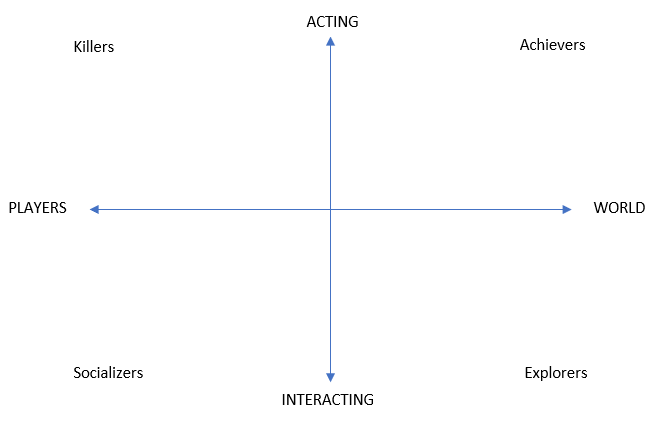
\includegraphics[width=0.75\textwidth, keepaspectratio]{Bilder/Diagramme/InterestGraphBartle.png}
	\caption{Interest Graph nach Bartle \cite{bartle1996hearts}}
	\label{img:interetGraphBartle}
\end{figure}

\par \bigskip Das Spannungsfeld wird weiterhin definiert durch die vier verschiedenen Interessenausprägungen der Spieler (Players), der virtuellen Welt (World), des Handelns in dieser Welt (Acting) und des Interagierens mit der virtuellen Welt (Interacting).

\newpage
\section{Vorstellung des Frameworks Flutter}
\par Flutter ist ein von Google entwickeltes Open-Source-Framework, das auf die Entwicklung mobiler 2D-Applikationen für Android- und iOS-Betriebssysteme ausgelegt ist. 
\par \medskip Beworben wird Flutter seit der Ankündigung der Beta-Version, welche in einem offiziellen Blogeintrag der \textbf{Google Developers}\citep{AnouncingFlutterBeta} im Rahmen des \textbf{Mobile World Congress 2018}\citep{MobileWordCongress} veröffentlicht wurde, unter anderem durch eine besonders flexibel handhabbare und mit Leichtigkeit umzusetzende Gestaltung von hochqualitativen Benutzeroberflächen. Weiterhin wird betont, dass die zu erzielenden Ergebnisse das Produkt einer extrem schnell umsetzbaren Entwicklung \grqq in Rekordzeit\grqq{} sind.

\par \medskip Im folgenden Kapitel werden die Kernprinzipien von Flutter erläutert und die framework-spezifischen Besonderheiten beschrieben um Ihnen als Leser einen Eindruck von dem Framework zu ermöglichen und die grundsätzliche Funktionsweise sowie dessen Besonderheiten, hinter den werbe-zweckmäßigen Worten der öffentlichen Präsentation, nachvollziehbar zu gestalten.

\subsection{Flutter Kerntechnologien} 
Das Flutter Framework besteht aus verschiedenen Basiskomponenten, welche aus aufeinander aufbauenden Systemschichten bestehen (siehe Abbildung \ref{img:flutterHighLevelSystemOverview}) und sich auf oberster Abstraktionsebene auf die Flutter-Engine und das Flutter-Framework unterteilen lassen.

\bigskip
\begin{figure}[H]
	\centering
	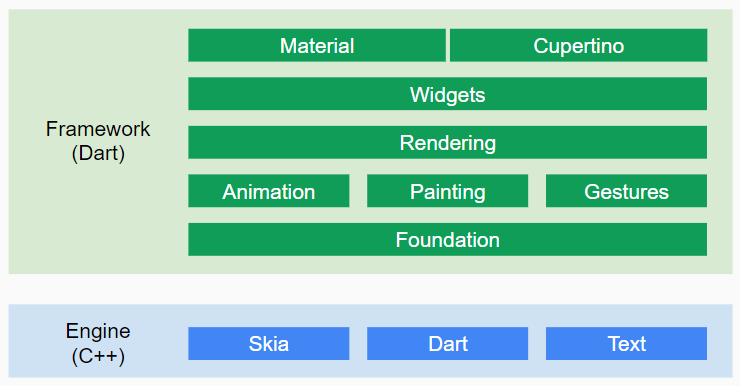
\includegraphics[width=0.8\textwidth, keepaspectratio]{Bilder/highLevelOverview.png}
	\caption{Flutter High-Level Systemarchitektur \cite{Flu5}}
	\label{img:flutterHighLevelSystemOverview}
\end{figure}

\par \bigskip Im folgenden Abschnitt werden die drei Basistechnologien von Flutter kurz beschrieben:

\par \bigskip \textbf{Flutter Engine}
\par Wie in dem Flutter Wiki \citep{Flu4} beschrieben wird, setzt sich die C/C++ basierte Flutter Engine aus den drei Kerntechnologien Skia\citep{Skia1}, eine open source 2D Graphics Libary, die Dart Virtual Machine sowie die verschiedenen verwendeten Bibliotheken zum Rendern von Texten zusammen.

\newpage
\par \bigskip \textbf{Foundation Libary}
\par Die Dart-basierte Foundation Libary\citep{FoundationLibary} stellt Basisklassen und -funktionen zur Verfügung, die von den anderen in der Flutter-Architektur überliegenden Schichten genutzt werden (siehe Abbildung \ref{img:flutterHighLevelSystemOverview}) und stellt somit eine zentralen Grundlage bei der Konstruktion von Applikationen mittels dem Flutter-Framework dar.

\par \bigskip \textbf{Design-specific Widgets}
\par Das Flutter-Framework stellt zwei verschiedene Design-Stile der Widgets zur Verfügung, welche den jeweiligen Design-Sprachen von \textbf{Google Material Design}\citep{Mat1}, welche 2014 entwickelt wurde sowie die \textbf{iOS Design}\citep{iOSDesign} kopierende Design-Sprache \textbf{Cupertino}\citep{Cup1} entsprechen.

\subsection{Plattformübergreifende Entwicklung von mobilen Applikationen}
\par Flutter ermöglicht das plattform-unabhängige Entwickeln von mobilen Applikationen für Android- und iOS-Betriebssysteme und verarbeitet oberflächen-spezifische Darstellungsformen der jeweiligen Zielplattformen framework-intern. Dies bedeutet, dass zum Zeitpunkt der Entwicklung auf extrem abstrakter Ebene ein Oberflächendesign unabhängig von der Zielplattform konzipiert werden kann, da die plattform-spezifischen Darstellungsweisen von dem Framework selbst gelöst werden und von den jeweiligen Entwicklern nicht berücksichtigt werden müssen. 
\par \bigskip \textit{Hinweis: Die in Abbildung \ref{img:FlutterVisualisierungiOSAndoid} gezeigten Oberflächen entstammen demselben Programmcode.}

\bigskip
\begin{figure}[H]
	\centering
	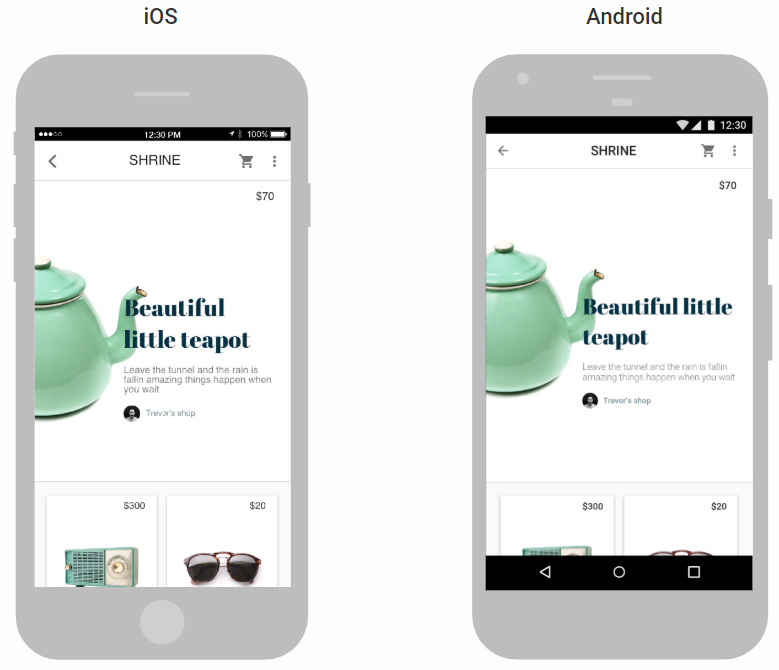
\includegraphics[width=0.55\textwidth, keepaspectratio]{Bilder/PlattformUebergreifendDesign.png}
	\caption{Darstellung (iOS und Android): Plattformunabhängige Entwicklung von Applikationen \cite[What is Flutter?]{Flu8}}
	\label{img:FlutterVisualisierungiOSAndoid}
\end{figure}

\newpage
\subsection{Hot-Reload Funktion}
\par Die sogenannte \grqq Hot Reload\grqq -Funktion spielt im Rahmen der App-Entwicklung mit Flutter eine primäre Rolle, da bei Änderungen an der Oberfläche während der Laufzeit ermöglicht wird, innerhalb von \grqq Millisekunden\grqq{} die Oberfläche neu zu generieren und das System dabei den internen Zustand beibehält. Diese Funktion soll eine schnelle und experimentelle Vorgehensweise ermöglichen.\citep{Flu1}

\subsection{Flutter Widgets}
\par Alle User-Interface Grundbausteine in Flutter werden als sogenannte Widgets bezeichnet und dementsprechend gleich behandelt(\cite[vgl. Everything’s a Widget]{Flu5}). Diese Grundbausteine stellen die jeweiligen Design- und Interaktions-Elemente der Applikation dar und umfassen verschieden spezialisierte Ausprägungen wie in Abbildung \ref{img:FlutterWidgetButtonSectionExample} beispielhaft zu sehen ist.

\bigskip
\begin{figure}[H]
	\centering
	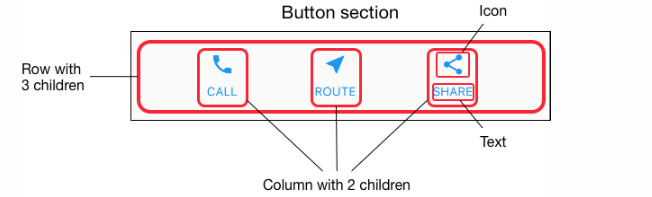
\includegraphics[width=0.8\textwidth, keepaspectratio]{Bilder/FlutterWidgetButtonSectionExample.png}
	\caption{Beispiel: Aufbau von Widgets  \cite{FlutterBuildingLayouts}}
	\label{img:FlutterWidgetButtonSectionExample}
\end{figure}

\par \medskip Ein in dem Artikel \citep[Widgets]{HackernoonFlutterArcticle} beschriebener wichtiger Aspekt ist, dass Flutter im Gegensatz zu anderen Alternativen eine eigens erstellte Systemschnittstellen-Architektur besitzt und nicht auf OEM-Widgets oder DOM-Web Views zurückgreift, wie in Abbildung \ref{img:hackernoonFlutterArcticleArchitecture} verdeutlicht wird. Dies ermöglicht eine extrem freie Handhabung und Individualisierung im Umgang mit den Widgets und Plattform spezifischen Diensten.

\bigskip
\begin{figure}[H]
	\centering
	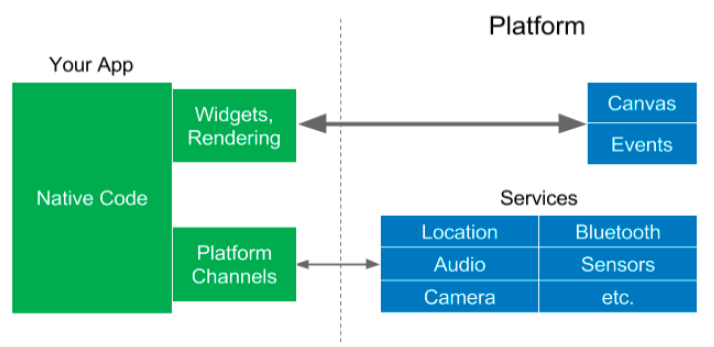
\includegraphics[width=0.8\textwidth, keepaspectratio]{Bilder/WidgetsFlutterArchitecture.png}
	\caption{Flutter Widgets Architektur \cite{HackernoonFlutterArcticle}}
	\label{img:hackernoonFlutterArcticleArchitecture}
\end{figure}

\par \medskip Diese Widgets bilden zur Laufzeit eine hierarchische Struktur und setzen sich selbst aus weiteren Widgets zusammen. Somit ist der Ursprung einer jeden Programm-Oberfläche ein Wurzel-Widget, welches wiederum Kinder-Widgets enthält und diese somit über mehrere Ebenen eine Gesamtkomposition bilden, den sogenannten \textbf{Widget Tree}. 

\par \medskip Widgets können also je nach Ausprägung beispielsweise strukturierende Elemente, wie Spalten und Zeilen sowie stil-definierende Elemente in Form von Farbdefinitionen darstellen. Weiterhin können Widgets auch Interaktion-Elemente, wie Buttons und Textfelder und noch viele weitere Elemente mit unterschiedlichen Eigenschaften definieren.

\subsection{Flutter UI Rendering}
\par Flutter verwendet im Gegensatz zu anderen Alternativen nach eigener Aussage eine selbst entwickelte und optimierte Rendering-Engine, die die Benutzeroberfläche nach einer Veränderung des aktuellen Status neu generiert und diese Veränderung dem Benutzer darstellt (vgl. \citep[What makes Flutter unique?]{Flu3}). Die folgende Abbildung \ref{img:flutterHighLevelRendering} stellt einen solchen Ablauf dar.

\bigskip
\begin{figure}[H]
	\centering
	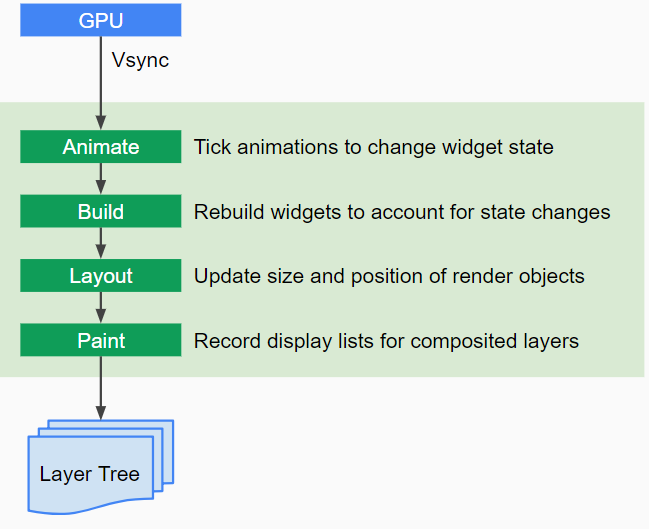
\includegraphics[width=0.8\textwidth, keepaspectratio]{Bilder/FlutterRendering.png}
	\caption{Flutter Rendering \cite{Flu5}}
	\label{img:flutterHighLevelRendering}
\end{figure}

\par Sollte sich der aktuelle Zustand der Applikation beispielsweise durch eine Benutzeraktion verändern, so werden die in der Baumstruktur vorhandenen Widgets neu generiert, deren Eigenschaften aktualisiert und dem Benutzer letztendlich angezeigt.

\newpage		
\section{Was ist Redux?}
\par Redux ist eine von Dan Abramovic und Andrew Clark entwickelte, im Jahr 2015 veröffentlichte  open-source Bibliothek für JavaScript-Anwendungen (vgl. \citep{ReduxWiki}). Durch die zentrale Verwaltung von Zustandsinformationen soll eine erleichterte Pflege der Konsistenz und aufgrund dessen auch eine \grqq einfache\grqq{} Wartbarkeit und Testbarkeit der Software ermöglicht werden. \citep[vgl. Abschnitt Read Me]{ReduxReadMe}
\par \bigskip \textit{Hinweis: Wie auch in \citep[vgl. Abschnitt Read Me]{ReduxReadMe} angemerkt wird, wird an dieser Stelle darauf hingewiesen, dass es sich hierbei nicht um das WordPress-Framework \textbf{Redux Framework}\citep{WordPressRedux} handelt.}

\par Innerhalb einer Redux-Architektur existieren verschiedene Komponenten, welche jeweils einen besonderen Zweck erfüllen und durch das modulare Zusammenspiel mit anderen Komponenten in dem System eine Gesamtkomposition bilden.
\par \bigskip Die wichtigsten Redux-spezifischen Komponenten sind \textbf{Actions}, \textbf{Reducers} und der \textbf{Store}, welche hinsichtlich Bedeutung und Funktionsweise in den nachfolgenden Kapiteln beschrieben werden:

\subsection{Actions}
\par Wie in den Basics der Online-Dokumentation \citep{ReduxActions} beschrieben wird, definieren Actions im Rahmen von Redux hauptsächlich Informationspakete, welche unter dieser Bedeutung auch als \grqq Payload\grqq{} bezeichnet werden. Sie enthalten in erster Linie nur Informationen über die Action-spezifische Operation, wie beispielsweise das Ändern bestimmter Bestandteile des aktuellen Systemzustands.
\par \bigskip \textit{Hinweis: Es könnte beispielsweise denkbar sein, dass ein neuer Eintrag einer ToDo-Liste angelegt werden soll. Hierbei würde die Action vermutlich einen Namen wie \grqq AddTodoAction\grqq{} tragen und die Informationen des Titels des neuen Eintrags enthalten. \\
Das Ausführen dieser Zustandsänderung wird also nicht von den Actions selbst ausgeführt, für diesen Zweck dienen die sogenannten Reducer-Funktionen.}

\subsection{Reducers}
\par Reducer-Funktionen erfüllen den Zweck, die durch die jeweilige Action übermittelten Informationen zu verarbeiten und die eigentliche, durch die Action spezifizierte, Zustandsänderung durchzusetzen. (vgl. \citep{ReduxReducers})
\par Reducer liegen im Allgemeinen als Pure Function (auch Reine Funktionen) vor. Dies Bedeutet im Rahmen der Redux-Architektur, dass die Funktionen keine direkten Änderungen an den durch die Actions übermittelten Informationen oder an dem Status selbst  vornehmen dürfen und unter keinen Umständen Seiteneffekte produzieren dürfen. Die Auswirkungen von Pure Functions müssen deterministisch bestimmbar sein, also muss unter den gleichen Eingabebedingungen immer das gleiche zu erwartende Ergebnis folgen.
\par Im Detail werden also nicht direkte Änderungen an Objekten vorgenommen, sondern der gesamte aktuelle Zustand durch das Neuerzeugen überschrieben.
\par \bigskip \textit{Hinweis: Eine nicht den Eigenschaften von Pure Functions entsprechenden Funktion wäre das Bestimmen des Datums mit der JavaScript-Funktion Date.now(), da hier bei Ausführung immer ein unterschiedliches Ergebnis herauskommt.}

\subsection{Store}
\par Der Store ist in der Redux-Architektur das zentrale Element, welches nicht nur für die Datenhaltung des aktuellen Zustands (State) der Applikation zuständig ist, sondern auch als Schnittstelle für die Bereitstellung und Veränderung des aktuellen Systemzustands dient (vgl. \citep{ReduxStore}).
\par Im Gegensatz zu den anderen Komponenten ist der Store innerhalb der Architektur einmalig, was viele Vorteile der Redux-Architektur überhaupt erst ermöglicht.

\par \bigskip \textit{Hinweis: Der Store enthält alle für die Applikation relevanten Informationen an zentraler Stelle im System in einem State Objekt.\\
Die gespeicherten Informationen liegen im besten Fall in normalisierter Form vor. Insgesamt ist ein flacher Key-Value Store dem Handhaben komplexer Objekte vorzuziehen}

\subsection{Flutter Redux Libary}
\par Die externe Flutter Libary \textbf{flutter\char`_redux}\citep{FlutterReduxLib} setzt die auf JavaScript basierende Redux-Funktionsweise für die Entwicklung mobiler Applikation mit Flutter und Dart um, dadurch wird die beschriebene komfortable Nutzung der Redux-Funktionsweise ermöglicht.

\par \bigskip Grundsätzlich werden also dieselben Funktionsweisen durch die Nutzung der Flutter Redux Libary abgebildet. Es folgt dennoch eine kurze Beschreibung der spezifischen Redux Widgets, welche sich jedoch alle auf die Interaktion mit dem zentralen Store beziehen:

\begin{itemize}
\item \textbf{StoreProvider}
\par Der StoreProvider ist ein Schnittstellen-Widget, das allen unterliegenden Widgets Zugang zum Store ermöglicht.
\item \textbf{StoreBuilder}
\par Der StoreBuilder holt sich den aktuellen Zustand von dem in der überliegenden Hierarchie am nächsten platzierten StoreProvider und bietet eine builder-Funktion um die fallspezifischen Informationen zu verwenden.
\item \textbf{StoreConnector}
\par Der StoreConnector trägt die Aufgabe, den von dem StoreProvider übergebenen Store durch eine converter-Funktion in ein ViewModel umzuwandeln, welches die benötigten fallspezifischen Informationen in sich hält und durch die builder-Funktion diese Informationen kontextspezifisch verwendet. Weiterhin wird der StoreConnector bei jeder Änderung des Zustands neu generiert und somit die durch das ViewModel repräsentierten Informationen aktualisiert.
\end{itemize}

\newpage
\chapter{Untersuchung des Problembereiches} \label{chap:problemanalyse}
\par Im folgenden Kapitel werden die Rahmenbedingungen und die Analysestrategie zu den durchgeführten Befragungen von Professoren und Studierenden aus dem Studiengang Informatik/Softwaretechnik der Fachhochschule Lübeck dargestellt. Die daraus resultierenden Ergebnisse und Erkenntnisse beider Seiten werden in zusammengefasster Form beschrieben. 
\par Die Diskussion dieser Ergebnisse und die, aus den durchgeführten Befragungen abgeleiteten Anforderungen an die zu entwickelnde Software, stellt das Produkt der Anforderungsanalyse und somit den Ausgangspunkt für die gesamte Arbeit dar.

\section{Hypothese}
\par Die Auseinandersetzung mit komplexen Problemstellungen, wie einer, als abschließende Prüfungsleistung des Studiums zu erarbeitende, Bachelorarbeit, stellt erfahrungsgemäß für viele Studierende eine große Herausforderung dar. Diese Herausforderung ergibt sich aus dem erstmaligen Zusammenspiel von selbstständigem und eigenverantwortlichem Arbeiten sowie dem Problemlösen mittels erworbener Fach- und Methodenkenntnisse über einen längeren Zeitraum.
Trotz des Verlaufs des Studiums, des angeeigneten Wissens und der somit zahlreich erworbenen Fähigkeiten kommt es im Kontext von Bachelorarbeiten dennoch oftmals zu Schwierigkeiten, diese Kompetenzen auf reale Probleme abzubilden und zu dokumentieren.

\newpage
\section{Identifikation der Interessengruppen}
\par Die folgende Tabelle \ref{tab:uebersichtInteressengruppen} bietet eine Übersicht der, im Rahmen des Projektes identifizierten, Interessengruppen und welche Stellung diese zu dem Projekt bezüglich Einfluss, Einstellung und Erwartungen einnehmen.

\medskip
\begin{center}
\scalebox{0.70}{
\begin{tabularx}{15cm}{X|l|l|X|X}
\toprule
\textbf{Bezeichnung} 
& \textbf{Einfluss} 
& \textbf{Einstellung} 
& \textbf{Erwartungen} 
& \textbf{Bemerkungen} 
\\ \midrule
	
\textbf{Studierende}
&  Hoch
&  Positiv
&  Erhoffen sich optimale Ergebnisse und weniger Fallstricke bei dem Bearbeiten der Bachelorarbeit und diesbezüglich eine insgesamt umfangreich ausfallende Hilfestellung.
&  Zielgruppe der zu entwickelnden Applikation.
\\ \midrule

\textbf{AStA}
&  Hoch
&  Positiv
&  Erhoffen sich eine angemessene Förderung und Entlastung der Studierenden bei der Bearbeitung der Bachelorarbeit.
&  Sprachrohr und Interessenvertreter der Studierenden.
\\ \midrule

\textbf{Leiter des Bachelorseminars}
&  Hoch
&  Positiv
&  Erhofft sich eine steigende Bereitschaft der Studierenden, im Rahmen des Bachelorseminars Beiträge zu erbringen sowie eine steigende Qualität der Vorbereitung, Bearbeitung und Fertigstellung von Bachelorarbeiten.
&  Leitet das Bachelorseminar, hat somit direkten Kontakt mit der Zielgruppe und trägt wichtige Erfahrungswerte bezüglich der Probleme der Studierenden mit sich.
\\ \midrule

\textbf{Professoren}
&   Hoch
&   Positiv
&   Erhoffen sich eine steigende Qualität der Bearbeitung der Bachelorarbeit sowie eine Entlastung bei dem Betreuen von Studierenden, hinsichtlich sich wiederholenden Erklärungen und weiterer Trivialitäten.
&  Tragen wichtige Erfahrungswerte durch den detaillierten Einblick als Betreuer von Bacheloranden sowie dem Bewerten von Bachelorarbeiten mit sich.
\\ \midrule

\textbf{Präsidium}
&  Mittel
&  Positiv
&  Erhoffen sich eine Steigerung der Leistung der Studierenden an der Fachhochschule Lübeck.
&  Machtpromotor der Fachhochschule Lübeck.
\\ \midrule
\bottomrule
\end{tabularx}}
\begin{tablenotes}
\item  
\end{tablenotes} 
\captionof{table}{Übersicht der Interessengruppen}
\label{tab:uebersichtInteressengruppen}
\end{center}

\newpage
\section{Wahl der Analysestrategie}
\par Um den Problembereich zu ermitteln und somit eine Analysegrundlage zu schaffen, werden unterschiedliche Personengruppen der Fachhochschule Lübeck durch verschiedene Befragungs- und Analysemethoden in das Projekt miteinbezogen. Dies soll einen detaillierten Einblick in die Sichtweisen der unterschiedlichen beteiligten Personen und Interessengruppen ermöglichen und somit eine Grundlage für das Verständnis der aktuellen Situation bilden.

\par Als primäre Einflussgeber, die in die Entwicklung der Applikation stark eingebunden werden, wurde die Gruppe der Professoren und die Gruppe der Studierenden identifiziert. Diese Entscheidung wurde aufgrund der im Rahmen der Bachelorarbeit existierenden unterschiedlichen Sichtweisen sowie der unmittelbaren Berührung mit dem Problembereich der Beteiligten und den unterschiedlichen Erfahrungsständen von Betreuern und Bacheloranden getätigt (siehe Abbildung \ref{tab:uebersichtInteressengruppen}). Darüber hinaus handelt es sich bei den Studierenden um die Zielgruppe und potentielle spätere Anwender, weshalb die Aufnahme der Probleme und Meinungen der Studierenden als essenziell angesehen wird. 

\bigskip
\begin{figure}[H]
	\centering
	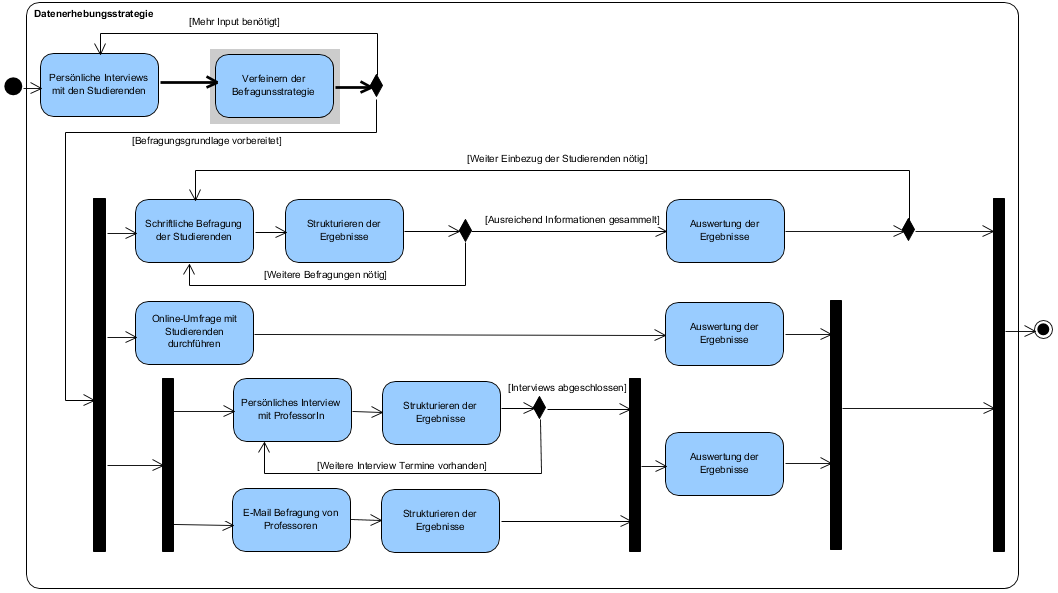
\includegraphics[width=1\textwidth, keepaspectratio]{Bilder/Diagramme/Analysestrategie.png}
	\caption{Beschreibung der Analysestrategie}
	\label{img:analysestrategie}
\end{figure}

\par Durch die initial durchgeführten Gespräche mit den Studierenden ließen sich Erkenntnisse über den Umfang des Problems gewinnen. Auf Grundlage dieser Erkenntnisse wurde die weitere Analysestrategie verfeinert und für die Umsetzung durch die Erstellung von Fragenkatalogen und Interview-Leitfaden vorbereitet (siehe Abbildung \ref{img:analysestrategie}), welche im folgenden Verlauf beschrieben werden.
\par Die Interviews mit den Studierenden sollen somit als Grundlage zu Konzeption und Design weiterer Befragungsstrategien dienen und stellen in diesem Umfang einen Ausgangspunkt für die Problemanalyse dar. Weiterhin wurden die gewählten Interviewpartner bei Zustimmung über das gesamte Projekt und nach Absprache auch in die Evaluation der Applikation miteinbezogen.

\newpage
\par Durch das Durchführen von Gruppeninterviews sollen die Studierenden zu Diskussionen angeregt werden, welche durch den Leiter des Interviews gezielt angeregt werden können. Dies hat den Zweck, die Situation und die Rolle der Studierenden für den Interviewer erkenntlich zu machen.  Diese persönlichen Interviews dienen in erster Linie also nicht der Erhebung konkreter Daten, sondern als erster Berührungspunkt mit dem Problembereich und in diesem Rahmen als strategischer Orientierungspunkt für das weitere Vorgehen.

\subsection{Einbezug der Professoren}
\par Für die Interessengruppe der Professoren aus dem Fachbereich Informatik wurden als Grundlage der Datenerhebung Einzelinterviews mit einer ausgewählten Gruppe von Professoren durchgeführt, während eine weitere Gruppe von Professoren schriftlich per E-Mail befragt wurde (siehe Abbildung \ref{img:analysestrategie}). Dies bietet sowohl den Zugriff auf die unmittelbaren Erfahrungen der einzelnen Professoren als Spezialisten in ihren jeweiligen Fachgebieten, als auch auf die Erfahrungen der Professoren in der Position eines Betreuers und Ansprechpartners für Bacheloranden. 
\par \bigskip Durch das Durchführen von Einzelinterviews wird ermöglicht, die Erwartungen seitens der Professoren an die Bacheloranden im Detail zu identifizieren und die in dieser Hinsicht priorisierten inhaltlichen und methodischen Aspekte bei der Bearbeitung einer Bachelorarbeit herauszuarbeiten. Die Aufteilung auf Einzelinterviews und E-Mail Befragungen bietet den Vorteil, beide Strategien simultan zu verfolgen und nach Abschluss der Datenerhebung sowohl die detaillierten Einzelinterviews, als auch die oberflächlicher ausfallenden E-Mail Antworten in bereits dokumentierter Form vorliegen zu haben, um diese dann auszuwerten.

\subsection{Einbezug der Studierenden}
\par Nach Absprache mit den interviewten Studierenden werden diese weiterhin per schriftlicher Befragung in die Entwicklung des Projektes, unter ergänzender Zunahme anderer Studierender, eingebunden.In diesem Zusammenhang werden die teilnehmenden Studierenden mittels Bildern, Fragen und Gestaltungsideen der Applikation regelmäßig über den aktuellen Stand der Entwicklung informiert. Auf diese Weise sollte es möglich sein, ein breites, jedoch persönliches Feedback zu erhalten, da sich die Einbindung der Studierenden auf diese Weise sehr gut automatisieren lässt. Wesentlich dabei ist auch die Tatsache, dass die Reaktionsfreudigkeit der Studierenden höher ausfällt, als für die im Vergleich existierende Alternative der zeitaufwändigeren persönlichen Interviews.
\par \bigskip Aufgrund der Durchführung der schriftlichen Befragung wird der Ablauf bereits dokumentiert und der Fragesteller sowie die Studierenden haben jederzeit die Möglichkeit Fragen und Anregungen zu teilen. Miteinbezogen werden vorzugsweise Studierende der oberen Semester, unabhängig davon, ob sie sich vor Beginn, während der Bearbeitung oder nach Abschluss der Bachelorarbeit befinden, da die unterschiedlichen Sichtweisen und Erfahrungsstände wichtige Impulse für die Entwicklung der Applikation geben.

\newpage
\section{Ergebnisse der Professoren}
\par Im Folgenden sind die gewonnenen Eindrücke und Kenntnisse der Einzelinterviews mit den Professoren des Fachbereichs Informatik durch Themenkategorien geordnet und in zusammengefasster Form dokumentiert.
\par Es haben insgesamt sechs Professoren an persönlichen Einzelinterviews teilgenommen, wobei es für fünf Interviews gestattet wurde, eine Tonaufzeichnung anzufertigen.
\par\medskip Des Weiteren wird auch eine schriftliche Befragung miteinbezogen, die jedoch das gleiche Fragespektrum wie die Interviews einnimmt.
\par\bigskip \textbf{Allgemeine Informationen}
\par Der zeitliche Rahmen der fünf aufgezeichneten Interviews erstreckt sich über einen Zeitraum von etwa 30 bis 45 Minuten. Für die Auswertung der aufgezeichneten Interviews wurden die Aussagen der Interviewpartner, auf Grundlage der vorliegenden Audioaufnahmen, unter Berücksichtigung des Kontextes aufbereitet und werden nachfolgend dargestellt. Ein weiteres Einzelinterview, dass nicht aufgezeichnet wurde, erstreckte sich über einen Zeitraum von 75 Minuten. Für dieses Interview wurden lediglich begleitende Feldnotizen angefertigt. Diese Feldnotizen wurden im Anschluss des Interviews aufbereitet und fließen zusammen mit den Ergebnissen der schriftlichen Befragung in die folgende Beschreibung ein.
\par\medskip Die gewählten Kategorien ergeben sich aus dem gewählten Auswertungsverfahren, was sich an der qualitativen Inhaltsanalyse nach Mayring\citep{Mayring2015} orientiert und basieren in diesem Kontext auf die, gemäß des Verfahrens, herausgearbeiteten Codings.

\par \bigskip Die Interviews mit den einzelnen Professoren sind in transkribierter Form im Anhang zu finden (siehe Anhang \ref{anhang:interviewProfessorenTranskripte}).

\newpage
\subsection{Art der Arbeit}
\par Im Laufe der Interviews wurden verschiedene Typen von Bachelorarbeiten versucht zu identifizieren. Dabei geht es vor allem darum, die Vielfalt der typischen Arbeiten des Studiengangs Informatik/Softwareentwicklung zu erfassen und somit einen Überblick über die Situation zu bekommen.
\par \medskip Als allgemeinen auftretende Arten von Bachelorarbeiten wurden die Klassen \textit{Entwickelnde Arbeit}  und \textit{Evaluierende Arbeit} identifiziert. Weiterhin gibt es auch \textit{Reine Literaturarbeiten}, welche in dem Studiengang Informatik/Softwareentwicklung jedoch nicht oder nur in einem sehr geringen Vorkommen auftreten.

\par\medskip Es folgt eine stichpunktartige Aufführung der gewonnenen Erkenntnisse:


\par \bigskip \textbf{Konstruktiv/Entwickelnd - Durchlauf des Softwareentwicklungszyklus}
\par \medskip Die Art der konstruktiven/entwickelnden Arbeiten, befassen sich hauptsächlich mit dem Durchlaufen des Softwareentwicklungszyklus. Im Rahmen der Bachelorarbeit werden die verschiedenen Aufgaben der Softwareentwicklung, je nach Schwerpunkt der Arbeit, mehr oder weniger intensiv von dem Bacheloranden bearbeitet und beschrieben.
\par \medskip Typischer fachlicher Inhalt einer solchen Arbeit könnte sein:
\begin{itemize}
\item[\textbf{1.}] Anforderungsanalyse
\item[\textbf{2.}] Entwurf einer Softwarearchitektur
\item[\textbf{3.}] Implementierung eines Softwareprototyps
\item[\textbf{4.}] Evaluation des Softwareprototyps
\end{itemize}

\par \medskip Typische Aufgabenstellungen:
\begin{itemize}
\item Entwicklung einer mobilen Applikation zur Interpretation von Bildmaterial.
\item Entwicklung einer mobilen Applikation zur Steigerung der Bereitschaft bei Senioren und Seniorinnen Fitnessaktivitäten auszuführen, unter Einbezug von  Gamification-Elementen.
\item Entwicklung einer Software zur Optimierung der täglichen Arbeitsabläufe im Unternehmen A.
\end{itemize}

\par \medskip Ein bei externen Arbeiten wichtiger Aspekt sind die möglichen Interessenunterschiede zwischen dem externen Unternehmen und dem internen Betreuer der Fachhochschule, welche einen Einfluss auf die Inhalte der Bachelorarbeit haben können. Externe Unternehmen sind tendenziell eher an dem resultierenden Ergebnis interessiert, während die internen Betreuer darüber hinaus einen hohen Wert auf nachvollziehbare Methodik, Herangehensweise sowie Planung und das saubere wissenschaftliche Arbeiten legen und somit ein  hohes Interesse an dem Gesamtprozess haben.

\newpage
\par \bigskip \textbf{Analytisch/Evaluierend - Vergleich, Auswertung und/oder Nachweis eines Aufgabengegenstandes}
\par \medskip Die Art der analytisch/evaluierenden Arbeiten beinhalten hauptsächlich die Analyse und Auswertung eines Aufgabengegenstandes oder mehrerer verschiedener Aufgabengegenstände. Es wird der gesamte Weg der Analysestrategie, der Durchführung der Analyse und der Auswertung behandelt.
\par \medskip Typischer fachlicher Inhalt einer solchen Arbeit könnte sein:
\begin{itemize}
\item[\textbf{1.}] Erstellen eines Kriterienkatalogs
\item[\textbf{2.}] Aufbau des Experiments
\item[\textbf{3.}] Durchführung des Experiments
\item[\textbf{4.}] Evaluation und Ergebnisauswertung
\end{itemize}

\par \medskip Typische Aufgabenstellungen könnten sein:
\begin{itemize}
\item Evaluation der Gesichtserkennungsdienste von Unternehmen A, Unternehmen B und Unternehmen C.
\item Untersuchung des Verhaltens einer neuen Technologie A, im Vergleich mit einer alten Technologie B.
\item Datenbankanalyse unter Anwendung von Machine-Learning-Algorithmen.
\end{itemize}

\par \bigskip \textbf{Reine Literaturarbeiten}
\par Reine recherchierende Arbeiten finden in dem Studiengang Informatik/Softwareentwicklung aufgrund dem geringen Interesse seitens der Studierenden kaum statt und werden aus Gründen der Vollständigkeit lediglich erwähnt und nicht ausgeführt.

\newpage
\subsection{Erwartungen an den Bacheloranden}
\par Im Laufe der Interviews wurden die Professoren hinsichtlich Ihrer Erwartungen an die Bacheloranden befragt und haben in diesem Rahmen häufig gleiche oder ähnliche Punkte ausgeführt. Aus diesem Grund werden im folgenden Verlauf die Meinungen der befragten Professoren aus der Sicht als Betreuer zu den jeweiligen Aspekten als zusammengefasstes Meinungsbild wiedergegeben.

\par\medskip Es folgt die Ausführung der gewonnenen Erkenntnisse:

\par \bigskip \textbf{Selbständiges Arbeiten}
\par Das selbstständige Arbeiten und Vorgehen ist eine der am häufigsten genannten Erwartungen, was sich in unterschiedlichen Punkten äußert. Dazu zählen vor allem das selbständige Kommunizieren von Ergebnissen und das Einholen von Feedback sowie die Transparenz bei Problemen oder Schwierigkeiten, um sich Hilfe von dem Betreuer zu holen. Es wurde mehrfach betont, dass es im Allgemeinen nicht die Aufgabe des Betreuers ist, nachzufragen und aufzufordern. Das Einbinden des Studierenden in die Erarbeitung der Aufgabenstellung ist ein häufig genannter Punkt, der bereits frühzeitig Engagement des Studierenden erfordert.
\par Des Weiteren stellt das selbstständige Einarbeiten in die Probleme und die Auswahl geeigneter Methoden und Werkzeuge einen wesentlichen Inhalt der Arbeit dar.
\par \bigskip \textbf{Die Vorgehensweise}
\par Sehr häufig wird betont, dass die Vorgehensweise hinsichtlich der wissenschaftlichen Arbeitsweise von essenzieller Bedeutung ist. In diesem Rahmen soll der Studierende auch zeigen, dass er in der Lage ist, große Probleme systematisch in Teilprobleme zu zerlegen und diese unter Berücksichtigung der im Studium vermittelten Methoden, Modelle und Techniken zu bearbeiten. Sehr wichtig ist dabei das vorausschauende Planen von Teilprozessen, wie beispielsweise das Evaluieren der Ergebnisse. Dies sollte von Anfang an berücksichtigt werden und die in diesem Rahmen getroffenen Entscheidungen sollten nachvollziehbar erklärt werden können. Dazu zählt weiterhin das Erstellen eines Zeitplans, welcher sich im Verlauf jedoch durchaus verändern kann. Es wird sehr viel Wert darauf gelegt, zu sehen, dass die Studierenden einen weiten Blick auf das gesamte Projekt entwickeln und pflegen.
\par \bigskip \textbf{Der Literaturteil}
\par Es wird betont, dass vor allem Wert auf einschlägige Quellen gelegt wird. In diesem Zusammenhang ist es wichtig, dass die Studierenden Literaturquellen verwenden sollten, die bereits eine anerkannte längere Gültigkeit besitzen. Weiterhin sollten die Studierenden über den Umfang von Grundlagenliteratur hinaus blicken und je nach Themengebiet und Arbeitsstand spezifischere Fachliteratur in die Arbeit einbeziehen. Dies kann auch bedeuten, dass auf wissenschaftliche Papiere und Primärquellen verwiesen werden soll. Je nach Thema und Aufgabenstellung kann der Literaturteil mehr oder weniger umfangreich ausfallen, was sich durch dem praktischen Teil der Arbeit ausgleichen lässt.

\newpage
\par \bigskip \textbf{Der praktische Teil}
\par Im Wesentlichen soll der praktische Teil den Umfang der Aufgabenstellung abdecken und gegebene und/oder erhobene Anforderungen erfüllen. Je nach Thema und Aufgabenstellung der Arbeit nimmt dieser Teil einen höher oder niedriger ausfallenden Umfang ein.
Der Studierende soll bei der praktischen Bearbeitung der Aufgabe zeigen, dass er in der Lage ist, im Studium gelerntes Wissen sowie kennengelernte Methoden und deren Ausführung umzusetzen. 
\par \bigskip \textbf{Das Ergebnis der Bachelorarbeit}
\par Grundsätzlich soll die Bachelorarbeit aus zwei Teilen von Leistungen bestehen. Die von dem Studenten durchgeführte Literaturarbeit nimmt einen Teil der Arbeit ein, während die eigenständige praktische Leistung den anderen Teil erfüllt. Der Umfang der jeweiligen Anteile kann dabei je nach Themengebiet und Aufgabenstellung stark variieren.
\par Das angestrebte Ziel der Aufgabenstellung einer Bachelorarbeit, welches sich je nach Art der Arbeit stark voneinander unterscheiden kann, soll wissenschaftlich erarbeitet und somit nachvollziehbar und belegbar sein und im Optimalfall die Aufgabenstellung erfüllen. Es kann jedoch auch vorkommen, dass das angestrebte Ziel aus verschiedenen Gründen nicht erreicht wurde. Dies muss nicht bedeuten, dass es zu einer schlechten Bewertung der Bachelorarbeit kommt, sofern der Grund oder die Erkenntnis über ein bestimmtes aufgetretenes Problem belegbar und nachvollziehbar dokumentiert ist.

\newpage
\subsection{Häufig auftretende Probleme}
\par Es stellte sich im Verlauf des Interviews heraus, dass Studierende immer wieder mit gleichen oder ähnlichen Problemen zu kämpfen haben. Im folgenden Verlauf werden diese genannten Probleme in aufbereiteter Form stichpunktartig beschrieben.

\par \medskip Es folgt die Ausführung der gewonnenen Erkenntnisse:

\par \bigskip \textbf{Zeitmanagement}
\par Der am häufigsten genannte Aspekt ist das mangelhafte Zeitmanagement der Studierenden. Im Laufe der Bearbeitung der Bachelorarbeit kommt es häufig zur Unterschätzung des nötigen  Zeitaufwandes, besonders hinsichtlich des Schreibens der Dokumentation. 
\par Viele Studierende verschieben das Schreiben der Dokumentation auf einen späteren Zeitpunkt und geraten im späteren Verlauf der Bearbeitungszeit somit unter Zeitdruck. Die Betreuer haben unter diesen Umständen wenige Möglichkeiten rechtzeitiges und hilfreiches Feedback zu liefern. Es wird häufig empfohlen frühzeitig mit dem Schreiben zu beginnen und begleitend zum Arbeitsfortschritt die Dokumentation an mehreren Stellen wachsen zu lassen. Trotz vieler Hinweise seitens der Betreuer kommt es in diesen Belangen häufig zu großen Problemen.
Das Problem des mangelnden Zeitmanagements äußert sich auch darin, dass die Studierenden sich bei der Bearbeitung in nicht relevanten Details verlieren, da sie die Schwerpunkte der Arbeit nicht erkennen.
\par \bigskip \textbf{Wissenschaftliches Arbeiten}
\par Die Studierenden erfassen teilweise nicht die Bedeutung des wissenschaftlichen Arbeitens. Es kommt immer wieder zu Schwierigkeiten und Unklarheiten über den eigentlichen Umfang der Arbeit und wodurch sich das wissenschaftliche Arbeiten auszeichnet. Oft wird der falsche Umgang mit Literatur und Quellen als negatives Beispiel genannt.
\par Ein Kritikpunkt ist, dass es in dem Studiengang Informatik/Softwareentwicklung keinen Kurs gibt, welcher die Studierenden auf das wissenschaftliche Arbeiten vorbereitet. In einigen Wahlpflichtmodulen werden diesbezüglich zwar Ansätze im Rahmen von Projekten integriert, jedoch gilt dies somit nur für die an dem Wahlpflichtmodul teilnehmenden Studierenden und steht auch nicht im Fokus der Projektarbeit.
\par \bigskip \textbf{Kommunikation}
\par Kommunikation und Transparenz ist ein weiteres angesprochenes Problem. Es kommt vor, dass Studierende und Betreuer unterschiedliche Ansichten über die Zusammenarbeit haben, die sich dadurch äußern, dass die Studierenden auf Aufforderungen bezüglich Leistungsständen oder Ergebnissen seitens der Betreuer warten oder sich sogar aus diversen Gründen nicht trauen, ihren aktuellen Arbeitsstand oder ihre Probleme mit dem Betreuer zu teilen. 
\newpage
\par \bigskip \textbf{Die Vorbereitung der Studierenden}
\par Bei der Vorbereitung der Studierenden nennen die beteiligten Interviewpartner unterschiedliche Aspekte, es wird zum einen das mangelhafte selbständige Informieren der Studierenden kritisiert, andererseits wird jedoch auch eine optimaler zu gestaltende Vorbereitung der Studierenden seitens der Fachhochschule für den Studiengang Informatik/Softwareentwicklung betont.
\par \medskip Das angebotene Bachelorarbeit-Seminar wird positiv erwähnt, da es einen positiven Einfluss auf die Arbeit der Studienenden hat. Es müssen weniger Aspekte einer Bachelorarbeit erklärt werden, jedoch müssen viele Aspekte mehrfach wiederholt werden. 
\par Es wird betont, dass auch viele Informationsmaterialien im Lernraum der Fachhochschule Lübeck zu finden seien, auf die auch oft hingewiesen wird, jedoch von den Studierenden nicht in dem Umfang beachtet werden, für den die Materialien gedacht sind. Dabei wird unter anderem auch kritisiert, dass die Informationsmaterialien teilweise schwer auffindbar sind, da sie nicht an einer zentralen Stelle, sondern verteilt im Lernraum liegen. 
\par Weiterhin wird jedoch auch betont, dass die Studierenden zu wenig Engagement aufbringen, sich trotz vieler Möglichkeiten selbstständig zu informieren. 

\subsection{Die Applikation – Wünsche und Anregungen}
\par In den Interviews wurden die Professoren nach ihren persönlichen Wünschen, Ideen und Anmerkungen bezüglich der Applikation gefragt. Es folgt die Ausführung der aufgenommenen Wünsche und Ideen.

\par \bigskip \textbf{Neuer Kanal zu den Studierenden}
\par Es wird der Wunsch geäußert, dass die Applikation verwendet werden kann, um in zentraler Form konkrete interne oder externe Bachelorarbeit-Themen sowie Beispielthemen angeben zu können, da dies an der Fachhochschule Lübeck bisher nicht ermöglicht ist.
\par \bigskip \textbf{Plattform als Informationsquelle}
\par Es besteht der Wunsch, die im Lernraum vorliegenden Informationsmaterialien, durchaus auch in aufbereiteter Form, durch die Applikation den Studienreden zugänglicher zu machen.
\par \bigskip \textbf{Applikation zur Unterstützung des Zeitmanagements}
\par Es wird der Wunsch geäußert die Studierenden bei dem Zeitmanagement, unter anderem durch Erinnerungen, zu unterstützen. In diesem Rahmen wird der Vorschlag eingebracht möglichst detaillierte Beschreibungen von Arbeitspaketen in dem Tool zu verlangen, damit die Studierenden dazu gezwungen sind, sich rechtzeitig mit der Aufwandseinschätzung zu beschäftigen.


\newpage
\subsection{Die Applikation - Chancen und Risiken}
\par In jedem Interview bekamen die Professoren abschließend die Möglichkeit, ihre Erwartungen an eine solche Applikation auszuführen und besonders auf die, aus ihrer Sicht, möglichen Chancen und Risiken einzugehen. 
\par \bigskip Diese Anmerkungen werden im folgenden Verlauf zusammengefasst dargestellt:
\par \bigskip \textbf{Chancen}
\begin{itemize}
\item Die Applikation als neuer Kanal für die Studierenden, der dafür dienen kann, dass Studierende sich besser informieren können. Dies wird besonders in Bezug auf die Formalien einer Bachelorarbeit betont, da viele Studierende gar nicht wissen, was die Rahmenbedingungen einer Bachelorarbeit sind oder welche Regeln und Anforderungen es überhaupt gibt.
\item Die Applikation kann im Gegensatz zum Bachelorseminar begleitend während der eigenen Bachelorarbeit genutzt werden kann. Dies kann dafür sorgen, dass die Aufnahmebereitschaft der Studierenden für Tipps, Empfehlungen und weiteren Aspekten gesteigert wird, da sie sich zu diesem Zeitpunkt mit dem Problem konfrontiert sehen und somit der Lerneffekt am höchsten ist. In diesem Ansatz wird auch die Chance erkannt, dass der Fokus der Studierenden zum richtigen Zeitpunkt auf bestimmte wichtige Fragen gelenkt werden kann und somit grobe Fehler minimiert werden können.
\item Besseres Zeitmanagement der Studierenden und die somit geförderten organisatorischen Fähigkeiten der Studenten.
\item Die App könnte Probleme im Projektmanagement und bei der Gestaltung der Dokumentation minimieren.
\item Das Senken des Beratungsaufwandes für Professoren und somit das Minimieren von sich wiederholenden Arbeitsabläufen für die unterschiedlichen Bacheloranden wird als Chance genannt, da in einfacher Form auf eine Applikation verwiesen werden kann, die alle nötigen Informationen enthält.
\end{itemize}

\newpage
\par \bigskip \textbf{Risiken}
\begin{itemize}
\item Die Applikation kennt nicht den realen Stand der Bachelorarbeit, sondern die Studierenden sind für die Verwaltung selbst zuständig. Wenn der Benutzer eine der Aufgaben abhakt, stellt dies unter Umständen nicht den echten Zustand der Bachelorarbeit dar und könnte dem Studierenden einen falschen Eindruck des Fortschritts geben.
\item Die Applikation regt dazu an, sich durch das Zeitmanagementtool zu über-planen, was dafür sorgt, dass der Benutzer von der eigentlichen Arbeit abgehalten wird. In diesem Rahmen kann die Applikation dem Benutzer nicht die Eigenverantwortung abnehmen. Der Studierende kann der Applikation nicht die Schuld für einen Misserfolg geben.
\item Gamification-Elemente könnten unter Umständen einen sehr begrenzten Effekt haben, da sie kein Interesse an einem Thema wecken können, sondern das Grundinteresse aus der Eigenmotivation erzeugt werden muss.
\item Befürchtung, dass Studenten gegebenenfalls die Applikation als Leitfaden als unumstößlich ansehen könnten und somit durch unterschiedliche Ansichten in einen Konflikt mit dem Betreuer geraten können.
\item Die App könnte missverstanden werden als Ersatz für die persönliche Betreuung – insbesondere fachliche Aspekte wird eine App naturgemäß nicht abdecken können. Es könnte weiterhin zu einem \grqq Device Mismatch\grqq{} kommen, da Bachelorarbeiten üblicherweise nicht an mobilen Endgeräten entstehen man müsste also immer zwei Geräte bedienen: Notebook/Desktop-PC und Smartphone.
\item Die Applikation könnte den Studierenden zu sehr unterstützen, sodass die eigentliche Arbeit der Prüfungsleistung gar nicht von den Studierenden selbst ausgeführt wird, sondern durch die Applikation. Dies könnte zu einer Minderung des Lerneffektes bei der Bearbeitung der Bachelorarbeit führen.

\end{itemize}

\newpage
\section{Ergebnisse der Studierenden}
\par Das folgende Kapitel liefert einen Einblick in die Ergebnisse der Befragung der Studierenden und beschreibt die in diesem Rahmen gewonnenen Erkenntnisse.
\par Im Fokus der Befragung stehen die Erwartungen an die Bachelorarbeit und den Betreuer und die typischen Probleme und Sorgen der Studierenden. Die Erkenntnisse der Befragung werden abschnittsweise in zusammengefasster Form dargestellt. Die gesamten Antworten der schriftlich befragten Studierenden ist in kategorisierter Form im Anhang zu finden (siehe \ref{anhang:schriftlicheBefragungStudierendeZusammenfassung}). Weiterhin stehen auch die nicht aufbereiteten Originalaufzeichnungen der schriftlichen Befragung zur Verfügung, allerdings aufgrund des Umfangs nur in elektronischer Form auf der CD im Anhang (siehe TODO).

\label{sub:studentenchriftlichErgebnisse}
\par \bigskip Informationen zu der schriftlichen Befragung:
\begin{itemize}
\item Insgesamt wurden 17 Studenten schriftlich befragt.
\end{itemize}

\subsection{Erwartungen an den Betreuer}
\par In diesem Kapitel werden die ermittelten Erwartungen der Studierenden an den Betreuer einer Bachelorarbeit zusammengefasst beschrieben. 

\par \bigskip \textbf{Teilen von Erfahrungen}
\par Es werden sich Erkenntnisgewinne durch das Teilen von Erfahrungen der Betreuer gewünscht, was sich besonders auf die Arbeit mit externen Unternehmen bezieht. Hierzu zählen Hinweise zu Besonderheiten und die wichtigen Unterschiede zu einer internen Bachelorarbeit. 
\par Weiterhin wird das gemeinsame Erarbeiten eines Themas, was bezüglich des Umfangs durch die Erfahrungen des Betreuers eine angemessene Form annehmen sollte, betont.

\par \bigskip \textbf{Kommunikation}
\par Was die Kommunikationsbereitschaft betrifft, wird vor allem eine hohe Erreichbarkeit, das (schnelle) Beantworten von Fragen und die Möglichkeit, persönliche Treffen wahrnehmen zu können, von dem Betreuer erwartet.

\par \bigskip \textbf{Feedback}
\par Grundsätzlich wird von dem Betreuer erwartet, dass dieser sich mit der Bachelorarbeit der Studierenden insofern beschäftigt, als dass die einzelnen Feedback-Punkte zum aktuellen Stand, Inhalt, Ideen und Umfang konstruktiv diskutiert werden können. Darüber hinaus erwarten die Studierenden, dass der Betreuer Hinweise bei Unverständlichkeiten der Dokumentation gibt und gegebenenfalls schlechte Ideen und Entwurfsentscheidungen hinterfragt.
\par In diesem Rahmen wird auch vereinzelt erwartet, dass der Betreuer Interesse an der Arbeit des Studierenden hat sowie Bereitschaft für die Beantwortung von Fragen und auf das Diskutieren von Lösungsmöglichkeiten eingeht.

\par \medskip \textbf{Impulse des Betreuers}
\par In wenigen Fällen erwarten die befragten Studierenden, dass der Betreuer aktiv an dem Prozess der Erstellung der Bachelorarbeit teilnimmt. Das bezieht sich auf die Unterstützung bei Zeitmanagement, dem Geben von Denkanstößen und Anregungen und das vom Betreuer ausgehende Einfordern von Leistungen.

\subsection{Die größten Probleme der Studierenden}
\par Die Studierenden wurden zu ihren, nach eigener Einschätzung, größten Unsicherheiten und Problemen gefragt und haben einige, sich im Laufe der Befragung wiederholende, Aspekte angesprochen, die im folgenden Verlauf zusammengefasst werden.

\par \bigskip \textbf{Schreiben der Dokumentation}
\par Die von den Studierenden angesprochenen Punkte befassen sich in erster Linie mit Unsicherheiten bei der Einschätzung von Umfang, Inhalt und Aufbau der Dokumentation. 
\par Des Weiteren werden Rechtschreibung und der korrekte Umgang mit Quellen genannt.

\par \bigskip \textbf{Zeitmanagement}
\par Der Punkt Zeitmanagement stellt für viele Studierende eine grundsätzliche Herausforderung dar.

\par \bigskip \textbf{Fachliche Probleme}
\par Teilweise werden auch fachliche Probleme unterschiedlicher Natur als große Herausforderung genannt. Dazu zählen zum einen Probleme mit der im Rahmen der Bachelorarbeit zu verwendenden Hardware, andererseits aber auch Softwareprobleme, das Entwickeln von sinnvollen Tests und das präzise Ermitteln von Anforderungen.

\par \bigskip \textbf{Sonstige Probleme}
\par Weitere Probleme, die vereinzelt genannt werden, sind Probleme mit der Themenfindung, die Kommunikation zwischen internem Betreuer und der externen Firma oder die allgemeine Überforderung bei der Bearbeitung der Bachelorarbeit.

\newpage
\subsection{Wunsch nach besserer Vorbereitung auf die Bachelorarbeit}
\par Um das Bild der Situation der Studierenden besser zu verstehen und darüber hinaus auch Impulse für die Applikation zu erfassen, wurden die Studierenden hinsichtlich Verbesserungsvorschlägen für den Verlauf des Studiums, unter dem Aspekt, was ihnen zu einer besseren Vorbereitung zur Bearbeitung der Bachelorarbeit verhelfen würde oder verholfen hätte, befragt.

\par \bigskip \textbf{Zeitmanagement}
\par Im Allgemeinen wünscht sich ein großer Teil der Studierenden eine bessere Vorbereitung bezüglich des Zeitmanagements. Die Studierenden bemängeln eine unzureichende Vorbereitung auf das Abschätzen von Zeitaufwand sowie Planung von größeren Projekten und nennen in diesem Zusammenhang den Wunsch nach Möglichkeiten und Maßnahmen im Studium, wie das häufigere Einbinden von Projektarbeiten.

\par \bigskip \textbf{Wissenschaftliches Arbeiten}
\par Häufig wird der Wunsch nach besserer Vorbereitung auf das wissenschaftliche Arbeiten genannt, es gibt Unsicherheiten bezüglich des Aufbaus einer wissenschaftlichen Arbeit, des Umgangs mit Quellen und des korrekten Einbindens von Quellcode-Inhalten. Als vorkommender Lösungsvorschlag wird ein Kurs, welcher zur besseren Vorbereitung vor dem 6. Semester stattfinden sollte, genannt.

\par \bigskip \textbf{Aufklärung zur Bachelorarbeit}
\par Viele der befragten Studierenden wünschen sich vorbereitende und informierende Maßnahmen zur Bachelorarbeit. Dies bezieht sich vor allem auf das Klären organisatorischer Fragen, der wichtigen Formalien und des Umfangs der Bachelorarbeit. Im Detail werden auch vorbereitende Maßnahmen gewünscht, die sich auf die Vor- und Nachteile einer extern oder intern betreuten Bachelorarbeit beziehen.

\par \bigskip \textbf{Sonstige Anmerkungen}
\par Weiterhin treten bei der Befragung auch Fälle auf, bei denen keine expliziten Veränderungen gewünscht werden, da die Studierenden zufrieden sind. Der Wunsch nach einem stärkeren Fokus auf Design-Pattern im Laufe des Studiums wurde einmal geäußert.


\newpage
\subsection{Einbezug der Studierenden in die Gestaltung der Applikation}
\par\medskip Die Einbindung der Studierenden befasst sich mit spezifischeren Fragen, hinsichtlich der motivierenden Gamification-Inhalte der zu entwickelnden Applikation. Der Verlauf der folgenden Befragungen fand somit nicht in einem Durchlauf statt, sondern ergab sich aus dem kontinuierlichen Einbinden der Studierenden. Es wurden bei der Befragung zwei Gamification-Ansätze vorgestellt.
\par\medskip Der erste Ansatz fällt unter anderem in die Benutzergruppe der \textbf{Socialiser} (Siehe Kapitel \ref{sec:grundlagenkapitelGamification}). Inhalt des Ansatzes ist es, die Motivation durch den sozialen Kontakt und Austausch mit anderen Teilnehmern zu erzeugen, indem diese den Fortschritt bei der Bearbeitung der Bachelorarbeit anderer Studierender sehen können.
\par\medskip Als Gegengewicht zum ersten Ansatz orientiert sich der zweite Ansatz an der Benutzergruppe \textbf{Achievers} (Siehe Kapitel \ref{sec:grundlagenkapitelGamification}). Dieser Ansatz beruht vor allem auf dem Abschließen und Sammeln von Erfolgen. Im Rahmen der Applikation wird es dem Benutzer bei dieser Idee ermöglicht, Erfolge durch Erfüllen von definierten Aufgaben zu erlangen und somit den Fortschritt des Projektes durch das Abschließen von geeigneten Aufgaben zu verfolgen.

\par\medskip Primäres Ziel des Einbezugs der Studierenden ist, zu bestimmen, welche Einbindung von Gamification-Strategien ansprechend auf die Zielgruppe der Studierenden wirken und in welcher Weise sich das Einbinden von Gamification-Elementen auf die Steigerung der Motivation von Studenten bei der Bearbeitung der Bachelorarbeit auswirkt.

\par\medskip In der folgenden Tabelle werden die Ergebnisse der Befragung verdeutlicht:\\\\

\begin{tabularx}{\textwidth}{l|X|c}
	\hline
	\multirow{2}*{\textbf{Art der Gamification-Strategie}} & \textbf{Art der Reaktion} & 
	\textbf{Häufigkeit} \\ \hline
	\multirow{3}*{Motivation durch soziale Interaktion} & Positiv & 3 \\
	& Negativ & 12 \\
	& Neutral & 2 \\ \hline
	\multirow{3}*{Sammeln von Achievements und Erfüllen von Aufgaben} & Positiv & 15 \\
	& Negativ & 1 \\
	& Neutral & 1 \\ \hline
	&  & \textbf{17} \\
\end{tabularx}
\captionof{table}{Einbezug der Studierende in Wahl der Gamification-Strategie}
\label{tab:einbezugStudierende}

\newpage
\section{Untersuchung der Ergebnisse}
\par Im folgenden Kapitel werden alle relevanten Kenntnisse, die aus der Datenerhebung und -auswertung hervorgehen, untersucht und analysiert. Dazu gehört die Identifikation des Problembereiches, die Auswahl der zu verfolgenden Motivationsstrategie bezüglich der Wahl der Spiel-Design-Elemente sowie die relevanten Produktfunktionen und deren abgeleitete Anforderungen, Chancen und Risiken.

\subsection{Identifikation des Problembereichs}
\par Durch die Befragung der Beteiligten und der Analyse der gewonnen Informationen haben sich die Erwartungen der Beteiligten an die Benutzung der Applikation herausarbeiten lassen, welche in der folgenden Tabelle (siehe Listing \ref{tab:erwartungenBeteiligte}) dargestellt sind.
\par Die dabei genannten Ziele und Erwartungen entsprechen dem allgemeinen Bild, das durch die Interviews und schriftlichen Befragungen ermittelt werden konnte, weshalb kleine Abweichungen in dieser Tabelle nicht mit aufgenommen wurden, da diese einen zu großen verzerrenden Einfluss auf das Gesamtbild hätten.\bigskip

\begin{tabularx}{\textwidth}{l|X}
	\toprule
	\textbf{Bezeichnung der Beteiligten} & \textbf{Wünsche der Beteiligten} \\ \midrule
	{\textbf{Professoren}}
	& Steigerung der Fragebereitschaft von Studierenden\\
	& Weniger Aufwand in das sich wiederholende Informieren des Studierenden stecken\\ 
	& Zielgerichtetere Vorbereitung auf Besprechung mit dem Betreuer\\
	& Höhere Qualität von Abschlussarbeiten und Dokumentationen\\
	& Bessere Zeitplanung der Studierenden\\
	& Systematische(re) Vorgehensweise der Studierenden\\
	\multirow{6}*{\textbf{Studierende}} & Optimale Vorbereitung auf die Bearbeitung der Bachelorarbeit\\ \midrule
	& Optimales Ergebnis der Bachelorarbeit\\
	& Kenntnisse über Formalien, Umfang und Ablauf der Bachelorarbeit\\
	& Kontrolle über die Bachelorarbeit und den Ablauf\\
	& Unterstützung \\
	& Weniger Fallstricke bei der Bearbeitung der Bachelorarbeit\\ \bottomrule
\end{tabularx}
\captionof{table}{Erwartung der Beteiligten an die Applikation}
\label{tab:erwartungenBeteiligte}

\par \bigskip Aus den Ergebnissen der Befragungen geht hervor, dass die Probleme nicht in den unterschiedlichen Ansichten der Studierenden und der Professoren liegen, da beide beteiligte Gruppen sehr kompatible Erwartungen und Ziele besitzen.

\par\medskip Häufig wird von den Studierenden geäußert, dass sie sich unzureichend vorbereitet für die Bachelorarbeit fühlen und die größten Probleme der Studierenden im Bereich Zeitmanagement und dem wissenschaftlichen Arbeiten liegen. Zusätzlich äußern sich die Studierenden zu fehlenden oder unzureichend aufgebauten Kenntnissen bezüglich der Rahmenbedingungen und weiteren Informationen zu Bachelorarbeiten als Ganzes.

\par\medskip Die Professoren sehen die Probleme bei den Studierenden eindeutig auch bei dem Zeitmanagement, dem wissenschaftlichen Arbeiten, der Kommunikation und einer mangelnden Vorbereitung, bezüglich der Formalitäten und des Ablaufs einer Bachelorarbeit.

\par\medskip Hervorzuheben ist der Aspekt, dass die existierenden Probleme sowohl den Professoren, als auch den Studierenden bewusst sind und unabhängig der unterschiedlich ausfallenden Sichtweisen übereinstimmen.

\par\medskip Somit lässt sich erwarten, dass die angestrebten Ziele der Studierenden und die Erwartungen der Professoren aufgrund dieser Wissens- und Erfahrungslücken unter Umständen nicht reibungslos im Rahmen der Bachelorarbeit erfüllt werden können. Auf diese Weise werden die Erwartungen der Professoren sowie die Ziele der Studierenden gefährdet und können unter Umständen nicht erfüllt werden, obwohl dies im Sinne beider Beteiligten ist.

\subsection{Auswahl der Motivationsstrategie}
\par Wie aus den Ergebnissen in Kapitel \ref{sub:studentenchriftlichErgebnisse} in Tabelle \ref{tab:einbezugStudierende} abzulesen ist, äußern sich die befragten Studierenden gegenüber dem vorgestellten Designvorschlag, welcher die soziale Einbindung der Studierenden vorsieht, überwiegend sehr kritisch. Im Vergleich dazu wird die vorgestellte Variante des Einsetzens von Achievements und Aufgaben in Kombination mit Herausforderungen stark positiv bewertet.
\par Aufgrund der eindeutigen Reaktionen der eingebundenen Studierenden wird die Entscheidung getroffen, den ersten Ansatz nicht weiter zu verfolgen, dafür aber den zweiten Ansatz auszubauen. Somit fallen die Nutzergruppen überwiegend in den Spannungsbereich der \textbf{Explorers} und \textbf{Achievers}, wie in Abbildung \ref{img:interestGraphBartleAchiversExplorers} verdeutlicht wird. 

\begin{figure}[H]
	\centering
	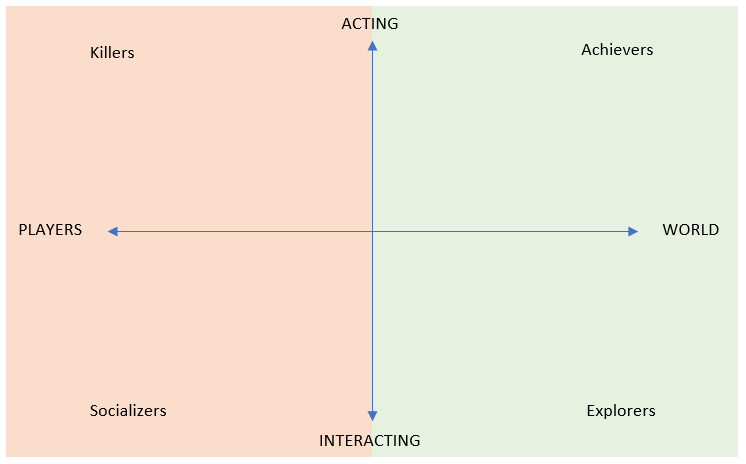
\includegraphics[width=0.75\textwidth, keepaspectratio]{Bilder/Diagramme/InterestGraphBartleAchieversExplorers.png}
	\caption{Benutzeroberfläche Fortschritts-Management}
	\label{img:interestGraphBartleAchiversExplorers}
\end{figure}

\par Durch den vorgesehenen Kontext der Applikation, die Studierenden während der Bearbeitung der Bachelorarbeit wegweisend zu unterstützen und zu motivieren, bietet sich somit an, Herausforderungen und die damit verbundenen Achievements in Form von kontextbezogenen fokuslenkenden Game-Design-Elementen (siehe \ref{sec:grundlagenkapitelGamification}) in die Applikation als festen Bestandteil der Motivationsstrategie zu integrieren.

\par\medskip Wie in \citep{Sailer2016}[S. 32 - 34] beschrieben wird, besitzen Achievements verschiedene Eigenschaften, die in Bezug auf Zielstellungen einer steuernden und in diesem Sinne auch fordernden Funktion dienen können. Ein wichtiges Kriterium bei der Wahl der Achievements als Spiel-Design-Elemente ist, dass sie dem Benutzer ein nicht-kontrollierendes, positives Feedback geben und somit nicht unangenehm kontrollieren oder den ohnehin schon sehr hoch ausfallenden Druck auf die Studierenden bei der Bearbeitung der Bachelorarbeit erhöhen. Es sollte in diesem Sinne nicht aus den Augen verloren werden, dass die Applikation den Studierenden positiv unterstützen soll.

\par\medskip Im weiteren Verlauf werden, den Nutzergruppen entsprechend, auf Spiel-Design-Elemente wie Bestenlisten oder andere soziale Motivationsmodelle verzichtet.

\par Weiterhin wird das Integrieren eines Punkte- oder Level-Systems sowie einer Avatar-Funktion nicht verfolgt. Dies dient der Absicht, dass die Applikation zwar motivierende Spiel-Design-Elemente enthalten soll, jedoch in einem Umfang, der keine an Gamification desinteressierten Benutzer ausschließen und somit in diesem Fall weiterhin eine brauchbare Hilfestellung bieten soll.

\newpage
\subsection{Übersicht der abgeleiteten Produktfunktionen und Anforderungen} \label{sub:produktfunktionen}
\par Im folgenden Verlauf sind die aus der Aufgabenstellung und der Anforderungsanalyse erhobenen Produktanforderungen in natürlicher Sprache vorzufinden. Diese wurden an einer Anforderungsschablone aus dem Lehrbuch der Softwaretechnik von Helmut Balzert orientiert \citep[Kapitel 19 - Natürlichsprachliche Anforderungen, Seite 481]{Balzert2010} und nach Bedarf spezifiziert:\\

\begin{enumerate} [label=\textbf{PR\arabic*}]

\item \label{prod:pZeitFortschritt} \textbf{Unterstützung bei Zeit- und Fortschrittsmanagement}
\begin{enumerate} [label=\textit{[Req1.\arabic*]}]
\item \label{anf:meilensteinVerwalten} Die Software muss den Studierenden ermöglichen, Meilensteine zu verwalten.
\begin{enumerate} [label=\textit{[Req1.1.\arabic*]}]
\item \label{uanf:meilensteinAnlegen} Das Anlegen von Meilensteinen
\item \label{uanf:meilensteinEntfernen} Das Entfernen von Meilensteinen
\item \label{uanf:meilensteinAendern} Das Ändern von Meilensteinen
\item \label{uanf:meilensteinVerschieben} Das Verschieben von Meilensteinen
\end{enumerate}

\bigskip
\item \label{anf:arbeitspaketVerwalten} Die Software muss dem Studierenden ermöglichen, dem Meilensteinen zugehörige Aufgaben zu verwalten.
\begin{enumerate} [label=\textit{[Req1.2.\arabic*]}]
\item \label{uanf:arbeitspaketAnlegen} Das Anlegen von Aufgaben
\item \label{uanf:arbeitspaketEntfernen} Das Entfernen von Aufgaben
\item \label{uanf:arbeitspaketAendern} Das Ändern von Aufgaben
\item \label{uanf:arbeitspaketMarkieren} Das Markieren von Aufgaben als \textit{abgeschlossen}
\end{enumerate}

\bigskip
\item \label{anf:erinnerungenBenachrichtigungen}Die Software soll die Studierenden auf bevorstehende Meilensteine und Aufgabenpakete aufmerksam machen.

\begin{enumerate} [label=\textit{[Req1.3.\arabic*]}]
\item \label{uanf:erinnerungAusloesen}Das Auslösen von Erinnerungen/Benachrichtigungen
\end{enumerate}
\end{enumerate}

\newpage
\item \label{prod:unterstuetzungBachelorarbeit} \textbf{Unterstützung bei der Bearbeitung der Bachelorarbeit}.

\begin{enumerate} [label=\textit{[Req2.\arabic*]}]
\item \label{anf:informationsTool} Die Software muss den Studierenden allgemeine Informationen zur Bearbeitung der Bachelorarbeit bereitstellen.

\begin{enumerate}[label=\textit{[Req2.1.\arabic*]}]
\item \label{anf:infRahmenbedingungenFormalien} Die Software muss den Studierenden Informationen über die Rahmenbedingungen und Formalien der Bachelorarbeit an der Fachhochschule Lübeck bereitstellen können.

\item \label{anf:infAufbauStruktur} Die Software muss den Studierenden Hinweise und Empfehlungen zu Aufbau und Struktur von Bachelorarbeiten bereitstellen können.

\item \label{anf:infDurchfuerungBachelorarbeit} Die Software muss den Studierenden Hinweise und Empfehlungen zur Durchführung von Bachelorarbeiten bereitstellen können.
\end{enumerate}

\bigskip
\item \label{anf:infMethodenTechniken} Die Software muss den Studierenden eine Übersicht über studiengang-spezifische und -übergreifende relevante Techniken und Methoden bereitstellen können.

\begin{enumerate} [label=\textit{[Req2.4.\arabic*]}]
\item \label{uanf:infThemenfindung} Hilfestellung/Übersicht zu Themenfindung für Bachelorarbeit
\item \label{uanf:infInhalt} Hilfestellung/Übersicht von studiengang-spezifischen Inhalten
\item \label{uanf:infAufbereitungErgebnisse} Hilfestellung/Übersicht zu Aufbereitung von Ergebnissen
\item \label{uanf:infNachweisfuerung} Hilfestellung/Übersicht zu Nachweisführung
\end{enumerate}

\bigskip
\item \label{anf:anpassungZielgruppen} Die Software muss den Umgang von zielgruppenspezifischen Anpassungen der Inhalte ermöglichen können.

\bigskip
\item \label{anf:anpassungSoftwareextern} Die Anpassungen der Inhalte soll software-extern realisierbar und integrierbar sein.
\end{enumerate}

\item\label{prod:gamificationelementeEinsatz} \textbf{Einsatz von Gamification-Elementen zur Steigerung der Motivation}
\begin{enumerate} [label=\textit{[Req3.\arabic*]}]
\item \label{anf:spielDesignElementeBenutzerklassen} Die Software muss im Rahmen der Gamification-Strategie Spiel-Design-Elemente bereitstellen, die den ermittelten Benutzerklassen entsprechen.

\bigskip
\item \label{anf:spielDesignElementeOrientiertungAnBachelorarabeit} Die Spiel-Design-Elemente sollen unter Berücksichtigung der wegweisenden Eigenschaft geeignet an dem Ablauf einer Bachelorarbeit orientiert sein.
\end{enumerate}

\bigskip
\item \textbf{\label{prod:sonstige} Weitere Anforderungen}
\begin{enumerate} [label=\textit{[Req4.\arabic*]}]
\item \label{anf:mehrsprachig} Die Software muss sämtliche Inhalte und Leistungen auch für fremdsprachige Personengruppen enthalten.

\bigskip
\item \label{anf:persoenlicheThemenvorschlaege} Die Software kann die Möglichkeit bieten, dass Betreuer ihre persönlichen Themenvorschläge für die Studierenden sichtbar per Weboberfläche hinzufügen/entfernen können 
\end{enumerate}


\end{enumerate}

\newpage
\subsection{Übersicht der Risiken} \label{sub:risikouebersicht}
\par Im Laufe der mit den Professoren durchgeführten Interviews wurden häufig Bedenken bezüglich der Risiken geäußert, die der Einsatz der Software für die Studierenden mit sich bringen könnte. 
\par \bigskip Es folgt die Aufzählung der ermittelten Risiken sowie einer Gewichtung in Bezug auf die Stärke der negativen Auswirkungen bei Eintreten dieser Risiken:

\begin{enumerate} [label=\textit{[R\arabic*]}]
\item \label{risk:realerZustand} 
\par Auswirkungen: Hoch
\par Die Applikation kennt den realen Zustand und Fortschritt der Bachelorarbeit nicht und könnte somit zu einer Verfälschung des realen Bildes führen. Studierende könnten somit den eigentlichen Zustand der Arbeit aus den Augen verlieren.
\item \label{risk:inhaltUnumstoesslich} 
\par Auswirkungen: Hoch
\par Studierende könnten die Hilfestellung der Applikation als unumstößlich ansehen und so unter Umständen in Konflikt mit dem Betreuer kommen.
\item \label{risk:erstazBetreuer} 
\par Auswirkungen: Hoch
\par Die Applikation kann als Ersatz für die Betreuung von einem Professor oder einer Professorin wahrgenommen werden, was zu weitreichenden Konsequenzen für die Qualität der Abschlussarbeit führen könnte.
\item \label{risk:keinLerneffekt} 
\par Auswirkungen: Hoch
\par Durch die Nutzung der Applikation wird dem Studierenden so viel Arbeit abgenommen, dass der Lerneffekt der Bachelorarbeit zu gering ist.
\item \label{risk:ueberplanung} 
\par Auswirkungen: Mittel
\par Die Applikation könnte im Rahmen des Zeitmanagement-Tools zu einer Überplanung führen, was den Studierenden von der eigentlichen Arbeit abhalten könnte.
\item \label{risk:gamificationEffekt} 
\par Auswirkungen: Gering
\par Gamification-Elemente können einen sehr geringen Effekt haben, da nicht sie die Motivation aufrechterhalten, sondern das Interesse des Studierenden.
\end{enumerate}

\newpage
\subsection{Übersicht der Chancen} \label{sub:chancenuebersicht}
\par Aus den gewonnen Informationen, die sich aus dem Verlauf der Interviews mit den Professoren und der schriftlichen Befragung mit den Studierenden ergeben haben, ließen sich Chancen für Betreuer und Studierende durch Einsatz der Applikation identifizieren, welche im Folgenden genannt werden.

\par \bigskip Es folgt die Aufzählung der ermittelten Chancen sowie einer Gewichtung in Bezug auf die Stärke der positiven Auswirkungen bei Erreichen dieser Chancen:

\begin{enumerate} [label=\textit{[C\arabic*]}]
\item 
\par Auswirkungen: Hoch
\par Aufnahmebereitschaft gegenüber Tipps, Empfehlungen und anderen Aspekten könnte im Gegensatz zum Bachelorarbeit-Seminar gesteigert werden, da der Einsatz der Applikation von begleitender Natur ist und sich die Studierenden somit besser mit dem Problem identifizieren könnten.
\item
\par Auswirkungen: Hoch
\par Vermeiden von großen Fehlern durch Lenken des Fokus der Studierenden auf wichtige Aspekte der Bachelorarbeit, bei denen üblicherweise häufig Probleme auftreten.
\item
\par Auswirkungen: Hoch
\par Besseres Zeitmanagement der Studierenden und die Steigerung der organisatorischen Fähigkeiten durch Anwendung der Applikation.
\item
\par Auswirkungen: Hoch
\par Systematischere Vorgehensweise der Studierenden bei Problemanalyse, Anforderungserhebung und Nachweisführung
\item
\par Auswirkungen: Hoch
\par Senken des Beratungsaufwandes seitens der Betreuer bei Trivialitäten und bei sich wiederholenden Fragestellungen.
\item 
\par Auswirkungen: Mittel
\par Neuer Informationskanal für Studierende, welcher Wissenslücken bezüglich der Rahmenbedingungen und Regeln einer Bachelorarbeit schließen kann.
\item
\par Auswirkungen: Mittel
\par Zielgerichteterer Methoden- und Werkzeugeinsatz sowie Anwendung fachspezifischer und fachübergreifender Techniken.
\item
\par Auswirkungen: Mittel
\par Minimieren von Problemen bei der Gestaltung der Dokumentation.
\item
\par Auswirkungen: Gering
\par Bessere Vorbereitung der Studierenden auf Gesprächstermine mit dem Betreuer.
\end{enumerate}

\newpage
\chapter{Konzeptvorstellung der Applikation} \label{chap:konzept}

\section{Beschreibung der Software}
\par Die zu entwickelnde Applikation kann in verschiedene Kern-Softwareabschnitten unterteilt werden. Diese Abschnitte lassen sich weiterhin auf folgende namensgebende Aufgabenbereiche aufteilen, welche sich an den erhobenen Anforderungen und der Aufgabenstellung orientieren (siehe Kapitel \ref{sub:produktfunktionen}).

\begin{itemize}
\item Meilensteinverwaltung
\item Bachelorarbeit Guide
\item Herausforderungen
\item Achievements
\item Dashboard
\item Sonstige Softwareinhalte
\end{itemize}

\newpage
\subsection{Meilensteinverwaltung}
\par Die Meilensteinverwaltung ist eine Funktion, die das Anlegen, Planen und Verwalten von Meilensteinen sowie der zugehörigen Unteraufgaben ermöglichen soll. 
\par Ferner soll die Meilensteinverwaltung nicht den detaillierten Prozess des gesamten Projektmanagements abbilden, sondern die Aufgabe der übersichtlichen Handhabung von Unteraufgaben und Verdeutlichung von Fristen in Form einer dynamischen ToDo-Listenverwaltung unterstützen. Hierbei soll dem Anwender weiterhin die größtmögliche Freiheit der Gestaltung des Plans zukommen, um individuelle Arbeitsweisen zu berücksichtigen. 
\par \bigskip Der im Projektmanagement definierte Begriff \grqq Meilenstein\grqq{} bezeichnet hierbei einen Zeitpunkt, zu welchem der vom Nutzer definierte Arbeitsstand erreicht sein soll.

\par\bigskip Es folgt eine stichpunktartige Auflistung und Beschreibung der Kernfeatures des Tools:
\begin{itemize}
\item \textbf{Erstellung und Verwaltung von Meilensteinen}
\par Es können Meilensteine erstellt \ref{uanf:meilensteinAnlegen}, bearbeitet\ref{uanf:meilensteinAendern}, verschoben\ref{uanf:meilensteinVerschieben} und entfernt\ref{uanf:meilensteinEntfernen} werden. 
\item \textbf{Erstellung und Verwaltung von Unteraufgaben}
\par Jeder Meilenstein enthält optionale Unteraufgaben\ref{anf:arbeitspaketVerwalten}, die von dem Benutzer einem Meilenstein hinzugefügt\ref{uanf:arbeitspaketAnlegen}, bearbeitet\ref{uanf:arbeitspaketAendern} und gelöscht\ref{uanf:arbeitspaketEntfernen} werden können. Weiterhin lassen sich die Unteraufgaben als \textit{abgeschlossen} markieren\ref{uanf:arbeitspaketMarkieren}, um dem Benutzer die Möglichkeit zu bieten, seine Aufgaben zu organisieren.
\end{itemize}

\bigskip
\begin{figure}[H]
	\centering
	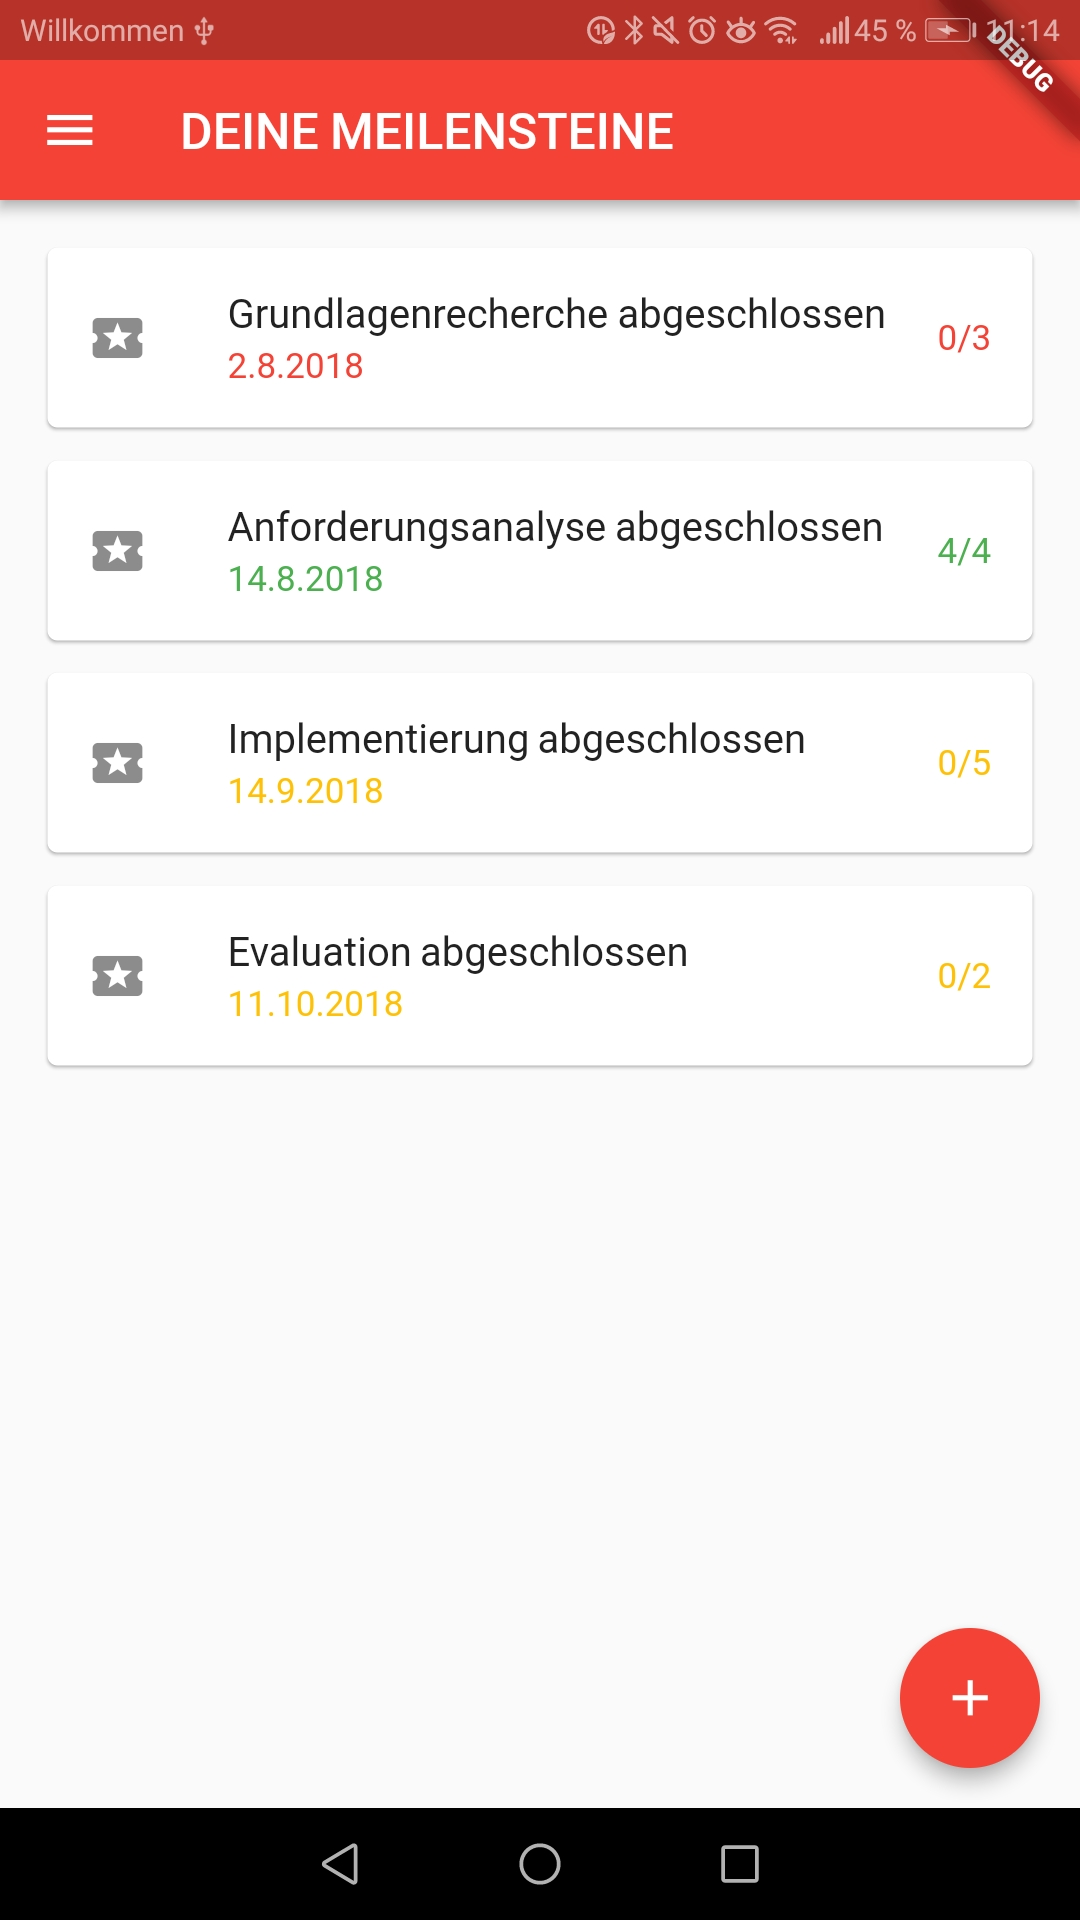
\includegraphics[width=0.35\textwidth, keepaspectratio]{Bilder/Prototyp/app_screenshots/MeilensteinOverviewScreenshot.jpg}
	\caption{Benutzeroberfläche Meilensteinverwaltung}
	\label{img:fortschrittsmanagement}
\end{figure}

\newpage
\subsection{Bachelorarbeit Guide}
\par Der Guide stellt den Teil der Applikation dar, der die Bereitstellung von Hinweisen, Tipps und weiteren hilfreichen Informationen zur Bearbeitung der Bachelorarbeit abdecken soll. Dieser Inhalt ergibt sich aus der Verwendung des von der Fachhochschule Lübeck ausgehändigten Dokuments, welches als Ratgeber bei der Erstellung von Bachelorarbeiten funktionieren und somit die speziellen Anforderungen der Fachhochschule Lübeck berücksichtigen soll \citep[vgl. Kapitel 1]{FHLuebeckBAAnleitung}.
\par \bigskip In dieser Hinsicht soll der Guide als genereller Anlaufpunkt fungieren, der eine Hilfestellung für Bacheloranden darstellt\ref{anf:infMethodenTechniken}.

\par\bigskip Die Bandbreite der Hinweise, Tipps und weiteren Informationen sollen somit den gesamten Verlauf der Bachelorarbeit abdecken und lässt sich in diesem Zusammenhang in folgende Bereiche und Inhalte zerlegen, welche sich an dem genannten Leitfaden der Fachhochschule Lübeck zur Erstellung einer Bachelorarbeit orientieren.

\bigskip
\begin{figure}[H]
\centering
	\subfigure[Guide Hauptbildschirm]{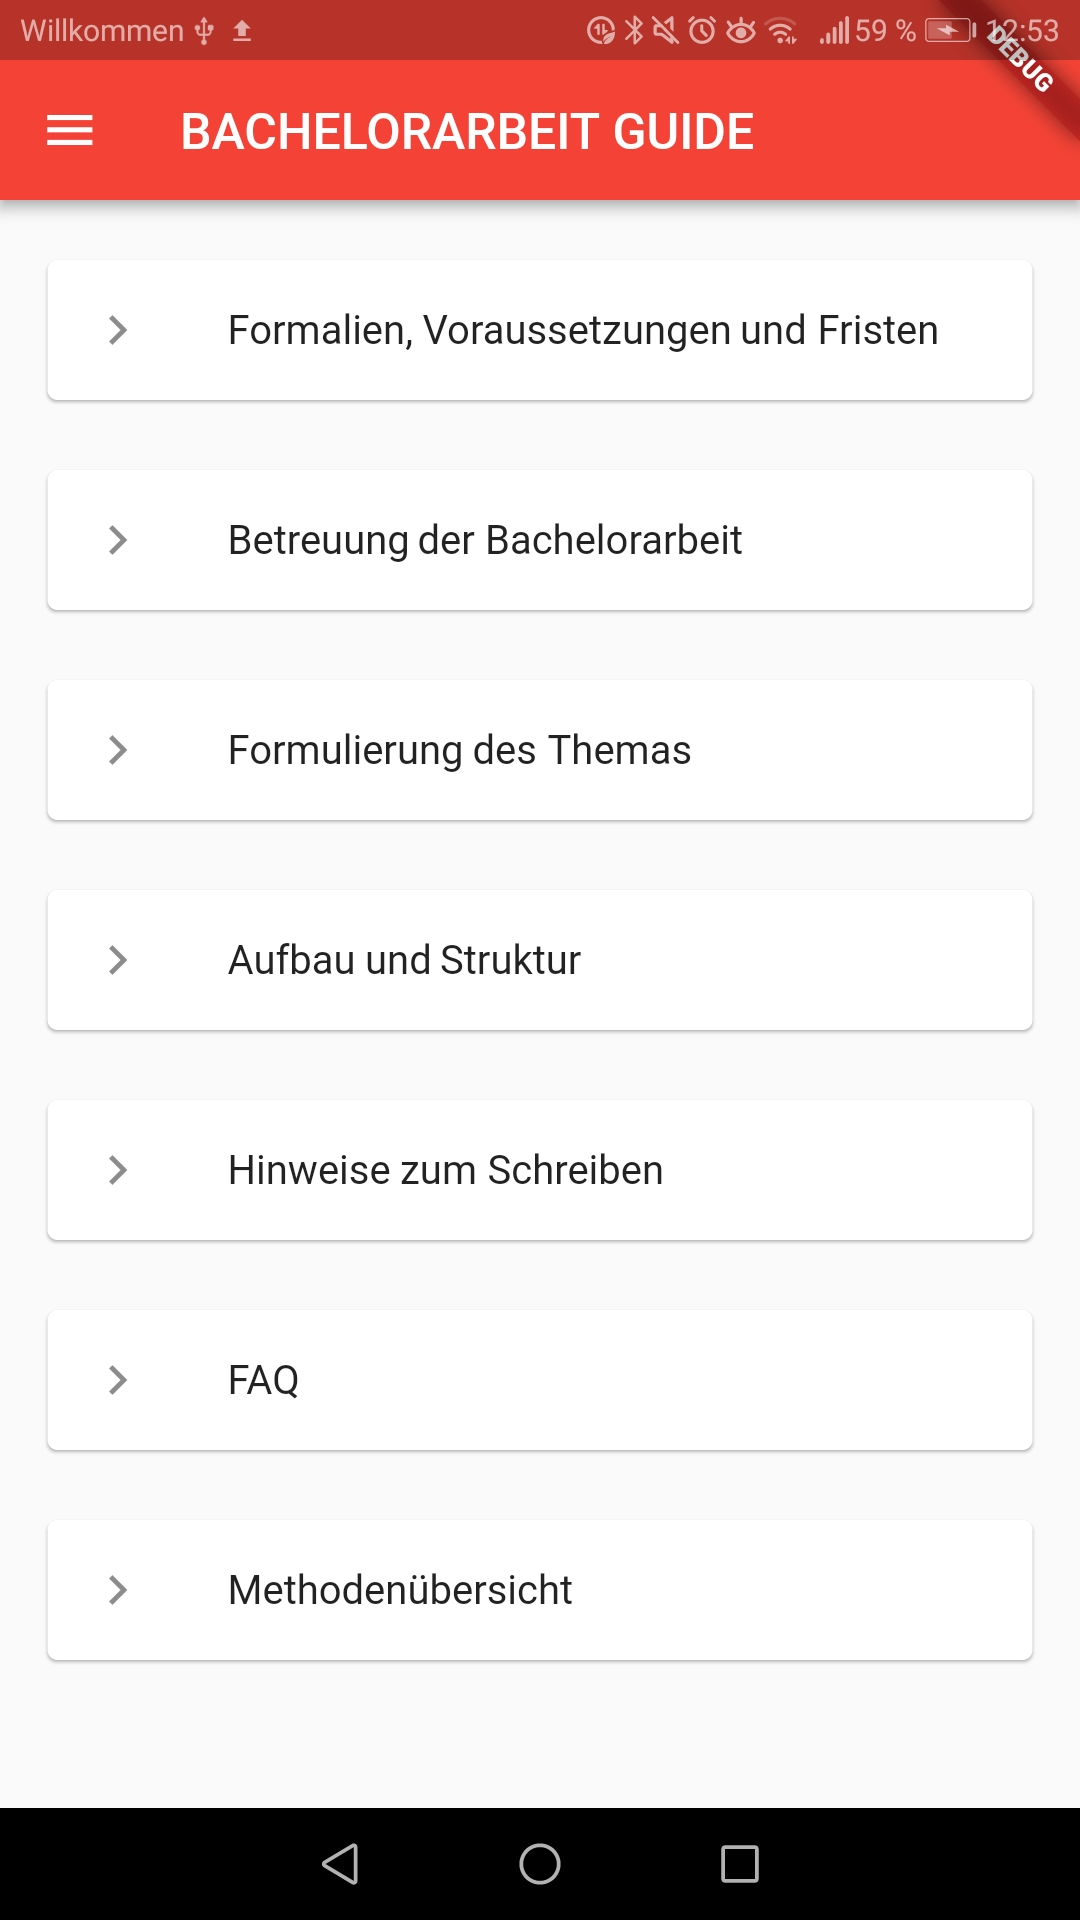
\includegraphics[width=0.35\textwidth]{Bilder/Prototyp/app_screenshots/BachelorGuideOverview.jpg}}
	\subfigure[Guide Themen-Ebene]{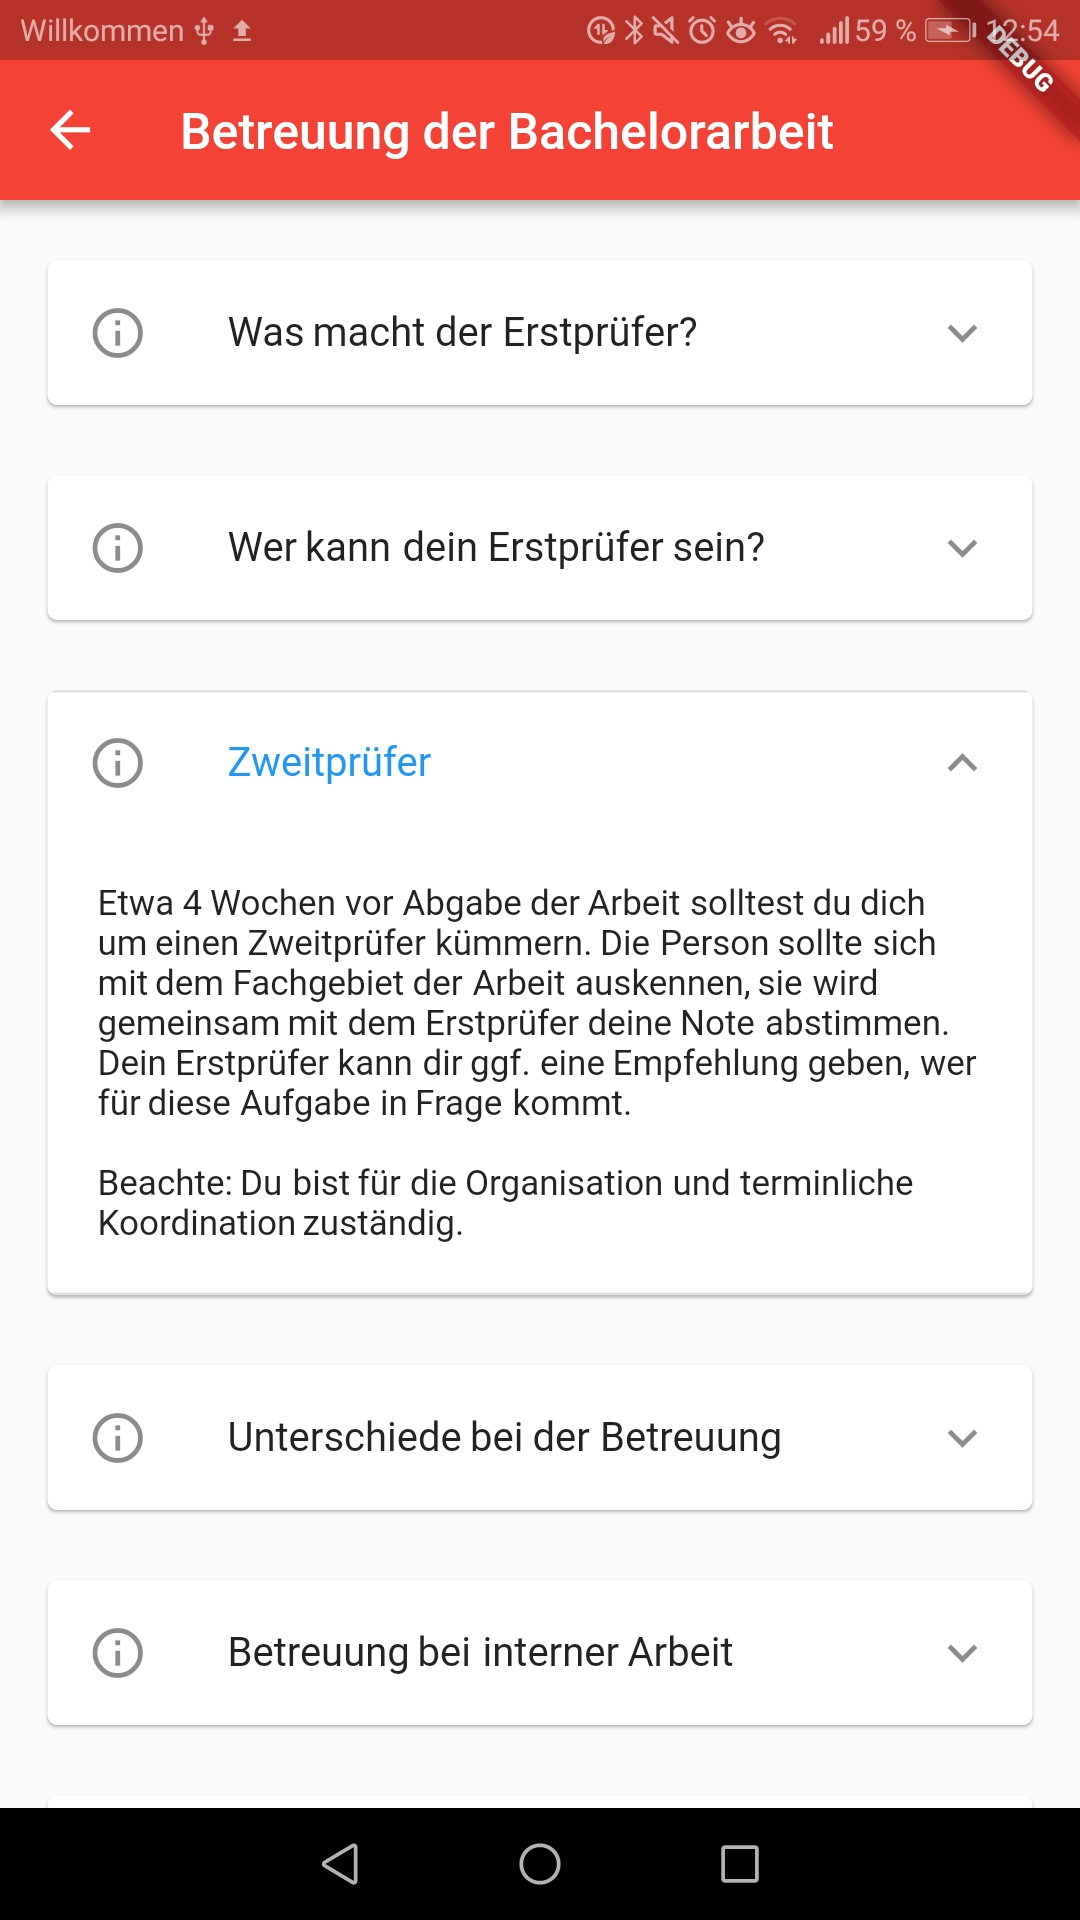
\includegraphics[width=0.35\textwidth]{Bilder/Prototyp/app_screenshots/BachelorGuideDetails.jpg}}
	\caption{Benutzeroberfläche Guide}
	\label{img:guide}
\end{figure}

\newpage
\par\bigskip Es folgt eine Interpretation und Beschreibung der Unterteilung der Themengebiete:

\par\bigskip \textit{Anmerkung: Die folgenden Themengebiete stellen nur eine Möglichkeit der Aufteilung dar. Bei Einsatz der Software sollen die hier dargestellten Inhalte individuell erweitert oder verändert werden können(\ref{anf:anpassungZielgruppen}, \ref{anf:anpassungSoftwareextern}).}

\begin{itemize}
\item \textbf{Formalien, Voraussetzungen und Fristen}
\par Dieser Abschnitt beinhaltet die allgemeinen Informationen, die vor allem zur Klärung der Formalien bei der Bearbeitung der Abschlussarbeit wichtig sind.\ref{anf:infRahmenbedingungenFormalien}

\item \textbf{Formulierung des Themas}
\par In dieser Sektion befinden sich zahlreiche Tipps und hilfreiches Wissen zur Formulierung des eigenen Themas und der zu verfassenden Aufgabenstellung.

\item \textbf{Betreuung der Bachelorarbeit}
\par Informationen zur Betreuung von Bachelorarbeiten und was hinsichtlich des Engagements und der Vorgehensweise von den Studierenden erwartet wird, sind in diesem Abschnitt zu finden.

\item \textbf{Aufbau und Struktur}
\par Dieser Abschnitt befasst sich näher mit dem Aufbau der Bachelorarbeit und stellt vor allem Informationen und Empfehlungen bereit, welche sich auf die Strukturierung und die Bedeutung der einzelnen Kapitel der Bachelorarbeit beziehen.\ref{anf:infAufbauStruktur}

\item \textbf{Hinweise zum Schreiben}
\par In diesem Abschnitt werden tiefgehende Informationen und Empfehlungen behandelt, welche sich auf die praktische Umsetzung des Schreibens im Detail beziehen. Beispielhaft hierfür sind der Schreibstil, die Verwendung von Zeiten oder die Einbindung von Bildern, Tabellen und Programmcode.\ref{anf:infDurchfuerungBachelorarbeit}

\item \textbf{Methodenübersicht}
\par Dieser Abschnitt bietet eine Übersicht wichtiger Methoden der Informatik, die sich bei der Bearbeitung und Dokumentation der Bachelorarbeit als hilfreich erweisen könnten.\ref{anf:infMethodenTechniken}

\item \textbf{FAQ}
\par Dieses Kapitel behandelt oft gestellte Fragen und verdeutlicht die Informationen in der Form eines Frage-Antwort Schemas.
\end{itemize}

\newpage
\subsection{Herausforderungen}
\par Die sogenannten Herausforderungen\ref{anf:spielDesignElementeBenutzerklassen} sollen im Rahmen der Applikation, im Gegensatz zu den frei definierbaren Meilensteinen, eine fest definierte kategorisierte Aufteilung von typischen im Verlauf einer Bachelorarbeit zu leistenden Aufgaben darstellen\ref{anf:spielDesignElementeOrientiertungAnBachelorarabeit}. 
\par \bigskip Diese Aufgaben sollen vor allem als interaktiver Leitfaden dienen, an welchem sich die Studierenden orientieren können. Hierbei wird das Ziel angestrebt, den Studierenden eine Perspektive auf alle Phasen einer Bachelorarbeit sowie den jeweiligen einzelnen Arbeitsschritten zu geben, welche von den Studierenden abgehakt werden können.
\par \bigskip Durch die in der Anforderungsanalyse ermittelten Daten hat sich der Eindruck ergeben, dass viele Studierende gerade zu Beginn der Bearbeitungszeit dazu neigen, die Arbeit, aufgrund der noch viel verbleibenden Zeit, aufzuschieben. Unter diesem Aspekt wird hierbei versucht, durch das Abhaken von kleinen konkreten Aufgaben bereits frühzeitig einen fließenden Arbeitsablauf (Workflow) seitens der Studierenden anzustreben.

\par \bigskip \textit{Hinweis: Der Inhalt und Ablauf der dargestellten Herausforderungen ist im Rahmen der Prototypentwicklung lediglich beispielhaft erfolgt und stellt somit keinen korrekten und vollständigen Entwurf dar}

\bigskip
\begin{figure}[H]
\centering
	\subfigure[Herausforderungen - Roter Faden]{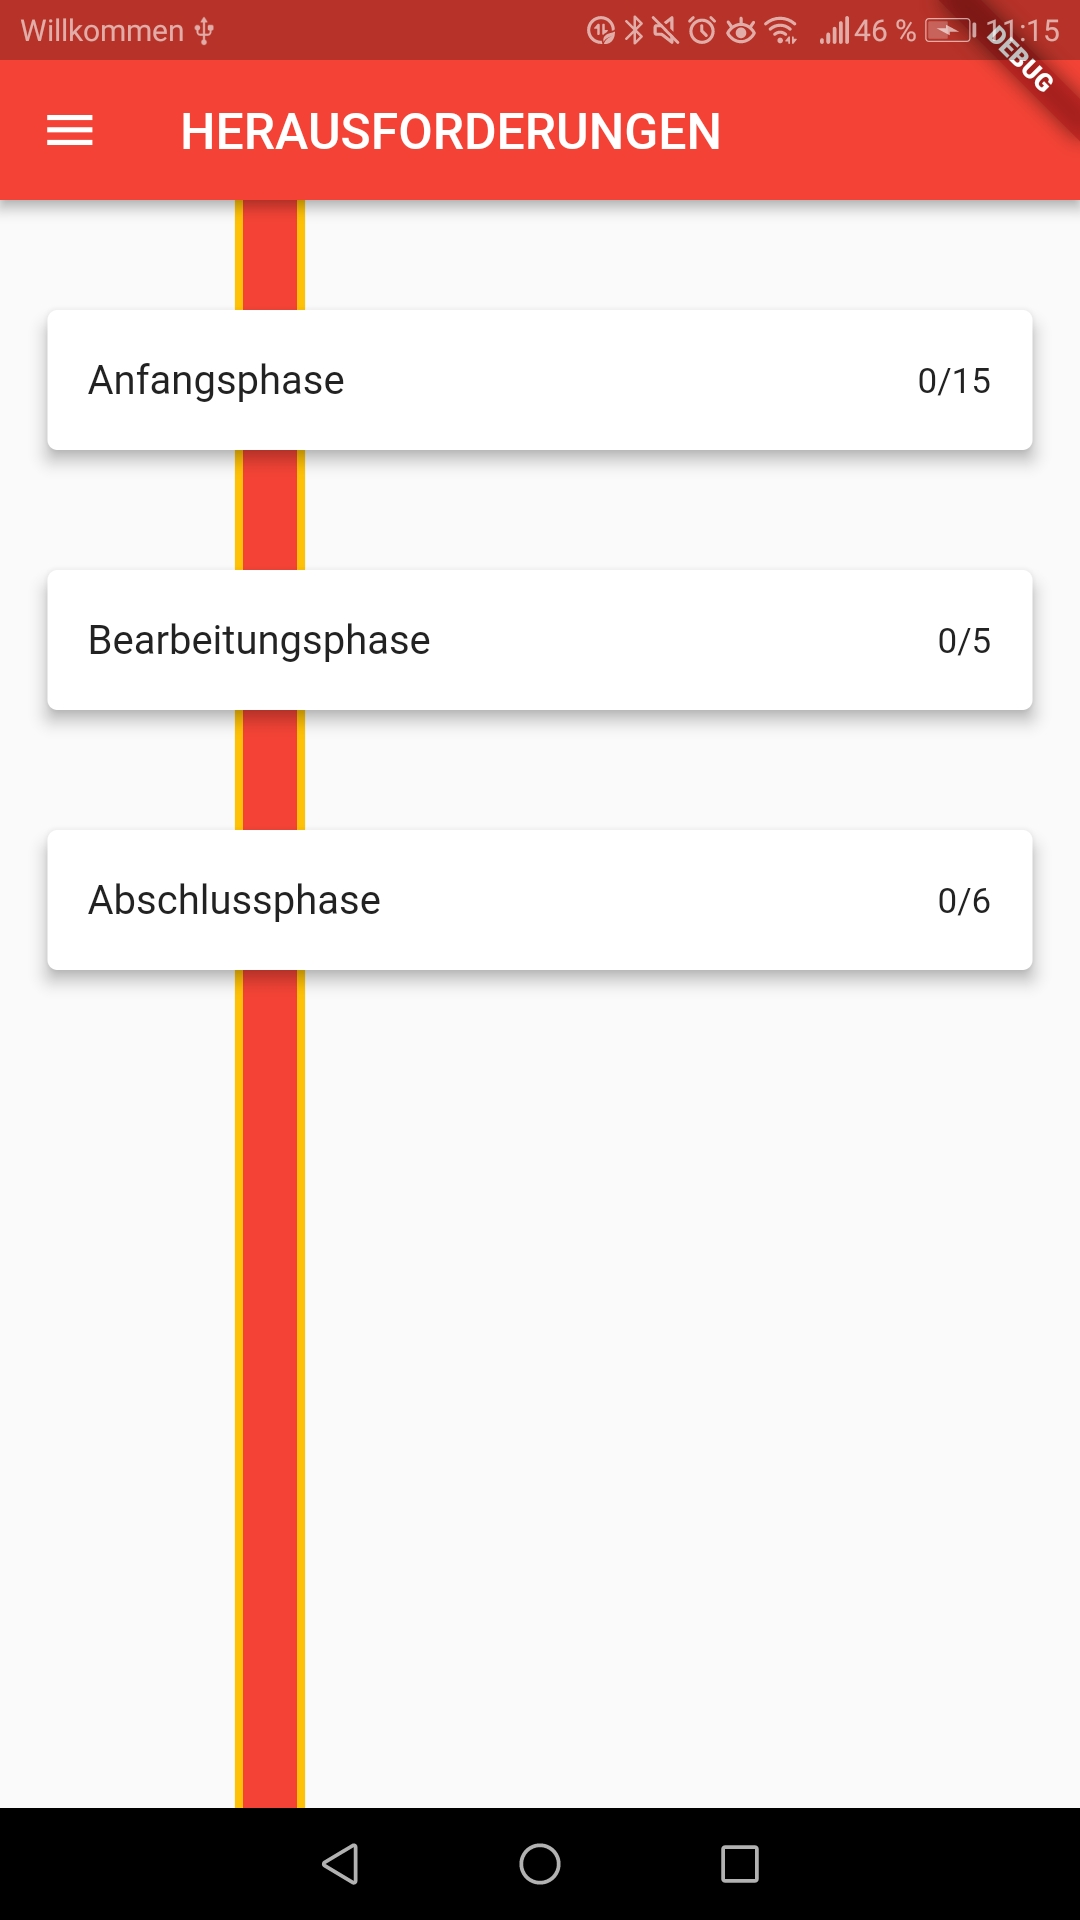
\includegraphics[width=0.35\textwidth]{Bilder/Prototyp/app_screenshots/HerausforderungenOverviewScreenshot.jpg}}
	\subfigure[Herausforderungen - Details]{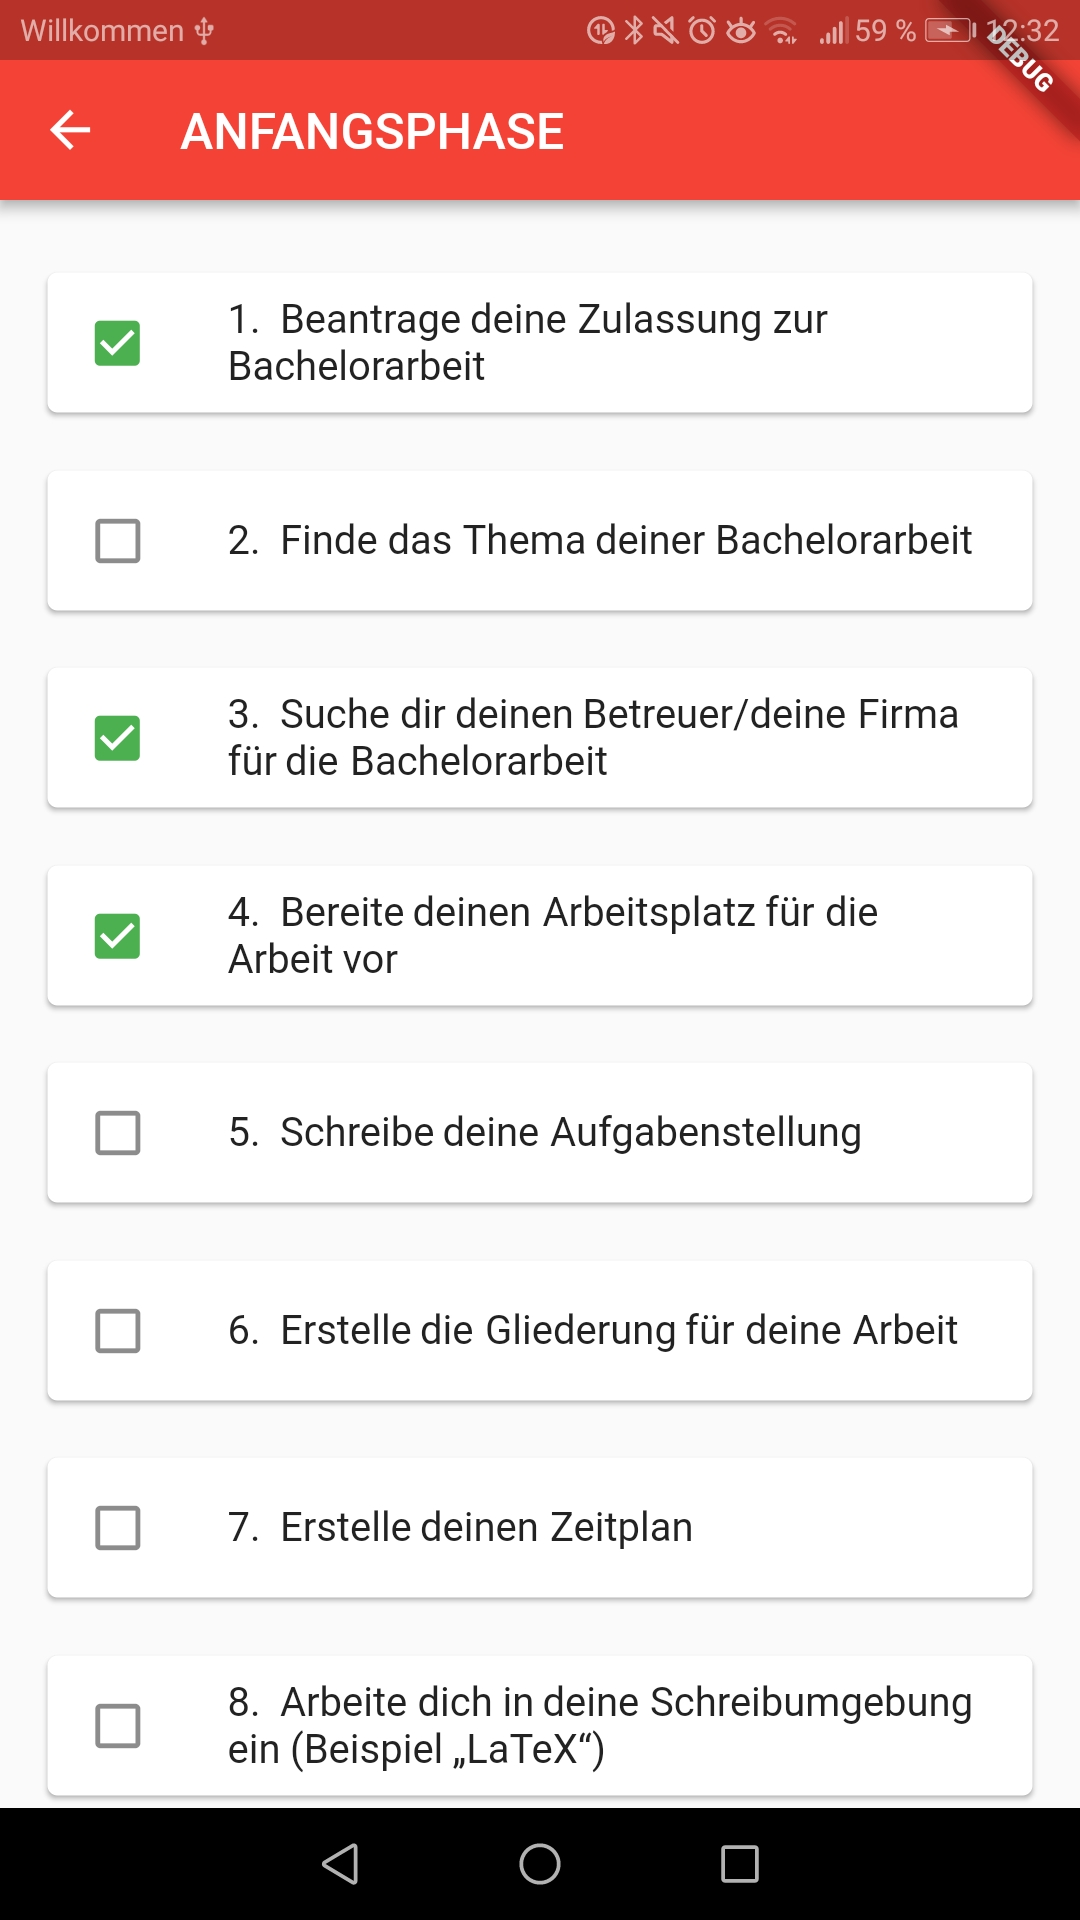
\includegraphics[width=0.35\textwidth]{Bilder/Prototyp/app_screenshots/HerausforderungenDetailsScreenshot.jpg}}
	\caption{Benutzeroberfläche Herausforderungen}
	\label{img:guide}
\end{figure}

\newpage
\subsection{Achievements}
\par Der Achievement-Hauptbildschirm\ref{anf:spielDesignElementeBenutzerklassen} enthält eine Übersicht der verschiedenen Kategorien von Achievements (siehe Abbildung \ref{img:achievements}). Die nächste Ebene dieses Abschnitts zeigt die detaillierte Ansicht der jeweiligen Achievements an, bei welcher der Benutzer einsehen kann, welche Achievements er bereits erhalten hat. 

\par \bigskip \textit{Hinweis: Weitere Informationen zu den einzelnen Achievements und deren Kategorien finden sich im Kapitel \ref{sec:gamificationelemente}.}

\bigskip
\begin{figure}[H]
\centering
	\subfigure[Achievements Hauptbildschirm]{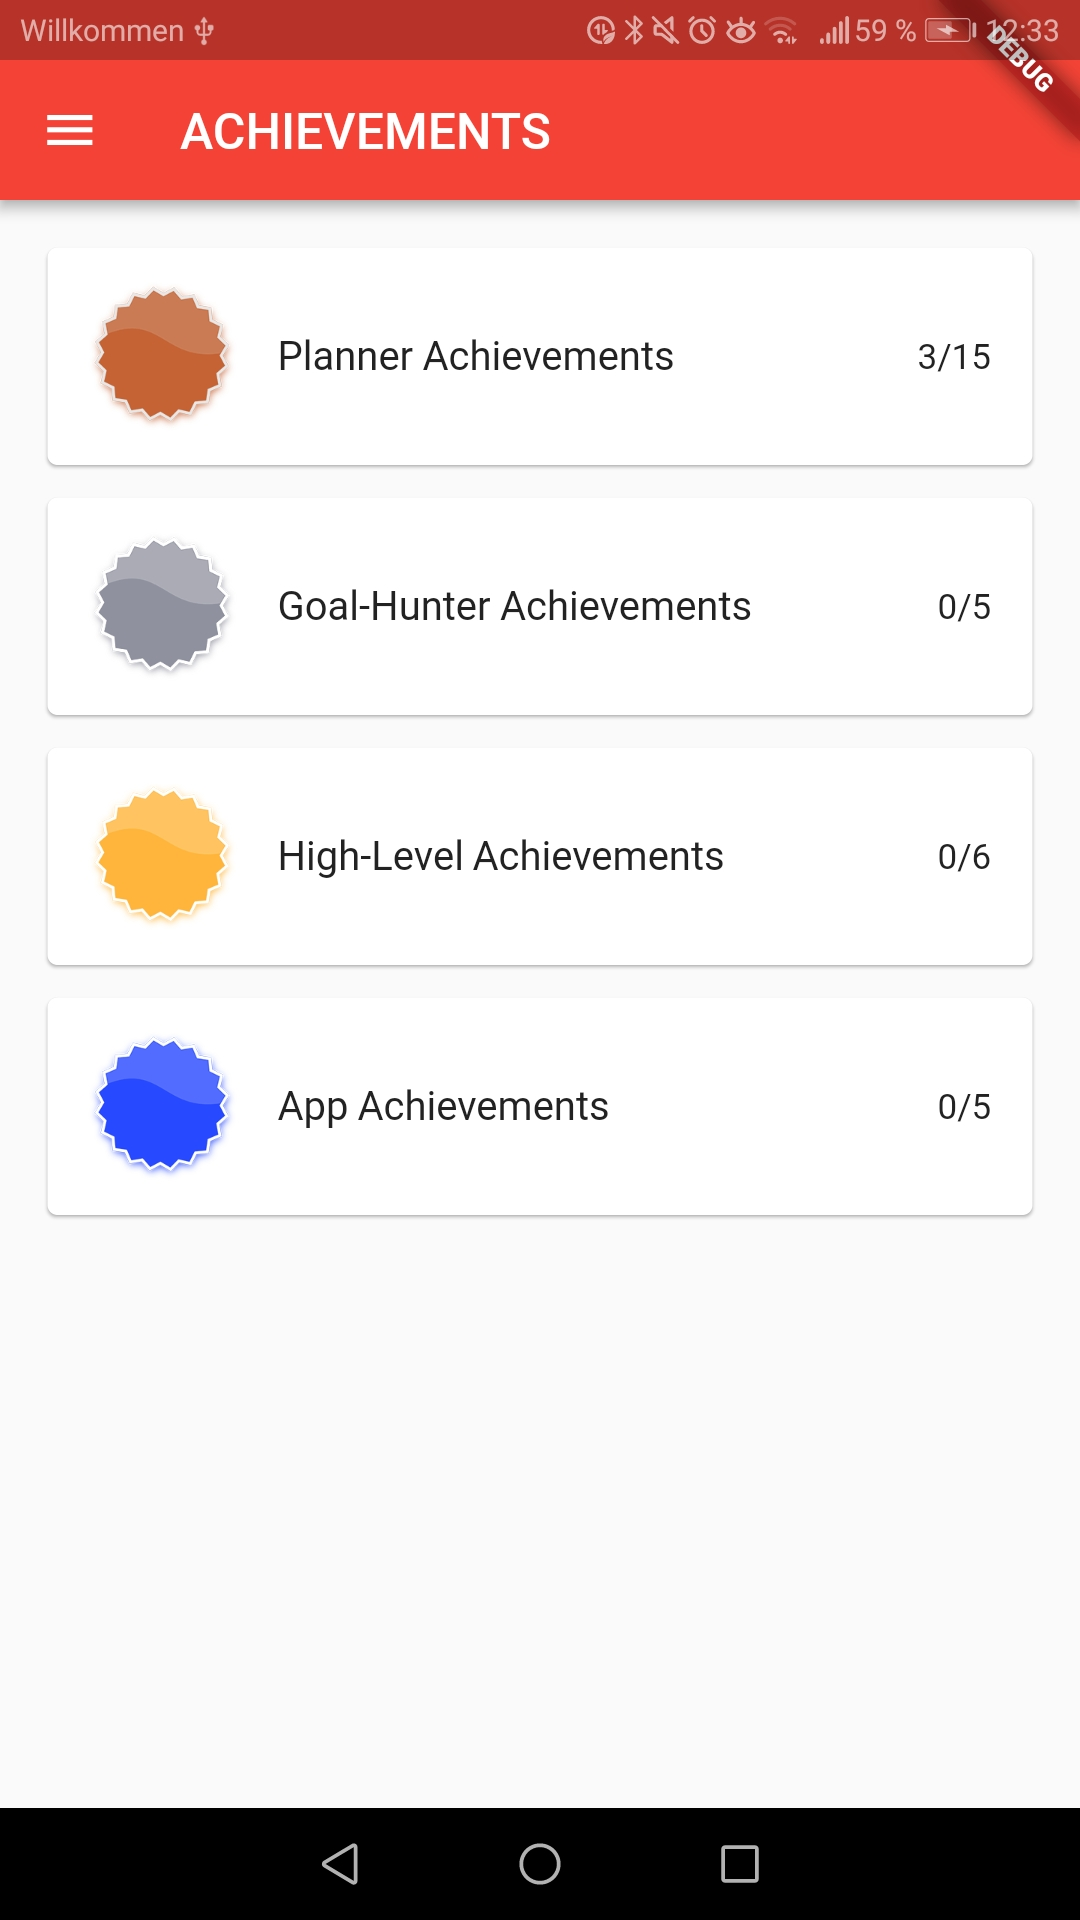
\includegraphics[width=0.35\textwidth]{Bilder/Prototyp/app_screenshots/AchievementsOverviewScreenshot.jpg}}
	\subfigure[Beispiel: Planner Achievements]{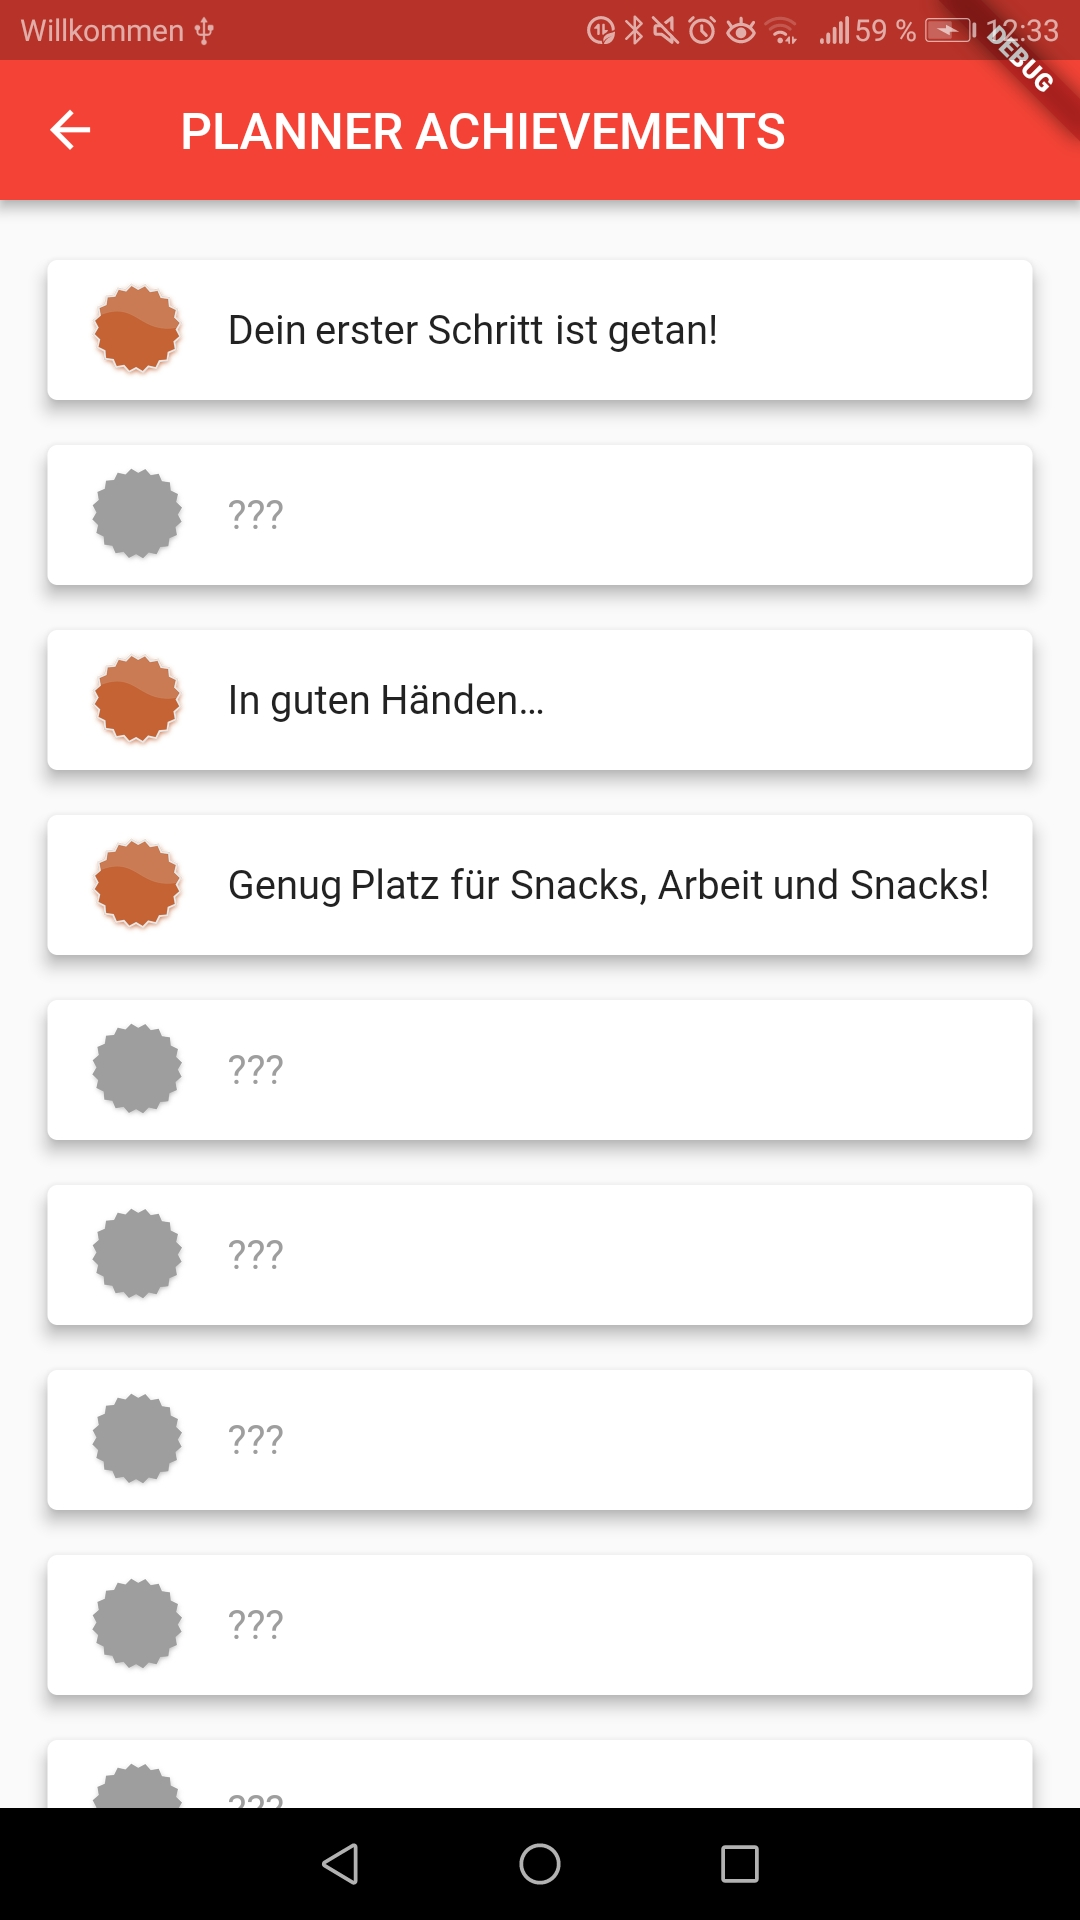
\includegraphics[width=0.35\textwidth]{Bilder/Prototyp/app_screenshots/AchievementsDetailsScreenshot.jpg}}
	\caption{Benutzeroberfläche Achievements}
	\label{img:achievements}
\end{figure}

\newpage
\subsection{Sonstige Softwareinhalte}
\par Über die eigentlichen individuellen Funktionalitäten hinaus sind weitere Grundfunktionalitäten vorhanden, welche unter den Punkt \textbf{Sonstige Softwareinhalte} fallen.

\par\medskip Es folgt eine stichpunktartige Auflistung und Beschreibung der Inhalte:
\begin{itemize}
\item \textbf{Menü}
\par Das Menü zeigt die existierenden Softwareabschnitte in einer klassisch gelisteten Menüstruktur (siehe Abbildung \ref{img:navigation}).
\item \textbf{Einstellungen}
\par Die Einstellungen beinhalten Optionen, die sich auf die Eigenschaften der Applikation auswirken, beispielsweise das Verändern des Designs oder der Sprache\ref{anf:mehrsprachig}
\end{itemize}

\bigskip
\begin{figure}[H]
	\centering
	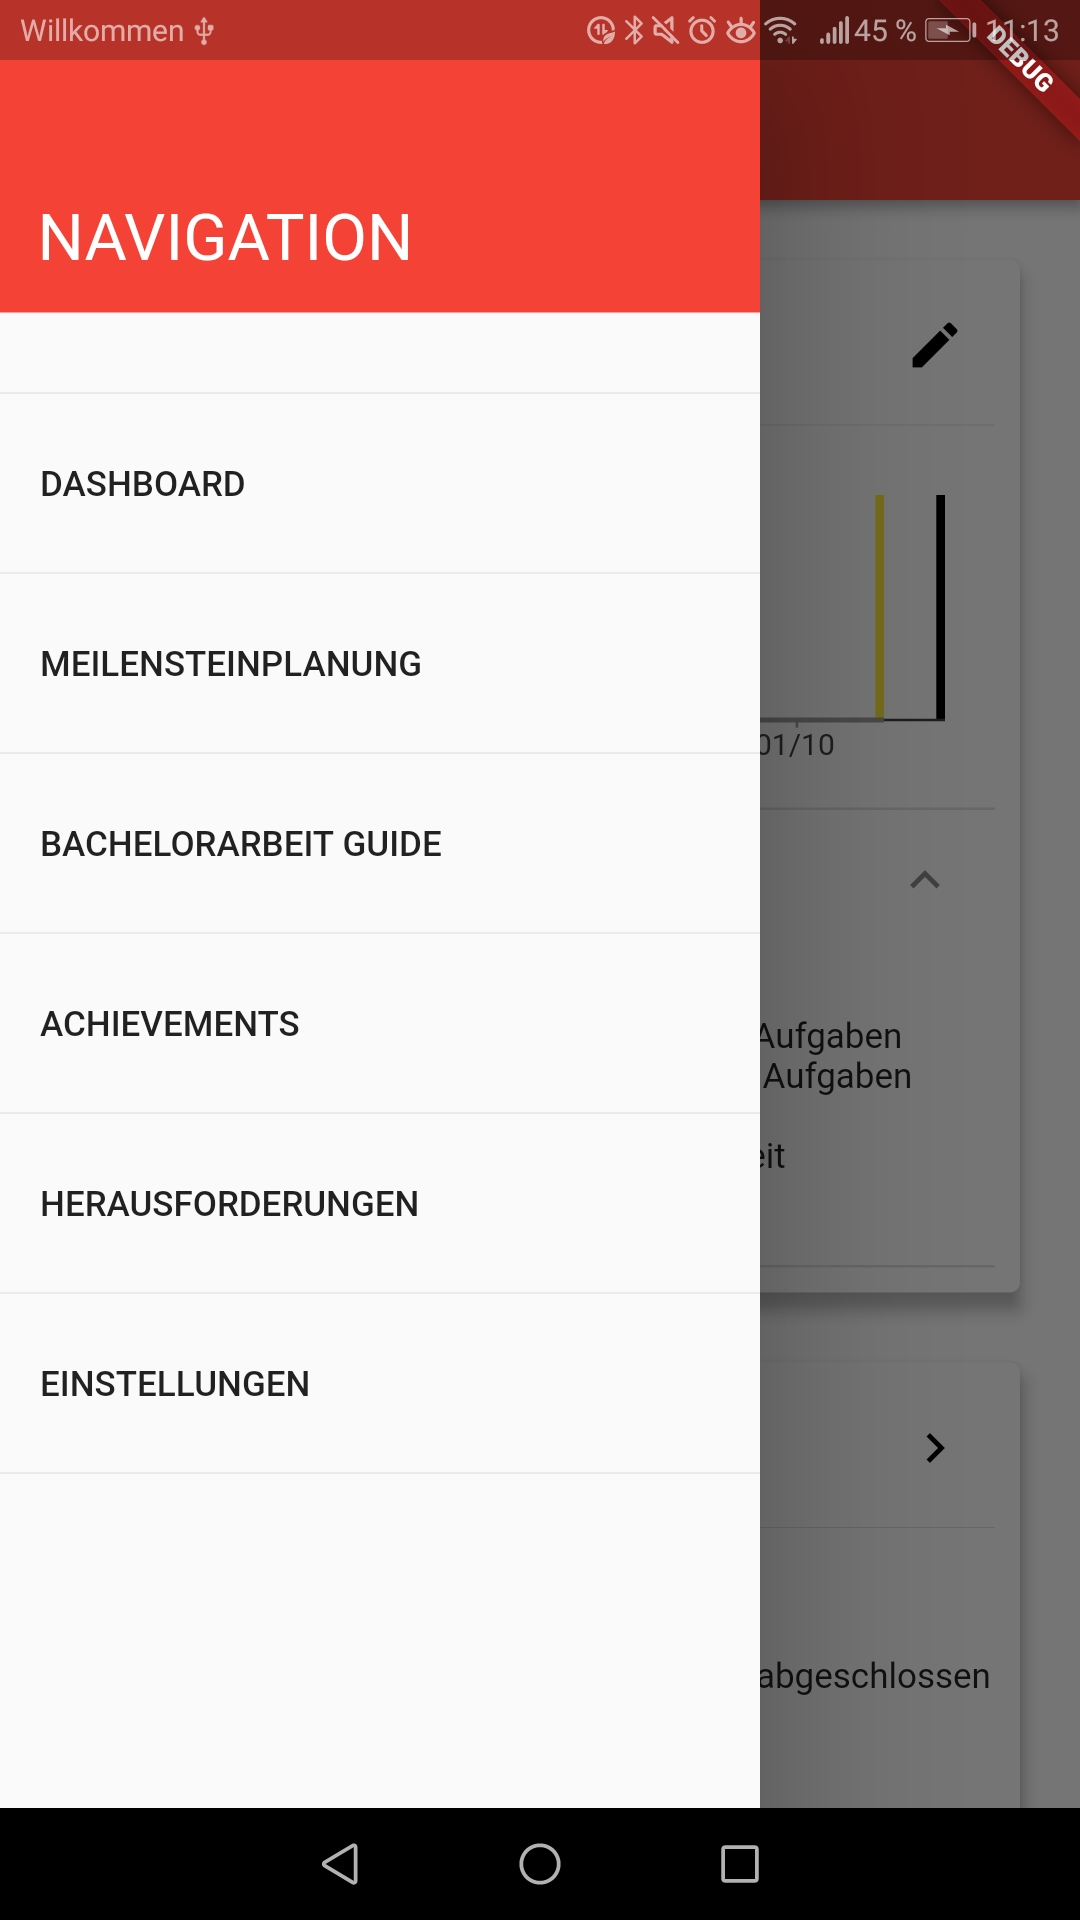
\includegraphics[width=0.4\textwidth,keepaspectratio]{Bilder/Prototyp/app_screenshots/MenuScreenshot.jpg}
	\caption{Benutzeroberfläche Navigations-Menü}
	\label{img:navigation}
\end{figure}

\newpage
\subsection{Dashboard}
\par Das Dashboard stellt den Ausgangspunkt und Hauptbildschirm der Applikation dar und trägt somit die Aufgabe, aktuelle Informationen für den Nutzer aufbereitet anzuzeigen und die verschiedenen Funktionen der Applikation im Bund darzustellen.

\bigskip
\begin{figure}[H]
	\centering
		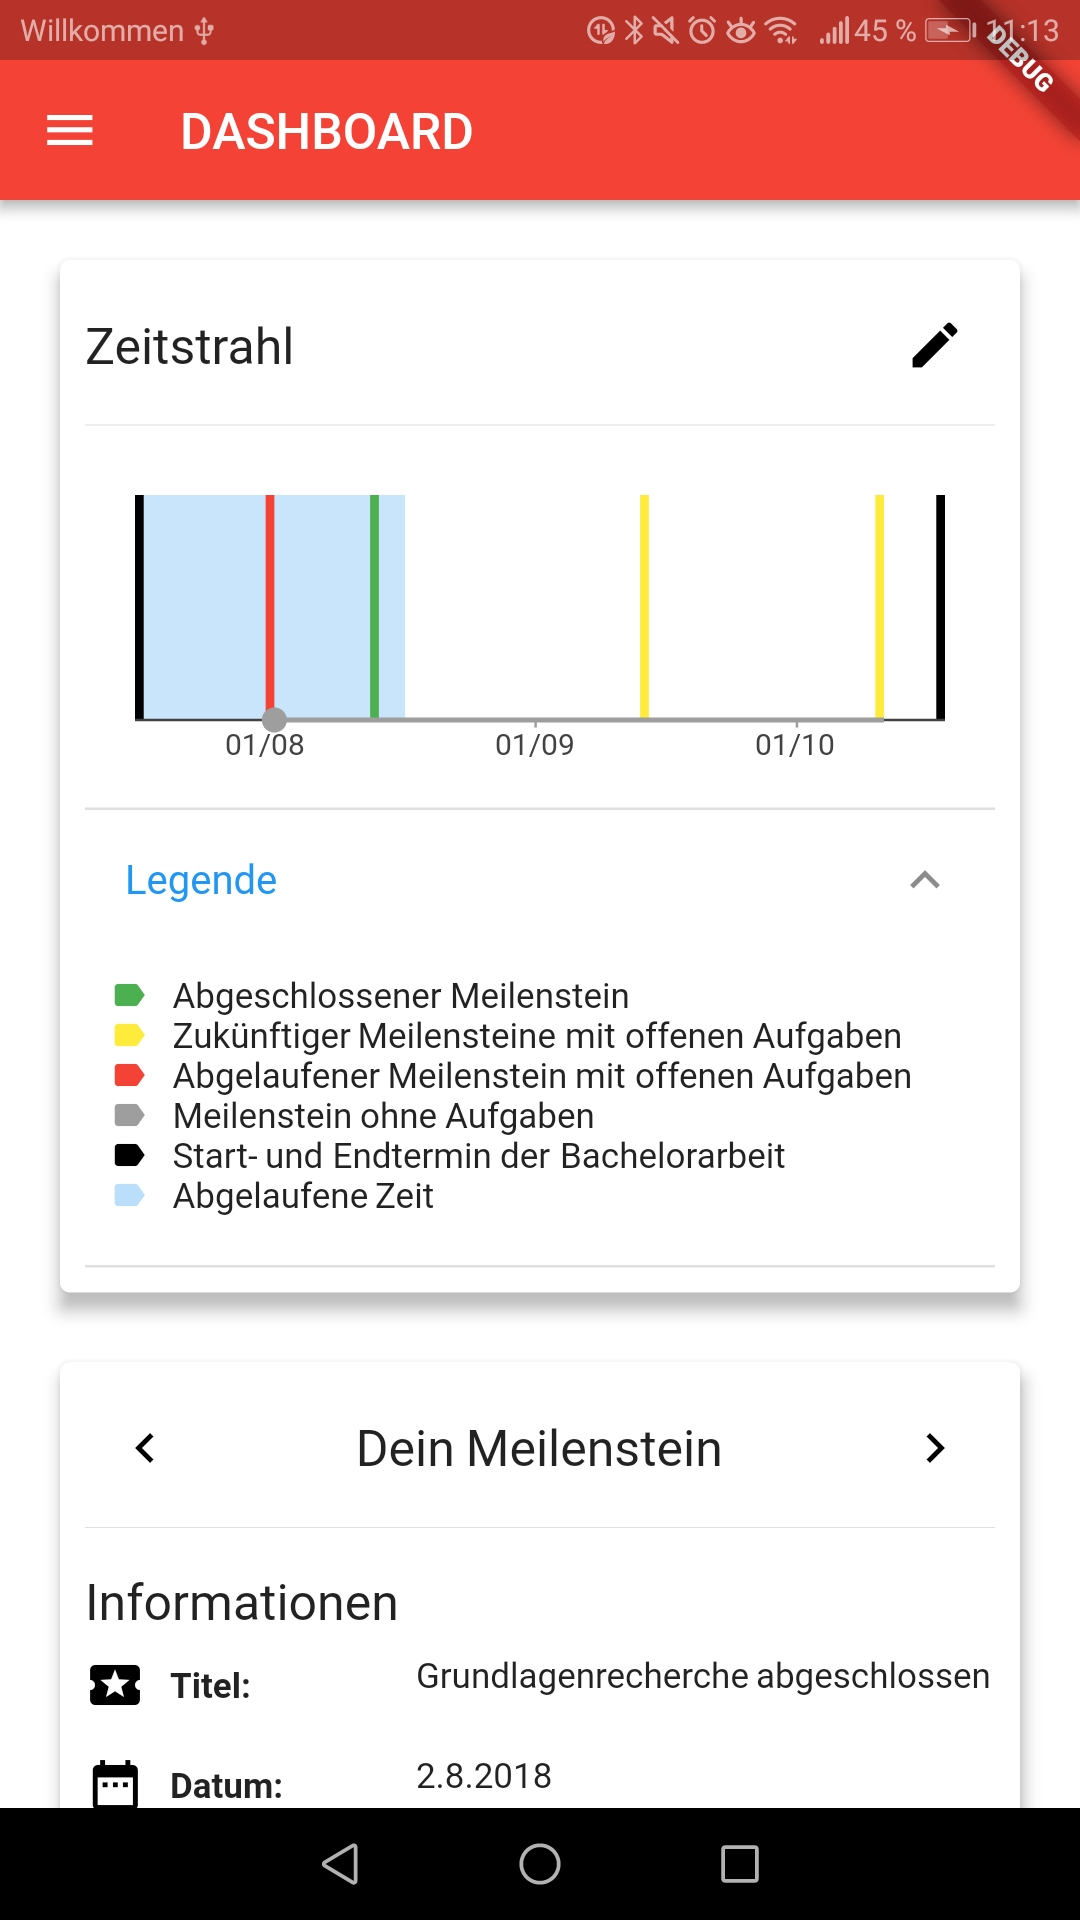
\includegraphics[width=0.4\textwidth,keepaspectratio]{Bilder/Prototyp/app_screenshots/DashboardScreenshot.jpg}
	\caption{Benutzeroberfläche Dashboard}
	\label{img:dashboard}
\end{figure}

\par Der auf Abbildung \ref{img:dashboard} Auschnitt zeigt einen Zeitstrahl als primäres Fotschrittsverfolgungs-Tool. Dieser Zeitstrahl zeigt die von dem Nutzer erstellte Meilensteine sowie deren zugehörigen Status in Form einer spezifischen Farbvisualisation. Die hierbei übermittelten Informationen ermöglichen dem Benutzer einen Überblick über abgelaufene (rot), aktive (gelb) erfüllte (grün) und statuslose (grau) Meilensteine. 
\par Des weiteren wird dem Benutzer durch einen blau visualisierten bereich die bereits abgelaufene Zeit verdeutlicht, welche zwischen Start und Endpunkt der Bearbeitungszeit auf einfache Weise eine bessere Einschätzung von Fortschritt- und Zeitmanagement ermöglichen soll.

\par \bigskip Auf dem Dashboard befindet sich auch ein Abschnitt, welcher den aktuellen ausgewählten Meilenstein anzeigt. Dieser kann durch Interaktion mit dem Zeitstrahl oder mit den dafür vorgesehenen Pfeilen ausgewählt werden, so dass jederzeit Unteraufgaben abgehakt oder hinzugefüht werden können.

\newpage
\par \bigskip Es folgt eine stichpunktartige Auflistung und Beschreibung weiterer möglicher Ideen zu Inhalten des Dashboards, welche bei der Planung der Software entwickelt wurden und durch einen frühen Oberflächenprototyp in die Anforderungsanalyse eingebunden wurde (siehe Anhang TODO):
\begin{itemize}
\item \textbf{Dynamische Anzeige des Fortschritts}
\par Der bisher geleistete Gesamtfortschritt wird verdeutlicht, indem zu sehen ist, wie viele Meilensteine in Relation zu den Gesamtmeilensteinen bisher abschlossen wurden. Weiterhin wird der bisher geleistete Wochenfortschritt verdeutlicht, indem zu sehen ist, wie viele Aufgabenpakete in der Phase bis zum nächsten Meilenstein, in Relation zu den vorher definierten gesamten Arbeitspaketen, schon erfüllt wurden.
\item \textbf{Anzeige der noch offenen Herausforderungen}
\par Es wird angezeigt, wie viele Herausforderungen der jeweiligen Kategorien abgeschlossen wurden, in Relation zu deren Gesamtanzahl.
\item \textbf{Dynamische Anzeige der letzten erreichten Achievements}
\par Die Anzeige zeigt die letzten erreichten Achievements an. Zugehörig sind in diesem Fall die Darstellung des Typs des Achievements in Form der jeweiligen Färbung und des Titels der Herausforderung. Das zuletzt erreichte Achievement wird hierbei durch Größe der Darstellung und Beschreibung hervorgehoben.
\item \textbf{Dynamische Anzeige von allgemeinen Tipps}
\par Die Anzeige zeigt zufällig ausgewählte allgemeine Tipps zur Bearbeitung der Bachelorarbeit, die im Laufe der Zeit wechseln. 
\end{itemize}

\newpage
\subsection{Übersicht der Produktfunktionen}
\par Die unterschiedlichen Abschnitte der Software stehen unterschiedlich stark in Verbindung mit den verschiedenen definierten Produktanforderungen. Um eine Übersicht über die groben Zusammenhänge zu ermöglichen, folgt eine zusammenfassende Tabelle (Siehe Tabelle \ref{tab:abdeckungProduktfunktionen}).
\bigskip

\begin{tabularx}{\textwidth}{l|X|c|c|c|c|c|c}
\toprule
\textbf{Bezeichnung} 
& \textbf{Beschreibung} 
& \textbf{A1} 
& \textbf{A2} 
& \textbf{A3} 
& \textbf{A4} 
& \textbf{A5} 
& \textbf{A6}
\\ \midrule
	
\textbf{\ref{anf:meilensteinVerwalten}}
&  (Verwaltung von Meilensteinen) 
& \ding{108} 
&  
&  
&  
& \ding{108} 
&  
\\ \midrule
	
\textbf{\ref{anf:arbeitspaketVerwalten}}
& (Verwaltung von Aufgaben) 
& \ding{108} 
&  
&  
&  
& \ding{108} 
&  
\\ \midrule
	
\textbf{\ref{anf:erinnerungenBenachrichtigungen}}
& (Erinnerung an Meilensteine) 
& \ding{108} 
&  
&  
&  
& \ding{108} 
&  
\\ \midrule
	
\textbf{\ref{anf:infRahmenbedingungenFormalien}}
& (Hinweise zu Rahmenbedingungen und Formalien) 
&  
& \ding{108} 
&  
&  
&  
&  
\\ \midrule
	
\textbf{\ref{anf:infAufbauStruktur}}
& (Hinweise zu Aufbau und Struktur) 
&  
& \ding{108} 
&  
&  
&  
&  
\\ \midrule
	
\textbf{\ref{anf:infDurchfuerungBachelorarbeit}}
& (Hinweise zu Durchführung) 
&  
& \ding{108} 
&  
&  
&  
&  
\\ \midrule
	
\textbf{\ref{anf:infMethodenTechniken}}
& (Übersicht von Methoden und Techniken) 
&  
& \ding{108} 
&  
& 
&  
&  
\\ \midrule
	
\textbf{\ref{anf:anpassungZielgruppen}}
& (Anpassbarkeit an Zielgruppe) 
&  
& \ding{108} 
&  
&  
&  
&  
\\ \midrule
	
\textbf{\ref{anf:anpassungSoftwareextern}}
& (Software-externe Anpassung) 
&  
& \ding{108} 
&  
&  
&  
&  \\ \midrule
	
\textbf{\ref{anf:spielDesignElementeBenutzerklassen}}
& (Benutzerklassen-orientierte Spiel-Design-Elemente) 
&  
&  
& \ding{108} 
& \ding{108} 
& \ding{109} 
&  
\\ \midrule
	
\textbf{\ref{anf:spielDesignElementeOrientiertungAnBachelorarabeit}}
& (Spiel-Design-Elemente sinnvoll an Bachelorarbeit orientieren) 
&  
&  
& \ding{108} 
& \ding{108} 
&  
&  
\\ \midrule
	
\textbf{\ref{anf:mehrsprachig}}
& (Mehrsprachigkeit) 
&  
&  
&  
&  
&  
& \ding{109} 
\\ \midrule
	
\textbf{\ref{anf:persoenlicheThemenvorschlaege}}
& (Bachelorarbeitsthemen über Applikation ausschreiben)
&   
&   
&   
&  
&  
& \ding{109} 
\\ \midrule
\bottomrule
\end{tabularx}
\begin{tablenotes}
\item  A1 - Meilensteinverwaltung
\item  A2 - Bachelorarbeit Guide
\item  A3 - Herausforderungen
\item  A4 - Achievements
\item  A5 - Dashboard 
\item  A6 - Sonstige Softwareinhalte
\item \ding{108} - Teil der Applikation
\item \ding{109} - Als Erweiterung vorgesehen
\end{tablenotes} 
\captionof{table}{Abdeckung der Produktfunktionen}
\label{tab:abdeckungProduktfunktionen}

\newpage
\subsection{Umgang mit Risiken}
\par Im folgenden Verlauf wird der Umgang mit den, in Kapitel \ref{sub:risikouebersicht} dargestellten, Risiken diskutiert und beschrieben.
\par \medskip Da sich die Herausforderungen an dem Ablauf einer Bachelorarbeit orientieren und den Studierenden somit vor typische Aufgaben stellt, kam es im Verlauf der Interviews zu den Befürchtungen \ref{risk:realerZustand}, dass die Applikation nicht den realen Zustand der Bachelorarbeit kennt und somit der Studierende durch das Erfüllen von Herausforderungen ein Gefühl von Erfolg hat, obwohl diese Herausforderungen nicht den geforderten Qualitäten entsprechen und der Studierende dies durch das positive Feedback nicht merkt.
\par Um diesem Risiko entgegenzuwirken sollen die erstellten Herausforderungen möglichst auffordernder Natur sein (Beispiel: Beginne deine Einleitung). Bei Einsatz von Herausforderungen, welche auf inhaltliche Aspekte abzielen, sollen Checklisten zum Abschließen der Herausforderungen genutzt werden, um den Fokus auf eine allgemeingültige Vorgehensweise zu reduzieren, für deren Erfüllung die Studierenden jedoch selbst verantwortlich sind. Auch hier wird eine klare Kommunikation durch die Applikation als zwingend erforderlich angesehen.

\par \medskip Die Befürchtung \ref{risk:keinLerneffekt}, dass die Applikation den Studierenden so viel Arbeit abnimmt, dass sie zu wenig eigenständige Erfahrung sammeln und somit der Lerneffekt zu gering ist, wird berücksichtigt, indem die Applikation einen eher informierenden Charakter aufweist, und keine Funktionalität bezüglich dem Liefern von Ergebnissen vorsieht.

\par \medskip Die Gefahren der Risiken \ref{risk:inhaltUnumstoesslich} und \ref{risk:erstazBetreuer}, die sich damit befassen, dass die Applikation fälschlicherweise als Ersatz eines Betreuers wahrgenommen oder der Inhalt der Applikation als unumstößlich angesehen werden könnte, soll durch eine klare Kommunikation mit den Anwendern reduziert werden. Es werden als Maßnahmen einerseits immer die Quellen der Informationen angegeben und weiterhin eine allgemein sichtbare Erklärung zur Anwendung oder Fehlanwendung der Applikation deutlich kommuniziert.

\par \medskip  Das identifizierte Risiko \ref{risk:ueberplanung}, welches die Befürchtung einer Überplanung der Studierenden beinhaltet, was die Auswirkung haben kann, dass die Studierenden von der eigentlichen Arbeit abgehalten werden, wird als nicht ausschlaggebend betrachtet.
Studierende, die zur Überplanung neigen, würden dies auch ohne Applikation tun. 
\par Wichtiger wird in dieser Hinsicht die Freiheit der einzelnen Planungs-Bedürfnisse durch die individuelle Arbeitsweise der Studierenden angesehen, weshalb keine weiteren Maßnahmen zur Reduzierung der Planungsfreiheit getroffen werden. Weiterhin steht die Intensität der Planung nicht in der Verantwortung der Applikation, sondern in der Verantwortung des Benutzers. 

\par \medskip Das Risiko \ref{risk:gamificationEffekt}, das sich mit dem Nichtwirken der Gamification-Motivation befasst, wird als nicht weitreichend betrachtet, da die Gamification-Inhalte zwar Bestandteil der Applikation, jedoch nicht zwangsweise notwendig zur Benutzung der Applikation sind. Die Spiel-Design-Elemente sollen nicht das Interesse an einem bestimmten Thema steigern, sondern dienen im Kontext der Bachelorarbeit einer wegweisenden Natur, welche motivierende Einflüsse auf die Bearbeitenden hervorrufen können, jedoch nicht müssen, um ihren Nutzen zu erfüllen. 

\newpage
\section{Beschreibung der Gamification-Elemente} \label{sec:gamificationelemente}
\par Im folgenden Kapitel werden die Gamification-Elemente, die in der Applikation zum Einsatz kommen, näher beschrieben. Dabei wird vor allem auf die identifizierten Kategorien der Achievements eingegangen, welche den Kern der gewählten Motivationsstrategie bilden. Darüber hinaus wird auch beschrieben, in welcher Form die gewählte Motivationsstrategie in der Realität, in Bezug auf den Fortschritt bei der Bearbeitung der Bachelorarbeit, funktioniert.

\subsection{Achievements} \label{sub:konzeptGamificationAchievements}
\par Die Achievements verfolgen im Rahmen der Applikation die Aufgabe, motivierende Inhalte vor allem für die identifizierten Benutzergruppen der \textbf{Achiever} und \textbf{Explorer} (siehe \ref{sub:nutzergruppenBartle}) zu bieten. Dies soll erreicht werden, indem die Achievements dem Benutzer als Belohnung für eine abgeschlossene Herausforderung als Sammelstück hinzugefügt werden.
\par \medskip Im Rahmen der gewählten Motivationsstrategie werden verschiedenen Arten von Achievements in die Applikation integriert. Dies passiert unter anderem mit dem Ziel, eine an den Ablauf einer Bachelorarbeit gekoppelte Abstufung von Fortschritt und Erfolgen zu ermöglichen. 
\par Weiterhin werden auch die sogenannten \textit{App-Achievements} Einzug in die Applikation erhalten. Diese sollen weitestgehend die Bedürfnisse der Benutzergruppe \textbf{Explorer} ansprechen und im Gegensatz zu den anderen Achievements nicht an einer konkreten Herausforderung gekoppelt sein, sondern im Laufe der Nutzung der Applikation durch \textit{versteckte Aufgaben} freigeschaltet und offen gelegt werden können.

\par \medskip Um den Achievements, über das Sammeln und die Vervollständigung hinaus, eine Wertigkeit zu geben, werden diese durch verschieden visualisierte Medaillen dargestellt. 

\bigskip
\begin{figure}[H]
\centering

	{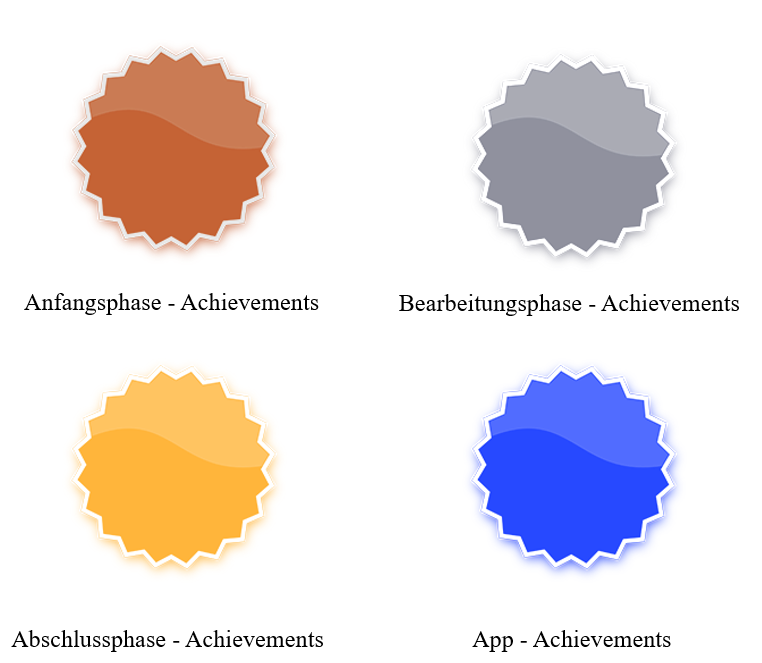
\includegraphics[width=0.65\textwidth]{Bilder/AchievementsVisualisierung.png}}

	\caption{Visualisierung der Achievements}
	\label{img:achievements}
\end{figure}

\par \bigskip Diese Achievements basieren auf einem Bild aus der gemeinfreien Bilderdatenbank Pixabay (vgl. \citep{PixabayAchievement}) und wurden mit einer Bilderbearbeitungssoftware für die eigenen Zwecke bearbeitet.

\par \bigskip Es folgt eine Übersicht und Beschreibung der verschiedenen Achievement-Typen:
\begin{itemize}
\item \textbf{Anfangsphase-Achievements} (Bronze)
\par Beinhaltete Achievements, die an die Herausforderungen gekoppelt sind, die nach Beginn der Bachelorarbeit erfolgen, sich aber noch nicht mit den einzelnen inhaltlichen Schritten der Bachelorarbeit auseinandersetzen.
\item \textbf{Bearbeitungsphase-Achievements} (Silber)
\par Beinhaltete Achievements, welche an die Herausforderungen gekoppelt sind, die nach Beginn der Bachelorarbeit erfolgen und sich mit der eigentlichen Bearbeitung der Bachelorarbeit auseinandersetzen.
\item \textbf{Abschlussphase-Achievements} (Gold)
\par Beinhaltete Achievements, welche an die Herausforderungen gekoppelt sind, die sich hauptsächlich mit der Abschlussphase einer Bachelorarbeit beschäftigen.
\item \textbf{App-Achievements} (Blau)
\par Beinhaltete Achievements, welche an keinen offensichtlichen Herausforderungen gekoppelt sind, sondern nur durch Benutzung der Applikation erhalten werden können. Die hierbei von den klassischen Abstufung der Wertigkeit (Bronze, Silber, Gold) gewählte Farbe (Blau) soll die semantische Differenz zwischen den Herausforderungen und den, durch die Benutzung der App ausgelösten, Achievements verdeutlichen. 
\end{itemize} 

\par \bigskip Der Inhalt wird durch unterschiedliche, den Achievements entsprechenden, Texten dargestellt. Hierbei geht es darum, die mit den Herausforderungen gekoppelten Achievements durch das Verfassen passender Texte eine Ausstrahlung zu verleihen, welche dem Benutzer, als Reaktion auf die Erfüllung eines Achievements, als Titel angezeigt wird. Der Inhalt der Texte ist nicht festgelegt, sollte jedoch so gewählt werden, dass eine positive oder ironische Stimmung gegenüber dem Benutzer vermittelt wird.
\par \bigskip \textit{Hinweis: Eine für den Protypen gewählte Übersicht der Achievements ist im Anhang zu finden (siehe Angang TODO).}

\newpage
\chapter{Architektur und  prototypische Implementierungsdetails} \label{chap:architektur}
\par Das Ziel dieses Kapitels ist es, das Verständnis für die architekturspezifischen Zusammenhänge sowie die jeweiligen softwaretechnischen Abläufe zu vermitteln. 
\par Auf dieser Basis werden die einzelnen Architektur-Komponenten, deren Beziehungen zueinander sowie die Funktionsweise des Gesamtsystems im folgenden Verlauf erläutert und in Kapitel Die detaillierte Beschreibung der einzelnen Komponenten folgt in Kapitel \ref{sec:komponentenDetails} an geeigneter Stelle durch beispielhafte Abläufen von Nutzeraktionen beschrieben.

\section{Architekturübersicht}
\par Aufgrund der Vorzüge einer konsequenten zentralen Verwaltung des Zustands der Applikation, welche in diesem Rahmen auch mit einer komfortablen Wartbarkeit und den strikt getrennten und auf diese Weise auch eindeutig nachverfolgbaren Datenflüssen und Operationen einhergeht, wurde eine Architektur konstruiert, die sich an dem Redux-Architekturmuster orientiert. 
\par Die folgende Abbildung \ref{img:architectureOverview} soll in vereinfachter Form verdeutlichen, wie die verschiedenen Komponenten der gewählten Architektur hinsichtlich des Aufbaus und des Datenflusses zueinander in Beziehung stehen. 

\begin{figure}[H]
	\centering
	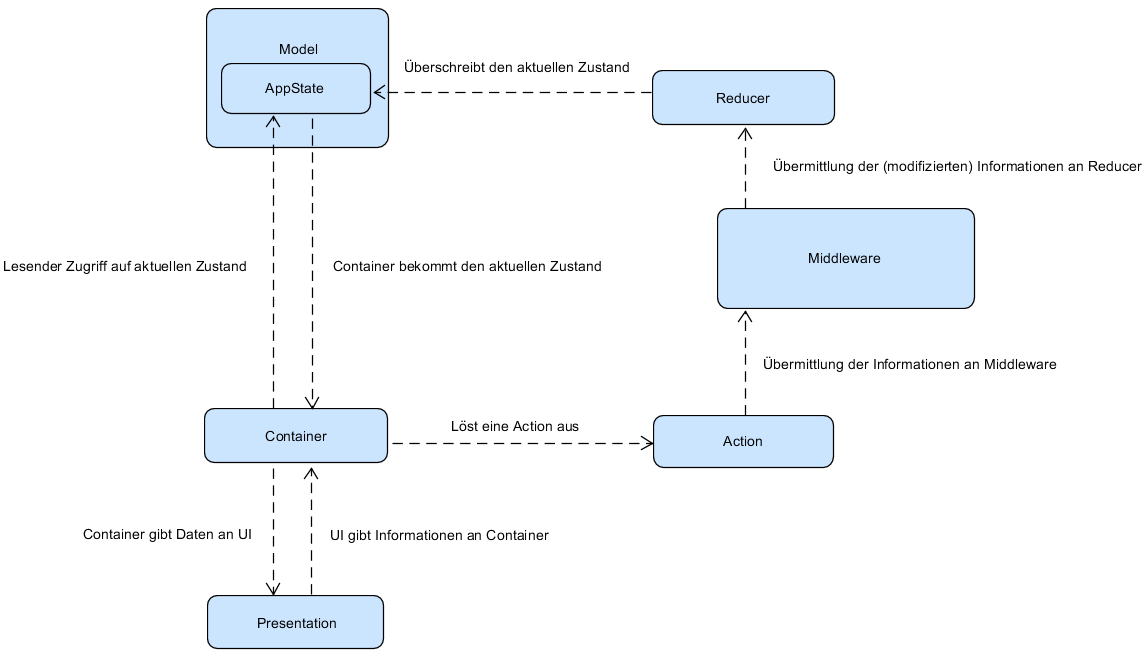
\includegraphics[width=0.95\textwidth,keepaspectratio]{Bilder/ArchitectureOverview.png}
	\caption{Architekturübersicht}
	\label{img:architectureOverview}
\end{figure}

\par \bigskip \textbf{Model}
\par Die Model-Komponenten stellen den aktuellen internen Zustand des Systems dar und enthalten somit in erster Linie die hierfür verwendeten Objekt-Klassen.
\par Die für die gewählte Architektur durch ihre Wichtigkeit hervorzuhebende Klasse AppState, ist die zentrale Verwaltungsklasse für den gespeicherten Status der Applikation und trägt alle relevanten Informationen in sich, die den aktuellen Zustand des Systems abbilden. Die Klasse AppState selbst dient also lediglich als zentrales Element zur Datenhaltung in der gewählten Architektur.

\par \bigskip \textbf{Presentation}
\par Die Presentation-Komponenten sind alleinig für die Visualisierung der gegebenen Informationen sowie für die Entgegennahme der Benutzereingaben zuständig.

\par \bigskip \textbf{Container}
\par Die Container-Komponenten lesen den aktuellen Zustand der Applikation aus dem AppState ein und bereiten diesen vor der Übergabe an die Presentation-Komponenten vor. Weiterhin lösen die Container-Komponenten die Actions aus, welche auf den von dem Benutzer getätigten Interaktionen basieren.

\par \bigskip \textbf{Action}
\par Eine Action-Komponente beinhaltet Informationen über die jeweilige auszuführende Operation und dient somit als Identifikationsmittel und Informationspaket, die von der Middleware und/oder den Reducer-Komponenten aufgegriffen und verarbeitet werden.

\par \bigskip \textbf{Middleware}
\par Die Middleware verarbeitet und/oder manipuliert die, in den Actions übermittelten, Informationen, bevor diese zu den Reducer-Komponenten gelangen. Weiterhin können auch in der Middleware selbst Actions ausgelöst werden, wie im späteren Verlauf in Kapitel \ref{sec:middleware} nachzuvollziehen ist. 

\par \bigskip \textbf{Reducer}
\par Die Reducer-Komponenten nehmen die eigentliche Änderung am Zustand vor, indem sie einen völlig neuen Zustand generieren und den vorherigen Zustand überschreiben. Durch die, über die Actions erhaltene, Informationen weiß die Reducer-Komponente, welche Aktion der Benutzer ausgeführt hat und folglich auch, welche Information sich an dem aktuell existierenden Zustand der Applikation ändern soll. In diesen Komponenten wird also der aktuelle Zustand in einen neuen Zustand transformiert.

\newpage
\section{Detaillierte Beschreibung der Model Komponenten}
\label{sec:komponentenDetails}
\par \bigskip Die nun folgenden Unterkapitel beschreiben die Klassen, die Teil der Model Komponente sind und teilweise wichtige Datenfelder und Operationen zur Verwaltung des Redux-Stores enthalten.

\par \bigskip \textit{Hinweis: Alle verwendeten Klassen deren Objekt-Instanzen in dem Redux-Store liegen, sind mit dem Schlüsselwort \texttt{@immutable} versehen und können zur Laufzeit nicht verändert werden. Dies ist hinsichtlich der Redux-Architektur vorgesehen, da der Redux-Store und dessen Inhalt nicht verändert, sondern überschrieben wird. Weiterhin liegen die Attribute innerhalb der Objekt-Klassen im Rahmen des flach ausgerichteten Key-Value-Stores des AppStates im Allgemeinen nicht als Objektreferenzen, sondern als IDs in textueller Form vor.}

\subsection{AppState-Klasse}
\par Die Klasse AppState stellt den aktuellen Status der Applikation dar und trägt somit eine Vielzahl an Informationen in sich. Diese Informationen werden im Rahmen der an Redux orientierten Architektur durch das Einsetzen von Key-Value Stores strukturiert und verwaltet. 

\par \medskip Jede für den Zustand der Applikation relevante Information ist auf diese Weise an einer zentralen Stelle im System gespeichert (siehe Listing \ref{lst:appstateFields}). Durch einen lesenden Zugriff können die Oberflächenkomponenten alle benötigten aktuellen Informationen ermitteln und abbilden. Weiterhin kann der Status der Applikation durch das Ausführen von Aktionen des Benutzers, was das Auslösen der sogenannten Actions mit sich trägt, verändert werden.
  
  \bigskip
 \begin{lstlisting}[caption={Datenfelder der AppState-Klasse},captionpos=b, label=lst:appstateFields]
class AppState{

  final Map<String, Milestone> currentMilestones;
  final Map<String, Map<String, Achievement>> achievedAchievements;
  final Map<String, Property> properties;
  final Map<String, Challenge> challenges;
  final Map<String, Content> informationToolContent; 
 
  final Milestone selectedMilestone;
  final DateTime begin;
  final DateTime end;

	...
  }
\end{lstlisting}
\bigskip



\par \bigskip \textbf{Aktueller Zustand der Meilensteine}
\par Die aktuellen Meilensteine werden durch das Datenfeld currentMilestones abgebildet. Diese Datenstruktur enthält alle vom Benutzer angelegten Meilensteine und deren jeweilige Unteraufgaben und wird als SplayTreeMap initialisiert. Die selbst-sortierende Eigenschaft dieser Datenstruktur bietet einige Vorteile im Rahmen der Handhabung von Meilensteinen in der Implementierung, da deren einzigartige IDs auf dem angegebenen Meilensteindatum basieren.

\par \bigskip \textbf{Aktueller Zustand der Achievements}
\par Die von dem Benutzer der Applikation zu erreichenden Achievements werden im Datenfeld achievements gespeichert. Dieses Datenfeld weißt einige Besonderheiten vor, auf die ich im Folgenden hinweisen möchte:
\par \medskip  \textit{Hinweis: Es handelt sich bei dieser Datenstruktur im Detail um eine HashMap, welche weitere HashMaps beinhaltet.}
\par \medskip Diese HashMap wird mit genau vier verschiedenen konstanten Einträgen initialisiert.
\begin{itemize}
\item \textbf{ALL\char`_ACHIEVEMENTS}
\par Enthält alle vorhandenen Achievements.
\item \textbf{ACHIEVED}
\par Enthält alle Achievements, die von dem Benutzer gesammelt wurden.
\item \textbf{RECOGNIZED}
\par Enthält alle gesammelten Achievements, die von dem Benutzer betrachtet wurden.
\item \textbf{NOT\char`_RECOGNIZED}
\par Enthält alle gesammelten Achievements, die von dem Benutzer noch nicht betrachtet wurden.
\end{itemize}

\par Diese Unterscheidung ist durch die Idee begründet, die unterschiedlichen Zustände der Achievements bei der Handhabung der Benutzerinteraktion zu unterschiedlicher Zeit zu berücksichtigen. Beispielsweise sollen neu erworbene Achievements, welche vom Benutzer noch nicht eingesehen worden sind, bis zu dem Moment, in dem sie betrachtet wurden, gesondert behandelt werden.

\par \bigskip \textbf{Aktueller Zustand der Properties}
\par Die zu verwaltenden Eigenschaften zur Erfüllung der Achievements werden in dem Datenfeld properties gespeichert. Dies bietet den Vorteil, dass die Properties, welche von unterschiedlichen Achievements geteilt werden können, an einer zentralen Stelle im State verwaltet werden können.

\par \bigskip \textbf{Aktueller Zustand der Herausforderungen}
\par Die für den Benutzer zu erledigenden Herausforderungen werden in dem Datenfeld challenges verwaltet.
Über die bereits genannten Verwaltungsstrukturen hinaus beinhaltet die Klasse weiterhin folgende einzelne Informationen:

\par \bigskip \textbf{Aktueller Zustand des Bachelorarbeit-Guide Inhaltes}
\par Der aus einem Git Repository ausgelesene und durch Content-Objekte strukturierte Inhalt des Bachelorarbeit-Guides wird in dem Datenfeld informationToolContent verwaltet.

\par \bigskip \textbf{Weitere Datenfelder}
\par Der aktuell, im Rahmen der Bedienung der Applikation von dem Nutzer ausgewählte, Meilenstein wird im Datenfeld \texttt{selectedMilestone} gespeichert. 
\par \medskip Die beiden Felder \texttt{begin} und \texttt{end}, bezeichnen den durch den Benutzer angegebenen Bearbeitungszeitraum der Bachelorarbeit.

\newpage
\subsection{Milestone-Klasse}
\par Ein Meilenstein besitzt folgende Attribute und Methoden:

\begin{itemize}

\item[] \texttt{\textbf{String id}}
\par Jeder Meilenstein besitzt eine ID, die immer auf dem jeweils festgelegten Datum des Meilensteins basiert.

\item[] \texttt{\textbf{String title}}
\par Der eigentliche Titel beschreibt den, von dem Benutzer gegebenen, Namen des Meilensteins und dient als Identifikations- und Anzeigemittel für den Benutzer.

\item[] \texttt{\textbf{String description}}
\par In dem Datenfeld description befindet sich die von dem Benutzer eingetragene Beschreibung des Meilensteins.

\item[] \texttt{\textbf{DateTime date}}
\par Jeder Meilenstein muss ein Ablaufdatum enthalten, welches den Tag darstellt, an dem der Meilenstein eingetragen ist.

\item[] \texttt{\textbf{Map<String, Task> tasks}}
\par Meilensteine besitzen, von dem Benutzer hinzugefügte, Unteraufgaben, die in dem Datenfeld tasks liegen.

\item[] \texttt{\textbf{Map<String, Task> getCompletedTasks(), getNotCompletedTasks()}}
\par Durch die Methoden getCompletedTasks() und getNotCompletedTasks() ist die Möglichkeit gegeben, abgeschlossene und noch offene Unteraufgaben der Meilensteine herauszufiltern.

\item[] \texttt{\textbf{MilestoneState getMilestoneState()}}
\par Durch die Methode getMilestoneState() bietet sich die Möglichkeit, den aktuellen Status des Meilensteins zu bestimmen, welcher auf abgeschlossene Unteraufgaben, noch offene Unteraufgaben sowie der Relation zwischen dem aktuellen Zeitpunkt und dem definierten Ablaufzeitpunkt basiert. Für diesen Zweck wird weiterhin die Enumeration MilestoneState verwendet, die die vier Zustände Empty, AllTasksCompleted, SomeTasksNotCompleted und outOfDateAndSomeTasksNotCompleted darstellt.
\end{itemize}

\newpage

\subsection{Task-Klasse}
\par Ein Task besitzt folgende Attribute:

\begin{itemize}
\item[] \texttt{\textbf{String id}}
\par Jeder Task besitzt eine ID als Identifikationsmöglichkeit.

\item[] \texttt{\textbf{String title}}
\par Der Titel eines Tasks stellt die, von dem Nutzer erstellte, inhaltlich zu lösende Aufgabe dar.

\item[] \texttt{\textbf{TaskState taskState}}
\par Ein Task kann die Zustände \texttt{Completed} und \texttt{NotCompleted} annehmen, welche durch eine Enumeration dargestellt werden. Eine Enumeration wurde einem booleschen Wert vorgezogen, da weitere Zustände, wie zum Beispiel das Favorisieren von Unteraufgaben, bei Bedarf hinzugefügt werden könnten.
\end{itemize}

\subsection{Challenge-Klasse}
Die von dem Benutzer zu absolvierenden Herausforderungen enthalten folgende Attribute:

\begin{itemize}
\item[] \texttt{\textbf{String title}}
\par Jede Herausforderung besitzt einen Titel, welche den Inhalt der zu absolvierenden Aufgabe darstellt. Dies ist also der Inhalt, welcher der Benutzer in der Applikation angezeigt bekommt.
\item[] \texttt{\textbf{ChallengeType type}}
\par Der Typ einer Challenge lässt sich durch eine definierte Enumeration ausdrücken. Vorgesehen ist dies, um den jeweiligen Herausforderungen einen Kontext zu verleihen. Als Beispiel kann hier eine Aufteilung in verschiedene Phasen der Bachelorarbeit erfolgen.
\item[] \texttt{\textbf{bool completed}}
\par Ob eine Herausforderung abgeschlossen wurde oder noch offen ist, wird über das Feld \texttt{completed} angegeben.
\end{itemize}

\subsection{Achievement-Klasse}
\par Ein Achievement besitzt folgende Attribute:

\begin{itemize}
\item[] \texttt{\textbf{String title}}
\par Der Titel des Achievements ist der Teil, der dem Nutzer als Identifikationsmittel des jeweiligen Achievements angezeigt wird.  

\item[] \texttt{\textbf{bool completed}}
\par Die Information, ob ein Achievement erreicht wurde, wird durch den Wert des Attributs completed dargestellt.

\item[] \texttt{\textbf{List<String> properties}}
\par Weiterhin beinhaltet ein Achievement bestimmte Eigenschaften, die erfüllt werden müssen, damit das Achievement als erreicht bezeichnet werden kann. Ein Achievement wird also nur erreicht, wenn alle seine Properties als erfüllt gelten.  

\item[] \texttt{\textbf{AchievementType type}}
\par Der Typ, welcher durch eine Enumeration verdeutlicht wird, stellt die Art des Achievements dar.
\end{itemize}

\par \textit{Hinweis: Bei der nicht ganz einfachen Implementierung von Achievements wurde sich nach ausgiebiger Recherche an einem im Internet geteilten Beitrag (vgl. \citep{AchievementsImplementation}) orientiert und die dort beschriebene Umsetzung für die eigene Redux-basierte Variante adaptiert.}

\subsection{Property-Klasse}
\label{sub:propertyclass}
\par \medskip Die Klasse Property enthält folgende Attribute und Funktionen:

\begin{itemize}
\item[] \texttt{\textbf{String name}}
\par Der Name einer Property-Instanz stellt die Bezeichnung dar, welche dem Nutzer als Identifikationsmöglichkeit dient und im Rahmen der Applikation als Instruktion angezeigt werden kann, weshalb diese Bezeichnung wohlüberlegt gewählt werden sollte. 

\item[] \texttt{\textbf{int initialValue}}
\par Der Initialwert beschreibt, wie der Name bereits impliziert, den Startwert, der bei Initialisieren des Objektes angenommen wird.

\item[] \texttt{\textbf{int currentValue}}
\par Ein aktueller Wert stellt den aktuellen Fortschritt der jeweiligen Eigenschaft, welche es zu erfüllen gilt, dar. 

\item[] \texttt{\textbf{int activationValue}}
\par Das Datenfeld activationValue stellt den Zielwert dar, den es zu erfüllen gilt.

\item[] \texttt{\textbf{String activiationRule}}
\par Die genannten Felder \texttt{initialValue}, \texttt{currentValue} und \texttt{activationValue} werden durch eine definierte Regel in Beziehung zueinander gesetzt. Diese Regel kann verschieden ausgeprägt sein, um dem Ersteller von Achievements sowie deren Kriterien zur Erfüllung eine gewisse Freiheit zu ermöglichen. Im Rahmen des Projektes wurden drei verschiedene Regeln in Form von konstanten Variablen des Datentyps String aufgestellt, welche die Regeln \grqq <\grqq, \grqq >\grqq und \grqq ==\grqq enthalten. 

\item[] \texttt{\textbf{bool isActive()}}
\par Diese Regeln werden als Werkzeug benutzt, um die Semantik der zu erfüllenden Eigenschaften auf die logische Ebene zu übertragen.
Beispielsweise kann somit in der Methode isActive() überprüft werden, ob der Benutzer bereits drei Meilensteine erstellt hat, also die jeweilige Eigenschaft erfüllt wurde.

\end{itemize}

\subsection{Content-Klasse}
\par Eine Objektinstanz der Content-Klasse stellt den Inhalt der \grqq Guide\grqq -Funktion dar und enthält folgende Attribute:
\begin{itemize}

\item[] \texttt{\textbf{String id}}
\par Die ID eines Content-Objekts dient als Zuweisungsmittel von weiteren Content-Objekten als Unterabschnitten. Die verwendeten IDs werden in der ausgelesenen JSON-Datei, welche in dem Git-Repository liegt, zugewiesen

\item[] \texttt{\textbf{String title, description}}
\par Der Titel des Content-Objekts ist gleichzusetzen mit einer Überschrift für den jeweiligen Inhalt, der durch die Beschreibung ausgedrückt wird.

\item[] \texttt{\textbf{List<String> subsections}}
\par Das Datenfeld subsections enthält Referenzen durch in textueller Form zugewiesenen IDs weiterer Content-Objekte, welche in Beziehung mit dem jeweils übergeordneten Content-Objekts als Unterabschnitte zu bezeichnen sind.

\item[] \texttt{\textbf{String type}}
\par Der Typ enthält Informationen darüber, welche Art von Darstellung innerhalb des \grqq Guide\grqq -Tools für die Benutzeroberfläche verwendet werden soll. Das bietet den Vorteil, dass bei dem Erstellen der JSON-Datei für den Inhalt dieser Funktion keine Kenntnisse über die softwareinterne Lösung vorhanden sein muss, sondern der Ersteller nur vordefinierte Begriffe eintragen muss, die dann softwareintern den jeweiligen Bildschirminhalt generieren.
\end{itemize}

\par \bigskip \textit{Hinweis: Im Rahmen der Prototypentwicklung sind zwei verschiedene Arten (type) der Darstellung von Content-Objekten vorgesehen:}
\begin{itemize}
\item[\textit{1.}] \textit{Die erste Möglichkeit ist das Erzeugen eines Buttons (\grqq ButtonListWidget\grqq), welcher den Titel des Content-Objektes anzeigt und bei Antippen auf eine nächste Seite führt und dort die jeweiligen subsections anzeigt.}
\item[\textit{2.}] \textit{Die zweite Möglichkeit ist das Generieren eines ausklappbaren Elements (\grqq ExtensionPanelWidget\grqq), welches den Titel des Content-Objektes anzeigt und dessen Beschreibung bei Ausklappen sichtbar wird.}
\end{itemize}

\newpage
\subsection{AppContentLoader-Klasse}
\par Die Klasse ContentLoader stellt die Schnittstelle zum gewählten Git-Repository dar und trägt in diesem Umfang die Aufgabe, die in dem Repository-Ordner angelegten JSON-Dateien durch HTTP-Requests  einzulesen und dem System zur weiteren Verarbeitung zur Verfügung zu stellen. Dies wird umgesetzt, indem diese eingelesenen Dateien in lokaler Form auf dem Endgerät gespeichert werden.
\par Die Klasse besitzt lediglich ein Datenfeld (\texttt{String httpRequest}), welches die auszuführende HTTP-Anfrage beinhaltet.

\subsection{JSONAppContentFile-Klasse}
\par Eine Instanz dieser Klasse, die durch eine Objektinstanz der Klasse AppContentLoader erzeugt wird, stellt eine aus dem Repository eingelesene JSON-Datei dar und enthält 
den Namen der im Repository vorliegenden JSON-Datei, welche auch weiterhin als Dateiname in dem lokalen Speicher des Endgeräts verwendet. 
\par Die durch den ContentBuilder ermittelte jeweilige Download-Adresse der verschiedenen im Repository liegenden Dateien, dient zum Herunterladen des jeweiligen Inhaltes der jeweiligen JSON-Datei, was wiederum durch die Methode \texttt{Future<String> getJsonContent()}, im Detail durch ein HTTP-Request umgesetzt wird.

\subsection{InformationToolContentBuilder-Klasse}
\par Die Hilfsklasse InformationToolContentBuilder dient als Werkzeug zur Generierung des Inhaltes der Software-Sektion \grqq Bachelorarbeit Guide\grqq{} der Applikation. Die Content-Objekte werden durch die jeweilige JSON-Datei, welche zuvor aus dem Git-Repository ausgelesen und gespeichert wurde generiert. Jedes Content-Objekt kann mehrere Content-Objekte in Form der jeweiligen IDs referenzieren, welche in diesem Rahmen als subsections bezeichnet werden.

\subsection{Achievement-Notification Funktionen}
\par Für die Implementierung der Notification wurde ein externes Plugin genutzt (siehe \citep{FlutterLocalNotificationPlugin}), da die grundsätzliche Möglichkeit der Handhabung von Notifications durch das Framework Flutter nicht gegeben ist. Durch die Verwendung des Plugins sind jedoch einige zielplattformabhängige Konfigurationen nötig, welche sich unter \citep[Android Integration]{FlutterLocalNotificationPlugin} und \citep[iOS Integration]{FlutterLocalNotificationPlugin} nachvollziehen lassen.
\par \medskip Bei der Umsetzung der Notifications wurde sich an den dort gegebenen Beispielen orientiert, wobei deren Funktionsweisen für die eigene Umsetzung adaptiert wurden.
\par Die Verwendung der Achievement-Notifications wird im Rahmen der prototypischen Implementierung durch spezielle Top-Level-Funktionen gelöst, welche bei Aufrufen die jeweiligen Achievement-Actions auslösen. Die dadurch hervorgerufene Aktualisierung der zu den Achievements zugehörigen Bedingungen findet in der updateProperties Reducer-Funktion statt. Hier werden die Nutzeraktionen an zentraler Stelle im System abgefragt und die Änderungen an den aktuellen, im Zustand gespeicherten, Bedingungen durchgeführt. Somit ist dies die zentral zu erweiternde Stelle im Code, wenn neue Achievements Einzug in das System erhalten.
\par \bigskip Weitere Informationen zum Ablauf und der Funktionsweise von Notifications sind in Kapitel \ref{sec:middleware} zu finden.

\newpage
\section{Actions}
\par Im Rahmen der auf der Anforderungsanalyse basierenden Konzeption der Softwarelösung wurden verschiede Benutzeraktionen identifiziert, welche sich größtenteils in den sogenannten Actions wiederfinden.
Für jede dieser Actions existiert eine eigene Klasse, welche im folgenden Verlauf beispielhaft an einem für alle Actions repräsentativen Fall erläutert wird.

\subsection{Beispielhafte Demonstration einer Meilensteinbearbeitung}
\par Das gewählte Beispiel bezieht sich auf die Nutzeraktion des Änderns eines Meilensteins:

\par Wie in Abbildung \ref{lst:milestoneEditAction} zu sehen ist, enthält die Klasse EditMilestoneAction vier verschiedene Datenfelder. 
Der zu ändernde Meilenstein (\texttt{milestone}) sowie die jeweiligen neuen Werte newTitle, newDate und newDescription, welche die zu dem vorhandenen Meilenstein zugehörigen Werte überschreiben sollen.
\par Es wird deutlich, dass eine solche Klasse außer dem Beinhalten der spezifischen Payload-Daten keine tiefe Funktionalität bieten soll. 
\par Die weitere Verarbeitung der Daten wird im Kapitel \ref{sec:reducer} verdeutlicht.

\bigskip
\begin{lstlisting}[caption={Meilenstein Action Beispiel},captionpos=b, label=lst:milestoneEditAction]
class EditMilestoneAction {
  Milestone milestone;
  String newTitle;
  DateTime newDate;
  String newDescription;

  EditMilestoneAction(this.milestone, this.newTitle, this.newDate, this.newDescription);
}
\end{lstlisting}
\bigskip


\newpage
\section{Reducer}
\label{sec:reducer}
\par Die verschiedenen Reducer-Funktionen tragen die eigentliche Aufgabe der Datenmanipulation und Verwaltung. In diesen Komponenten passieren die entscheidenden Änderungen am aktuellen Zustand der Applikation.

\subsection{App-Reducer}
\par Der App-Reducer ist die Top-Funktion der Reducer, welche nach jeder durchgeführten Action einen neuen Zustand der Applikation generiert. Jedes Datenfeld des aktuellen Zustands wird in diesem Rahmen durch die Delegation an untergeordnete Reducer-Funktionen neu generiert. Dabei wird immer der aktuelle Zustand des Systems sowie die in der Action-Klasse enthaltenen Informationen übergeben.
\par \medskip Im folgenden Verlauf wird dieser Ablauf an einem repräsentativen Beispiel verdeutlicht.

\subsection{Beispielhafte Demonstration eines Meilenstein-Reducers}

\par Innerhalb der von dem AppReducer aufgerufenen updateMilestones-Funktion (siehe Abbildung \ref{lst:milestoneReducer}) wird überprüft, um welche Action es sich handelt. Sollte es sich um keine der angegebenen Actions handeln, so wird der aktuell existierende Zustand unverändert zurückgegeben (vgl. Zeile \ref{lstNum:returnCurrentMilestones}). Sollte die Action jedoch übereinstimmen, so wird anschließend die jeweils definierte Folge von Befehlen ausgeführt und der neue Zustand der jeweiligen Daten zurückgegeben (vgl. Zeile \ref{lstNum:returnNewMilestones}).

\bigskip
\begin{lstlisting}[caption={Meilenstein Reducer Beispiel},captionpos=b, label=lst:milestoneReducer]
Map<String, Milestone> updateMilestones (Map<String, Milestone> current, action){
Map<String, Milestone> ret = new SplayTreeMap<String, Milestone>();

...

  if(action is EditMilestoneAction) {

    Milestone editedMilestone = new Milestone(action.newTitle, action.newDate, action.newDate.toIso8601String(), action.milestone.tasks, action.newDescription);
    current.remove(action.milestone.id);
    current[editedMilestone.id] = editedMilestone;

    return current; (*@ \label{lstNum:returnNewMilestones} @*)
  }
  
...
  return current; (*@ \label{lstNum:returnCurrentMilestones} @*)
\end{lstlisting}
\bigskip

\newpage
\section{Container}
\par Die Container-Komponenten dienen in dieser an Redux orientierten Architektur als Schnittstelle zwischen der Benutzeroberfläche (Presentation) und dem internen Zustand der Applikation (Model). Sie stehen somit einerseits in der direkten lesenden Beziehung zu dem Store, der den aktuellen Status der Applikation beinhaltet und andererseits in Beziehung zu den Reducer-Komponenten, welche diesen Status durch das Auslösen von Actions schreibend aktualisieren. 
\par Im folgenden Verlauf wird dieser Ablauf an einem repräsentativen Beispiel verdeutlicht.

\subsection{Beispielhafte Demonstration einer Meilensteinbearbeitung}

\par Die Converter-Funktion (siehe Abbildung  \ref{lst:containerMilestoneChange}, vgl. Zeile \ref{lstNum:converter}) des StoreConnectors konvertiert den aktuellen Store in ein ViewModel, welches die für die Presentation-Komponente relevanten Daten in der Builder-Funktion (vgl. Zeile \ref{lstNum:builder}) bereitstellen kann.

\bigskip
\begin{lstlisting}[caption={Container-Komponente einer Meilensteinänderung},captionpos=b, label=lst:containerMilestoneChange]
class EditMilestone extends StatelessWidget {
  final Milestone milestone;
  EditMilestone(this.milestone);

  @override
  Widget build(BuildContext context) {
    return new StoreConnector(
      converter: (Store<AppState> store) (*@ \label{lstNum:converter} @*) {
        return _ViewModel.fromStore(store, this.milestone);
      },
      builder: (BuildContext context, _ViewModel vm) (*@ \label{lstNum:builder} @*){
        return AddEditMilestoneScreen(vm.editMilestone, vm.currentMilestones, vm.initialDate, true, milestone);
      }(*@ \label{lstNum:addEditMilestoneScreen} @*),
    );
  }
}
\end{lstlisting}
\bigskip

\par In der ViewModel-Klasse werden einerseits die Informationen aus dem Store geladen (vgl. Zeile \ref{lstNum:getStore}) und weiterhin auch die getätigten Actions gesendet (vgl. Zeile \ref{lstNum:sendAction}). Letzteres funktioniert durch das Übermitteln von Callback Funktionen an die Presentation-Komponente (siehe Abbildung \ref{lst:containerMilestoneChange}, vgl. Zeile \ref{lstNum:addEditMilestoneScreen}).

\newpage
\bigskip
\begin{lstlisting}[caption={ViewModel von Container-Komponente einer Meilensteinänderung},captionpos=b, label=lst:containerMilestoneChangeViewModel]
class _ViewModel {
  final Milestone currentMilestone;
  final Function(String, DateTime, String) editMilestone;
  final List<Milestone> currentMilestones;
  List<String> currentMilestonesDates;
  DateTime initialDate;

  _ViewModel(
      {this.currentMilestone, this.editMilestone, this.currentMilestones, this.currentMilestonesDates}) {
   // ... Initialisieren von currentMilestoneDates und initialDate
  }

  
  
  factory _ViewModel.fromStore(Store<AppState> store, currentMilestone) {
    return _ViewModel(
      editMilestone: (String title, DateTime date, String description) =>(*@ \label{lstNum:sendAction} @*)
          store.dispatch(new EditMilestoneAction(
              currentMilestone, title, date, description)),
      currentMilestones: store.state.currentMilestones.values.toList(),(*@ \label{lstNum:getStore} @*)
    );
  }
}
\end{lstlisting}
\bigskip

\newpage
\section{Presentation}
\par Die Presentation-Komponenten stellen die Schnittstelle zwischen System und Benutzer dar. Die Aufgabe dieser Komponenten ist, die über die Nutzereingaben erhaltenen Informationen an die jeweiligen Container-Komponenten zur Weiterverarbeitung zu vermitteln und den aktuellen Systemzustand für den Anwender geeignet darzustellen. Eine Presentation-Komponente erhält alle nötigen Informationen von der jeweils übergeordneten Container-Komponente und soll nicht direkt mit dem Store interagieren. Ziel ist es, die Darstellung von der direkten Systeminteraktion strikt zu trennen, um Austauschbarkeit und Änderungen an der Benutzeroberfläche zu erleichtern.
\par \medskip Im folgenden Verlauf wird dieser Ablauf an einem repräsentativen Beispiel verdeutlicht.

\subsection{Beispielhafte Demonstration einer Meilensteinbearbeitung}

\par Wie in Abbildung \ref{lst:submitMilestoneChange} zu sehen ist, wird die von der Container-Komponente übermittelte Callback-Funktion addEditMilestone bei Bestätigen der vom Nutzer eingegebenen Inhalte ausgeführt. Darunter zählen in diesem Fall die der Titel, das Datum und eine optionale Beschreibung des bearbeiteten Meilensteins.

\bigskip
\begin{lstlisting}[caption={Bestätigung einer Meilensteinänderung Methode},captionpos=b, label=lst:submitMilestoneChange]
void submit(context) {

    if (_formKey.currentState.validate()) {
      addEditMilestone(_titleInputField.currentState.value, chosenDate,
          _optionalDescriptionInputField.currentState.value);

      ...
    }
  }
  
}
\end{lstlisting}
\bigskip

\newpage
\section{Middleware}
\label{sec:middleware}
\par Im Folgenden wird die eingesetzte Middleware beschrieben, welche im Rahmen der prototypischen Entwicklung der Applikation für die Verwaltung von Push-Notifications und das lokale Speichern und Laden des aktuellen Zustands bei Schließen und Öffnen der Applikation zuständig ist.

\subsection{Beispielhafte Demonstration der Notification Middleware}
\par Wie in Abbildung \ref{lst:notificationMiddleware} zu sehen ist, wird auch hier wie in den Reducer-Komponenten innerhalb dieser Middleware eine Abfrage zu der Art der ausgelösten Actions getätigt (vgl. Zeile 6). Sollte die Bedingung, dass es sich um eine SendAchievementNotificationAction handelt, nicht bestätigen, so wird die eingegangene Action sofort weiter an die Reducer-Komponenten geleitet(vgl. Zeile 21). Falls sich die Bedingung jedoch als wahr herausstellt, so wird der darauffolgende Ablauf von Befehlen ausgeführt, welcher sich hier auf das Auslösen einer Notification bezieht. 
\par Eine Besonderheit innerhalb dieser Komponente ist die Verwendung eines Completers, welcher als Teil der Action Payload übermittelt wurde. 
\par \bigskip \textit{Hinweis: Ein Completer ist eine von Dart gegebene Klasse, die es in diesem Fall ermöglicht, eine zukünftig ausgeführte Funktion so zu behandeln, als wären der Rückgabewert bereits bekannt. Weitere Informationen hierzu, sind in der Dart Dokumentation zu finden (vgl. \citep{DartCompleter})}.

\bigskip
\begin{lstlisting}[caption={Notification Middleware},captionpos=b, label=lst:notificationMiddleware]
void notificationMiddleware(
    Store<AppState> store,
    dynamic action,
    NextDispatcher next,
    ) { 
  if (action is SendAchievementNotificationAction) {
  	new Future.delayed(new Duration(seconds: 1), () {}).then( (result) {
      if (NEUE ACHIEVEMENTS VORHANDEN) {
      ...
   
          showAchievementNotification(
				//... spezifischer Inhalt eines Achievements       
          );
  
      ...
      action.completer.complete();
      store.dispatch(new ClearAchievedAction());
    },
  );
  }
  next(action);
}
\end{lstlisting}
\bigskip

\newpage
\par In diesem Rahmen wird immer, wenn eine Actions in der Applikation ausgeführt wird, das Senden einer Notification durch das Aufrufen der Top-Level-Funktion checkAchievementNotification() \grqq vorbereitet\grqq{} (siehe Abbildung \ref{lst:checkAchievementNotification}, vgl. Zeile  9 - 11).
\par \medskip Um zu gewährleisten, dass neue Achievements registriert werden, wird vor Ausführung der SendAchievementNotificationAction in Abbildung \ref{lst:checkAchievementNotification}{}(vgl. Zeile 3 - 7) die Methode CheckForAchieveAction() ausgelößt, die für das Aktualisieren der aktuellen Achievements sorgt.
\par \medskip Sollten folglich die Bedingungen für das Ausführen dieser Notification zutreffen, so wird wie in Abbildung \ref{lst:notificationMiddleware} zu sehen ist, die \grqq versprochene\grqq{} Action ausgeführt (vgl. Zeile 25) und in diesem Fall die Notification angezeigt. 

\bigskip
\begin{lstlisting}[caption={checkAchievementNotification Methode},captionpos=b, label=lst:checkAchievementNotification]

Future<dynamic> checkAchievementNotification(context) {
  StoreProvider.of<AppState>(context).dispatch(new CheckForAchieveAction(
      StoreProvider
          .of<AppState>(context)
          .state
          .achievedAchievements[ALL_ACHIEVEMENTS]));

  final action = new SendAchievementNotificationAction();
  StoreProvider.of<AppState>(context).dispatch(action);
  return action.completer.future;
}
\end{lstlisting}
\bigskip

\chapter{Evaluation} \label{chap:nachweisführung}
\par In den folgenden Kapiteln werden die unternommenen Evaluationsschritte des Projekts beschrieben und ausgewertet. Hierbei werden die entwickelten Softwaretests, die durchgeführte Nutzerevaluation sowie die abschließende Bewertung des verwendeten Frameworks Flutter aufgeführt.

\section{Ergebnisse der Softwaretests}
\par Im Rahmen der Softwaretests wird speziell das Testen der Reducer-Funktionen im Kontext der Redux-Architektur als essenziell betrachtet, da diese als zentrale ausführende Einheit der jeweiligen Nutzeraktionen identifiziert werden und somit auch auf die jeweiligen Anforderungen abzubilden sind.
\par \bigskip Es wurden verschiedene allgemeine Interaktionen mit dem System identifiziert, welche durch die folgenden Testfälle im Rahmen der Reducer-Tests abgedeckt werden: 

\bigskip
\begin{tabularx}{\textwidth}{l|X|l|l}
	\toprule
	\textbf{Testgruppe} & \textbf{Testfall} & \textbf{Status} & \textbf{Anforderungen}\\ 
	\midrule
 	Milestone Reducer & Add Milestone & Erfolgreich & \ref{uanf:meilensteinAnlegen}\\ 
 	& Remove Milestone & Erfolgreich & \ref{uanf:meilensteinEntfernen}\\ 
 	& Edit Milestone & Erfolgreich & \ref{uanf:meilensteinAendern}\\
 	& Add Task to Milestone & Erfolgreich & \ref{uanf:arbeitspaketAnlegen}\\
 	& Remove Task from Milestone & Erfolgreich & \ref{uanf:arbeitspaketEntfernen}\\
 	& Edit Task from Milestone & Erfolgreich & \ref{uanf:arbeitspaketAendern}\\ 
 	\midrule
 	Challenge Reducers & Check Toggle Challenge State & Erfolgreich & \ref{anf:spielDesignElementeOrientiertungAnBachelorarabeit}\\
 	\midrule
 	Achievement Reducers & Check Challenge Achievement & Erfolgreich & \ref{anf:spielDesignElementeOrientiertungAnBachelorarabeit}\\
 	\midrule
 	Initialization Test & AppContentLoader/Generator GitRequest Test & Erfolgreich & \ref{anf:anpassungSoftwareextern}
 	\\ 
	\bottomrule
\end{tabularx}
\captionof{table}{Übersicht der Reducer-Tests}
\label{tab:reducertests}

\newpage
\section{Ergebnisse der Nutzerevaluation}
\par Insgesamt wurden jeweils 6 Personen einem Test unterzogen, der als zentralen Bestandteil die Nutzung der entwickelten Applikation beinhaltet. 
\par Unter den genannten 6 Personen befinden sich 2 Professoren und 4 Studierende des Studiengangs Informatik/Softwareentwicklung der Fachhochschule Lübeck. 
\par Weiterhin befinden sich 3 der 4 Studierenden in der Phase während der Bachelorarbeit und 1 Studierender am Ende des 5. Semesters vor der Bearbeitung der Bachelorarbeit.

\par \bigskip Der Test wurde unter Moderation mit verschiedenen vordefinierten Aufgaben durchgeführt (siehe TODO), wobei hier aufgrund der vergleichbar zu behandelnden getesteten Nutzererfahrung sowie der abschließenden Beurteilung der Tests nicht zwischen Professoren oder Studierenden unterschieden, sondern der jeweils gleiche Testablauf gewählt wurde.
\par \bigskip Bei der Durchführung der Tests gab es dennoch einige wichtige Unterschiede. 
\par Zum einen unterlagen die Test mit den Professoren einer ausführlicher gestalteten Vorstellung und Beschreibung der Features, da diese durch die Erfahrung der Professoren hinsichtlich ihres Nutzens als sehr gut beurteilbar angenommen wurden.
\par Weiterhin wurde bei den Testdurchführungen mit den Studierenden ein abschließender Fragebogen ausgehändigt, in dem die Testpersonen noch einmal die Möglichkeit hatten weitere Anmerkungen zu der Software festzuhalten.

\par \bigskip Die eigentliche Testdurchführung wurde auf dem eigenen, dafür vorbereiteten, Smartphone durchgeführt, wobei das Bildschirmgeschehen aller Tests mithilfe einer Software aufgezeichnet wurde, jedoch ist eine der Dateien durch einen unbekannten Datenfehler nicht korrekt aufgezeichnet worden und somit nicht verwendbar.

\par Des Weiteren wurden nach vorher eingeholter Erlaubnis der Testpersonen ein Audiomitschnitt erzeugt. Dieser Audiomitschnitt wurde von beiden Professoren und insgesamt 3 von 4 Studierenden zugelassen. Diese Audiomitschnitte unterliegen jedoch aus nicht bekannten Gründen einer schlechten Aufnahmequalität. Es wurden jedoch unmittelbar nach jedem Interview Notizen angefertigt, welche im Anhang dieses Dokuments zu finden sind (siehe Anhang TODO).

\par \bigskip Der verwendete Testablauf, welcher sich aus nacheinander gestellten Aufgaben zusammensetzt, ist im Anhang zu finden und Umfasst zehn Aufgaben (siehe TODO ANHANG).
\par Die Aufgaben orientieren sich an den verschiedenen Softwarefunktionen der entwickelten Applikation und umfassen das Verwenden aller Kernfunktionen. 
\par Die Reihenfolge der gestellten Aufgaben ist im Rahmen des Tests jedoch nicht fest definiert, sondern wurde je nach Situation frei gewählt.

\newpage
\subsection{Zusammenfassung der Testdurchführung mit den Studierenden}
\par Zusammenfassend hat sich ergeben, dass alle Testpersonen die vorgegebenen Aufgaben fast ohne Schwierigkeiten lösen konnten und der Großteil der Aufgaben ohne Hilfestellung des Moderators erfüllt werden konnten.
\par Falls Unklarheiten bezüglich des Lösens der Aufgaben bei den Testpersonen aufgetreten sind, so konnten diese größtenteils selbstständig beseitigt werden.

\par \bigskip Im folgenden Verlauf werden die Ergebnisse des Tests, nach dem Ablauf der jeweiligen Aufgaben kategorisiert, dargestellt. Weiterhin werden, falls vorhanden, die Kernaussagen der aufgabenspezifischen Kommentare und Wünsche zur Softwaregestaltung und den Features der Testpersonen beschrieben.


\par \bigskip \textbf{Aufgabe 1 - Anweisungen des Startbildschirms befolgen}
\par Insgesamt haben 4 von 4 Testpersonen diese Aufgabe erfolgreich abgeschlossen. Alle Studierenden konnten den Anweisungen folgen und haben einen Bearbeitungszeitraum für ihre Bachelorarbeit eingetragen und bestätigt, woraufhin sie auf das Dashboard gelangt sind. Es gab keine negativen Anmerkungen zur Softwareumsetzung dieser Funktionalität.

\par \bigskip \textbf{Aufgabe 2 - Beschreibe die Elemente des Dashboards}
\par Alle 4 Testpersonen konnten die auf dem Dashboard befindlichen Elemente, also deren Bedeutung und Nutzen korrekt deuten.

\par \bigskip \textbf{Aufgabe 3 - Informiere dich über die Anmeldung der Bachelorarbeit.}
\par Es konnten 3 von 4 Testpersonen ohne Schwierigkeiten  Informationen über die Anmeldung einer Bachelorarbeit durch die Nutzung der Applikation gewinnen. 
\par \medskip Eine der Testpersonen hatte große Schwierigkeiten, die Sektion \grqq Bachelorarbeit Guide\grqq als solche zu identifizieren und musste durch Hilfestellung des Moderators geleitet werden. Ab diesem Punkt gelang es der Testperson jedoch Problemlos, sich über das Thema zu informieren.

\par \bigskip \textbf{Aufgabe 4 - Erstelle zwei Meilensteine}
\par Alle 4 von 4 Testpersonen konnten diese Aufgabe erfolgreich lösen, wobei jedoch 2 von 4 Personen fälschlicherweise als erste Reaktion auf den Dashboard-Zeitstrahl getippt haben, da dieser in die unmittelbare Verbindung mit den zu erstellenden Meilensteinen gebracht wurde.

\par \bigskip \textbf{Aufgabe 5 - Was ist passiert? Begib dich zu dem Achievement-Bildschirm.}
\par Insgesamt haben 4 von 4 Testpersonen diese Frage beantworten können. Eine der Testpersonen hat das, durch eine Push-Benachrichtigung verdeutlichte, Achievement nicht als solches wahrgenommen und war verwirrt. Nach einer Erklärung hat diese Person verstanden was passiert ist und hat sich wie die anderen Personen erfolgreich zu dem Achievement-Bildschirm begeben.

\newpage
\par \bigskip \textbf{Aufgabe 6 - Füge den Meilensteinen Unteraufgaben hinzu.}
\par Alle 4 von 4 Testpersonen haben diese Aufgabe abschließen können, wobei 3 von 4 Personen Schwierigkeiten hatten, die gegebene Android-Tastatur nicht nur als Eingabewerkzeug, sondern auch das erforderte Betätigen mithilfe des Enter-Buttons zu identifizieren. Dies führte dazu, dass die Testpersonen einen Bestätigungsbutton auf dem Bildschirm gesucht haben. Es wurde der Wunsch nach einem Feedback bei Hinzufügen von Aufgaben geäußert, um Kenntnisse über den erfolgreichen Abschluss des Vorgangs zu gewinnen.
\par Weiterhin führte die Darstellung der ein- und ausklappbaren Aufgabenliste vermehrt zu Irritationen, da offenbar das Gefühl vermittelt wurde, dass die eingetragenen Aufgaben verschwunden seien.

\par \bigskip \textbf{Aufgabe 7 - 10 Allgemeine Operationen ausführen}
\par Aufgabe 7 bis Aufgabe 10 befassen sich mit weiteren allgemein in der Software zu tätigenden Benutzerinteraktionen, welche aufgrund der gleich ausfallenden Ergebnisse im Folgenden zusammengefasst werden:
\begin{itemize}
\item Aufgabe 7  - Das Bearbeiten von Meilensteinen (Datum ändern)
\item Aufgabe 8  - Die Navigation innerhalb der Software
\item Aufgabe 9  - Das Abschließen von Meilenstein-Unteraufgaben
\item Aufgabe 10 - Das Abschließen definierter Herausforderungen
\end{itemize}
\par Alle Testpersonen konnten diese Aufgabe ohne Schwierigkeiten abschließen.

\newpage
\subsection{Zusammenfassung der Testdurchführung mit den Professoren}
\par Insgesamt wurden alle im Rahmen der Testdurchführung gestellten Aufgaben auch von den Professoren erfolgreich gelöst. Der Schwerpunkt der Tests lag hierbei jedoch auf der Betrachtung der einzelnen Features aus der Meta-Perspektive, welche sich durch die Erfahrung der Professoren auszeichnet und die Beurteilung der Softwareumsetzung hinsichtlich des Inhalts vorsieht.
\par \bigskip Im folgenden Verlauf ist eine nach den Features der Software kategorisierte Zusammenfassung der Ergebnisse zu finden:

\par \bigskip \textbf{Kategorie 1 - Der Startbildschirm bei erstmaligem Ausführen der Applikation}
\par Es wurden von einer der beiden Testpersonen verschiedene Anmerkungen zu dem Bildschirm geäußert, auf dem die Datumseingabe für den Bearbeitungszeitraum der Bachelorarbeit erfolgt. Zum einen wurde angemerkt, dass es sich bei dem Datum um das amerikanische Datumsformat (MM/DD/YYYY) handelt und dies zu Verwirrungen führt. Weiterhin wurde gewünscht, dass Informationskästchen mit Inhalten zur Bearbeitungszeit der Bachelorarbeit auf dem Bildschirm platziert werden könnten.

\par \bigskip \textbf{Kategorie 2 - Bachelorarbeit Guide}
\par Es liegen keine konkreten Anmerkungen zu dieser Funktion vor.

\par \bigskip \textbf{Kategorie 3 - Meilensteinverwaltung}
\par Grundsätzlich wurden alle, das Meilenstein-Tool betreffende, Aufgaben erfolgreich gelöst, jedoch kam es bei dem Bestätigen von Unteraufgaben aufgrund der nicht erkennbaren Bestätigungsmöglichkeit in beiden Testdurchführungen zu Schwierigkeiten.
\par Diese Darstellung dieser Option wird jedoch vielen Geräten in unterschiedlicher Weise visualisiert, weshalb es sich hierbei wohl um eine Frage der Gewohnheit handelt. Dies ist insofern wichtig, da alle Testdurchführungen auf einem für die Testpersonen fremden Gerät ausgeführt wurden.

\par \bigskip \textbf{Kategorie 4 - Achievements}
\par Bei Verwendung der Achievement-Funktion wurde angemerkt, dass die zusammenhängenden Achievements und Herausforderungen gegebenenfalls nicht trennscharf genug gehandhabt werden. Es wird gewünscht, dass klassische Gamification-Badges Einzug in die Applikation erhalten.

\par \bigskip \textbf{Kategorie 5 - Herausforderungen}
\par Die Herausforderungen wurden als äußert sinnvoll bezeichnet, da sie bei richtiger Gestaltung die verschiedenen folgenden Checklisten-Eigenschaften erfüllen können:
\begin{itemize}
\item Man kann überprüfen, ob man alle relevanten Inhalte einer Bachelorarbeit bedacht hat.
\item Man wird auf Dinge hingewiesen, die man sonst nicht rechtzeitig bedacht hätte.
\item Herausforderungen können einen auffordernden Charakter haben.
\item Gute Ergänzung zum individuellen Meilenstein-Tool durch stärkere inhaltliche Vorgabe.
\item Orientierungsmöglichkeit für Studierende.
\end{itemize}

\newpage
\par \bigskip Weiterhin wurden die folgenden Wünsche für eine gute Umsetzung von Herausforderungen betont:
\begin{itemize}
\item Das selbständiges Erinnern an Herausforderungen könnte eine nützliche Funktion sein.
\item Verbindung zu anderen Features der Applikation (Bachelorarbeit Guide) sollte gegeben sein, da die Herausforderungen nicht zu isoliert vorliegen sollten und das Gesamtpotential der Software genutzt werden sollte.
\item Die korrekte Formulierung der Herausforderungen ist essenziell, da es nicht sinnvoll wäre, wenn man nur Achievements bekommt, wenn man etwas angefangen hat, sondern auch wenn man etwas fertigstellt.
\item Eine Mechanik, um Selbstbetrug zu verhindern, wäre wünschenswert.
\end{itemize}

\par \bigskip \textbf{Kategorie 6 - Dashboard}
\par Das Dashboard und der auf diesem befindliche Zeitstrahl wurde im Rahmen der Tests als sehr sinnvoll eingeschätzt, da  die folgenden Aspekte bei den Studierenden gefördert werden könnten:

\begin{itemize}
\item Motiviert Studenten dazu, sich überhaupt einen Plan zu machen und sich folgende Fragen zu stellen:
\begin{itemize}
\item Welche Meilensteine habe ich?
\item Wie lange brauche ich?
\end{itemize}
\item Die einfache Möglichkeit der Übersicht und das Fördern folgender Fragen:
\begin{itemize}
\item Wie weit bin ich gerade?
\item Bin ich früh oder zu spät dran?
\end{itemize}
\end{itemize}

\par Weiterhin wurde die Anmerkung gemacht, dass die Auswahl von Meilensteinen auf dem Zeitstrahl erleichtert werden könnte, wenn die Meilensteine über eine andere Visualisierung dargestellt werden, da diese zu klein sind und gerade bei mehreren Meilensteinen nicht auswählbar sein könnten.

\par \bigskip \textbf{Kategorie 7 - Allgemeine Anmerkungen}
\par Eine der Testpersonen hat die Idee geäußert, einen initialen vorbildlichen Meilensteinplan zu erstellen, an dem sich die Anwender für ihre eigenen Zwecke orientieren können.

\newpage
\subsection{Ergebnis der Nutzerevaluation}
\par Zusammenfassend lässt sich aus der Evaluation mit den Professoren und den Studierenden ein konkreter aktueller Stand ableiten, welcher als Orientierungspunkt für die weitere Entwicklung der Software dient.
\par \bigskip Im Allgemeinen gilt der Software-Prototyp als noch nicht reif für den realen Einsatz, da er sowohl hinsichtlich der Usability, als auch der inhaltlichen Umsetzung im Rahmen der Tests als ausbaufähig und unfertig erscheint.
\par \bigskip Die folgenden Punkte dienen als Konkretisierung der größten zu leistenden Änderungen oder Erweiterungen der Software:

\begin{itemize}
\item Das Zeitstrahl-Element auf dem Dashboard sollte durch eine geeignetere Visualisierung ersetzt oder zwecks besserer Bedienbarkeit bei mehreren eingetragenen Meilensteinen entsprechend angepasst werden.
\item Achievements sollten stärker von den Herausforderungen differenziert sein und durch eine stärkere der Gamification entsprechenden Visualisierung, wie beispielsweise Badges statt Farben, verfügen.
\item Herausforderungen sollten mit den jeweiligen Informationen des Bachelorarbeit Guide verbunden werden, da sie zu isoliert voneinander vorliegen und das mögliche Potential der Funktion nicht genutzt wird.
\end{itemize}

\par Des Weiteren sollen die von den Testpersonen angesprochenen Details im Umgang mit der Software berücksichtigt und eine Lösung geeignet umgesetzt werden, worauf eine weitere Testiteration durchgeführt werden soll.



\newpage
\section{Bewertung des Frameworks Flutter zur Entwicklung von mobilen Appliaktionen}
\par Im Laufe der in dieser Arbeit durchgeführten Entwicklung einer Applikation mit dem Frameworks Flutter haben sich sowohl subjektive Erfahrungen als auch objektive Fakten ergeben, die im folgenden Verlauf unter der Fragestellung, inwiefern sich Flutter für die Entwicklung von mobilen Applikationen eignet, bewertet werden.

\par \bigskip Die Wahl der Bewertungskriterien orientiert sich zum einen an den, im Rahmen einer Softwareentwicklung bezeichnenden, Eigenschaften eines Frameworks. Dazu gehören die Qualität der Dokumentation, die Komplexität des Erarbeitungsaufwandes, die Wahl der zu verwendenden Programmiersprache, die  Handlichkeit der allgemeinen Anwendung, die Performance-Eigenschaften und der Support sowie die zugehörige Community-Aktivität des Frameworks. \par Zum anderen werden die framework-spezifischen Merkmale mit in den Bewertungsumfang einbezogen, um die klaren, den Anwendungsfall betreffenden, Stärken des Frameworks abzubilden.

\subsection{Einführung und Dokumentation}
\par Das Framework Flutter weist eine ausführlich gestaltete und sehr gut strukturierte Online-Dokumentation vor, welche besonders auf die, für Einsteiger wichtigsten und interessantesten, Funktionen mit ausführlichen Beispielanwendungen und Schritt-für-Schritt Anleitungen eingeht.
Besonders wird dies durch die Hilfestellungen der zielplattform-spezifischen \textbf{Get Started Anleitung}\citep{FlutterGetStarted}  verdeutlicht.

\par \bigskip Hierbei werden ausführliche Anleitungen zur Einrichtung und Installation der benötigten Softwarekomponenten für die verbreiteten Betriebssysteme Windows, MacOS und Linux  gegeben. Nach Abschluss der Installationsschritte wird der Flutter-Neueinsteiger im zweiten Teil des \textbf{Get Started} Programms mit dem Erstellen einer Beispielapplikation unter detaillierter Anleitung und einer abschließenden Tour durch das Flutter-Framework in die App-Entwicklung entlassen und die benötigten Grundlagen zur selbstständigen Weiterbildung durch die Dokumentation erlernt haben sollte. 

\subsection{Verwendete Programmiersprache}
\par Mit \textbf{Dart}\citep{DartLangHomepage} erhält man bei der Entwicklung mit Flutter eine Google zugehörige, moderne, ebenfalls gut dokumentierte und für die mobile Entwicklung optimierte Programmiersprache, die eine objektorientierte Programmierung unterstützt. 

\subsection{Handhabung und Anwendung}
\label{sub:handhabungFLutter}
\par Durch die Handhabung der Flutter-Widgets, welche in einer Baumstruktur organisiert sind, die die Grundbausteine einer jeder Benutzeroberfläche darstellen, sollten Entwickler im Allgemeinen einen sehr intuitiven Umgang erwarten, welcher weiterhin durch die Dokumentation unterstützt wird. Weiterhin gestaltet es sich aufgrund der einfach gehaltenen Grundstrukturen als sehr einfach, in kurzer Zeit eine lauffähige Minimalsoftware zu erstellen, was erneut für eine sehr gute Erlernbarkeit der Funktionsweise von Flutter spricht.

\par \bigskip Flutter enthält von Haus aus eine große Vielfalt an Widgets, welche dem Entwickler große Freiheiten bei der Gestaltung der Software lassen und  hinsichtlich der Plattformunabhängigkeit viel Arbeit abnehmen.

\par \bigskip Es kann jedoch je nach Anwendungsfall abseits des reinen Oberflächendesigns schnell zum Erreichen dieser Grenze kommen, da viele Services, wie beispielsweise Push-Notifications, nicht von Flutter unterstützt werden. Im Rahmen dieser Arbeit wurde hierfür ein externes Plug-In verwendet, wobei zusätzliche zielplattform-spezifische Konfigurationen zwingend notwendig waren.

\par \bigskip Als nicht sehr komfortabel hat sich das Ausführen auf einem iOS Endgerät herausgestellt, sofern man keinen Zugriff auf ein MacOS-Gerät oder -Betriebssystem hat. Dies lässt sich zwar nicht auf das Framework zurückführen, sondern auf die Philosophie des Unternehmens \textbf{Apple}, sollte jedoch trotzdem an dieser Stelle Erwähnung finden. 
\par \bigskip Es ist zwar möglich, eine virtuelle Maschine mit einem MacOS-Betriebssystem einzurichten, jedoch gestaltet sich das eventuell sehr umständlich und nicht sehr praktikabel. Da jedoch bei der Entwicklung einer plattformübergreifenden Applikation das Ausführen auf allen Zielplattformen aus Testzwecken vorgesehen sein sollte, erfährt man als Entwickler unter Umständen Unannehmlichkeiten.

\subsection{UI-Performance}
\par Da Flutter-Applikationen nativ kompiliert ausgeführt werden, sollte es laut Dokumentation auf einfache Weise möglich sein, bei der Ausführung von Software konstante 60 Bilder in der Sekunde zu erreichen. \citep[Abschnitt \grqq What kind of App Performance can I expext?\grqq]{Flu3}
\par \bigskip Weiterhin bietet Flutter den sogenannten \textbf{Flutter Performance Profiler}\citep{FlutterPerformanceProfiler}, der es ermöglicht, die Performance-Eigenschaften der Applikation bei Laufzeit zu Überwachen. 

\subsection{Support und Community}
\par Da sich Flutter noch in der Beta-Phase der Entwicklung befindet, ist mit einigen Problemen beim Einsatz zu rechnen, jedoch kann bei Nachverfolgung der im Git-Repository erfolgenden Fortschritte und Meilensteine im Allgemeinen davon ausgegangen werden, dass kontinuierlich an regelmäßigen Updates und Softwareverbesserungen gearbeitet wird.
\par \bigskip Weiterhin hat sich die Verwendung von Flutter im Falle dieser Arbeit als sehr stabil und zuverlässig geäußert.
\par \bigskip Aufgrund des derzeitig hohen und weiter steigenden Interesses an dem Framework ist eine sehr aktive Community zu erwarten, welche auch zur Lösung von Verständnisproblemen, dem Einholen von Ratschlägen und zum einfachen Interessenaustausch als Anlaufstelle herangezogen werden kann.

\subsection{Framework-spezifische Features}
\par Das wohl ausschlaggebendste Feature von Flutter ist die sogenannte \textbf{Hot Reload Funktion}. Es wird während der Laufzeit ermöglicht, innerhalb von Millisekunden die UI-Komponenten neu zu generieren ohne den inneren Zustand des Systems zurückzusetzen. Dies sorgt für eine extrem flexible Gestaltung und Änderung des Obeflächen-Designs während der Laufzeit, was nicht nur zur Einarbeitung in das Framework besonders nützlich ist, sondern auch bei der direkten Entwicklung mit Kunden oder den späteren Anwendern. Beispielsweise könnten Kunden bei Präsentation der Software Änderungswünsche äußern, welche je nach Aufwand der Änderung direkt umgesetzt werden können. Dies könnte bei den typischerweise häufigen Zwischenpräsentationen im Rahmen von agilen Softwareprojekten zu einer starken Senkung von Kommunikationsbarrieren sorgen.

\subsection{Zusammenfassung der Bewertung}
\par Zusammenfassend lässt sich sagen, dass sich Flutter ausgesprochen gut für die zielgruppennahe Front-End-fokussierte Entwicklung von mobilen Applikationen nutzen lässt. Die größten Stärken von Flutter liegen ganz eindeutig in den schnell und effizient zu erreichenden Ergebnissen, was Oberflächendesign betrifft. Die Kunden und späteren Nutzer können unkompliziert in die Entwicklung und Veränderung der Oberfläche miteinbezogen werden, was sich in der Entwicklung von mobilen Applikationen stark anbietet.
\par \bigskip Allerdings muss darauf hingewiesen werden, dass Flutter aus der eigenen Natur heraus kein Alleskönner ist, was sich durch die Präsentation des Frameworks seitens Google in der Öffentlichkeit erst auf den Zweiten Blick erahnen lässt, da der Konsument der Dokumentation oder der verschiedenen veröffentlichten Vorträge von dem vermeintlichen Überschuss an Vorteilen überwältigt wird.

\par \bigskip Ab einem gewissen Punkt müssen die jeweiligen Entwickler selbst tätig werden oder auf bereits entwickelte externe Plug-Ins zurückgreifen und können sich, wie beispielsweise bei den in Kapitel \ref{sub:handhabungFLutter} angesprochenen Push-Notifications, nicht allein auf Flutter stützen. Dies kann wiederum unter Umständen zu einer erhöhten Komplexität hinsichtlich der Wartbarkeit der Software führen, da sich somit auf eigene Verantwortung von Googles Versprechen einer plattformunabhängigen Entwicklung entfernt wird.

\par \bigskip Flutter wird im Rahmen dieser Diskussion als sehr geeignet für die Entwicklung mobiler Applikationen bewerten, da das Framework viele Funktionen bietet oder vereinfacht, welche ihre Stärken besonders in der benutzernahen Softwareentwicklung hinsichtlich der schnell zu generierenden prototypischen Fortschritte und Änderungen von Oberflächen-Konzepten zeigen. Mit der Programmiersprache Dart enthält Flutter weiterhin eine optimierte und mächtige Programmiersprache, welche im Gegensatz zu der fokussierten Front-End-Ausrichtung von Flutter auch ein breites Spektrum von Möglichkeiten für die Back-End-Entwicklung bietet.

\par \bigskip Es bleibt jedoch abzuwarten, ob das Framework Flutter bezüglich der Relevanz in den nächsten Jahren von Bedeutung bleibt oder ob es genauso schnell wieder vom Markt verschwindet, wie es erschienen ist.

\chapter{Präsentation der Ergebnisse} \label{chap:ergebnisse}
\par Die Erstellung einer Bachelorarbeit ist mit dem Durchlaufen vieler verschiedener Teilprozesse verbunden, wobei jeder dieser Teilprozesse unterschiedliche Erkenntnisse, Zusammenhänge sowie auch Probleme offenbaren kann.
\par Im folgenden zusammenfassenden Kapitel werden die erreichten Ergebnisse sowie die während der Arbeit aufgetretenen Schwierigkeiten und Erkenntnisse resümiert. Außerdem wird ein Ausblick der Software gegeben und die im Laufe der Arbeit gesammelten und entwickelten Ideen beschrieben.

\section{Wichtigsten Erkenntnisse der Arbeit}
Die Untersuchung dieses Problembereiches brachte im Allgemeinen das Ergebnis hervor, dass Studierende und Professoren im Kern sehr kooperierende Erwartungen und Ansichten bezüglich dem Bearbeiten von Bachelorarbeiten haben und das eigentliche Problem in der Ausführung des Projekts selbst liegt. 

\par \bigskip Studierende sehen sich zum ersten Mal mit einem umfangreichen und komplexen Projekt konfrontiert, wofür sie nicht ausreichend Vorwissen besitzen. Die fehlenden Kompetenzen umfassen somit überwiegend das Wissen um die Eigenschaften und die Durchführung einer wissenschaftlichen Arbeit, sowie der mangelhaften Zeitplanung, die laut der ermittelten und überwiegend einheitlich ausfallenden Aussagen der befragten Personen im Laufe des Studiums nicht ausreichend ausführlich vermittelt wird. 
\par Das größte identifizierte Problem hierbei ist, dass sich Zeitplanung nur durch eigens gesammelte Praxiserfahrung und nicht durch das theoretische Aneignen von Fachwissen oder Besuchen des, an der Fachhochschule Lübeck angebotenen, Bachelorarbeit-Seminars erlernen lässt. Da die im Studium durchlaufenen Projekte jedoch meist in Gruppenarbeit verlaufen und zudem, besonders aus diesem Grund, sehr überschaubar ausfallen, kommt es unter Umständen nicht zu dem gewünschten Lernprozess. Die somit erste \textbf{Forderung} von Zeitmanagement mündet offenbar in einer \textbf{Überforderung} bei der Bearbeitung der Bachelorarbeit.
\par Hinsichtlich der fachspezifischen Kompetenzen der Informatik gibt es auffallend wenig Schwierigkeiten, da Studierende im Laufe des Studiums an der Fachhochschule Lübeck größtenteils die für die Bachelorarbeit benötigten Methoden, Werkzeuge und Fähigkeiten durch die zahlreichen und vielseitigen Module vermittelt bekommen haben.

\par \bigskip Das Ergebnis der Nutzungsevaluation brachte hervor, dass die Softwarelösung durchaus Potential zur Qualitätssteigerung der Bachelorarbeiten von Studierenden haben kann. Besonders die enthaltene Funktion der Herausforderungen als Leitfaden sowie der Bachelorarbeit-Guide als Informationsquelle stoßen auf hohen Zuspruch seitens der Professoren und der Studierenden. Um eine ausreichend fundierte Aussage über den Nutzen der Software zu ermöglichen, muss jedoch ein Praxis-Test durchgeführt werden, welcher sich im Optimalfall auf mehrere Iterationen von Bachelorarbeit-Studiengängen bezieht.

\newpage
\section{Schwierigkeiten bei der Bearbeitung}
\par Als persönliche größte Schwierigkeit betrachte ich das Zeit- und Aufwandsmanagement des Gesamtprozesses, da die zugehörigen Teilprozesse auf eine unvorhergesehen hohe Komplexität gewachsen sind. Konkret zähle ich hierzu besonders das Durchlaufen der Anforderungsanalyse, welche durch die in diesem Projekt detaillierte Vorgehensweise der Durchführung und Auswertung der Interviews und Befragungen, einen enormen Arbeitsaufwand eingenommen hat. Ferner führte dies jedoch auch zu einem sehr detaillierten Bild des Problembereiches, welches in Kapitel \ref{chap:problemanalyse} ausführlich beschrieben wird. Dies wird im Rahmen der Entwicklung dieser Applikation als essenziell und von hohem Wert betrachtet.
\par Durch diesen betriebenen Aufwand kam es somit bei den darauf folgenden, nicht parallelisierbaren Teilprozessen zu einer starken Verschiebung im Zeitplan, was wiederum zu einer Minderung der Gesamtqualität des Projektausgangs geführt hat.
\par Dies wurde vor allem in der Evaluationsphase als enorme zu bewältigende Schwierigkeit wahrgenommen, weshalb die Auswertung des Nutzens der Applikation als nicht ausreichend fundamentiert angesehen werden kann. Dies liegt jedoch weiterhin an den eingeschränkten Evaluationsmöglichkeiten, die durch den Rahmen des Projekts innerhalb so kurzer Zeit gegeben ist, da hierfür eigentlich ein groß angelegter Einbezug von Studierenden und Professoren über mehrere Iterationen von Bachelorarbeiten nötig wäre, um die gewünschte Aussagekraft zu erhalten.

\par \bigskip Dennoch werden die umgesetzten Bestandteile der Aufgabenstellung im folgenden Verlauf erläutert und dienen somit als neuer Ausgangspunkt des Projekt.

\section{Erfüllung der Aufgabenstellung}
\par Bei der Durchführung des Projektes wurde die Erfüllung der Aufgabenstellung als zentrales Projektziel angesehen. Hierbei gestaltete es sich jedoch aus Zeitgründen schwierig, die angestrebte Qualität in voller Gänze zu erreichen und es mussten bezüglich der Vollständigkeit einige Abstriche gemacht werden.
\par \bigskip Im Verlauf des Kapitels werden die erreichten Ziele beschrieben und die nicht vollständig umgesetzten Lösungen begründet. Die dabei gewählte Kategorisierung setzt sich aus den, aus der Aufgabenstellung hervorgehenden, Aufgabenfeldern der Software zusammen.

\subsection{Unterstützung bei Bearbeitung der Bachelorarbeit}
\par Um den Studierenden Hilfestellungen, in Form von Richtlinien und Ratschlägen zu ermöglichen, wurde einerseits die Bachelorarbeit-Guide Funktion implementiert, welche als Nachschlagewerk zu Rahmenbedingungen, Hinweisen und Bearbeitungsdetails dienen soll. 
\par Der Inhalt dieser Softwarefunktion wird durch das Einlesen einer JSON-Datei aus einem Git-Repository ermöglicht. Diese Schnittstelle sorgt dafür, dass diese Inhalte beliebig verändert oder erweitert werden können, ohne einen Eingriff in den Programmcode zu erfordern.
\par Weiterhin liegen die bereits eingefügten Wissenssegmente bei Ende dieses Projekts aufgrund des zu betreibenden Zeitaufwandes nur in beispielhafter Form vor und gelten vor allem hinsichtlich der Methodenübersicht nicht als vollständig.
\par Wie bereits erwähnt kann der Inhalt jedoch beliebig erweitert werden, was konkret bedeutet, dass  beispielhafte Gliederungen und alle gewünschten Hinweise, Übersichten und Anleitungen zu fachspezifischen Methoden und Werkzeugen zur Anforderungserhebung, Nachweisführung und/oder Aufbereitung von Ergebnissen beliebig verändert oder hinzugefügt werden können.
\par \bigskip Ein weiterer wichtiger Bestandteil der Unterstützung der Studierenden liegt in der Definition von Herausforderungen. Diese Herausforderungen sollen einen Leitfaden für die Studierenden darstellen, welcher so allgemein wie nötig und so detailliert wie möglich gewählt werden soll. Die Idee hierbei ist, dass die Studierenden sich an dem, durch die Herausforderungen definierten, Rahmen und Ablauf einer Bachelorarbeit orientieren können, um von Anfang an einem konkrete Roten Faden folgen zu können und nicht \grqq einfach drauf los\grqq{} zu arbeiten. Es ist von essenzieller Bedeutung, dass die Inhalte so gewählt werden, dass  sie die Inhalte einer themenspezifischen Lösung innerhalb einer Bachelorarbeit nicht beeinflussen, da dies einen zu großen Eingriff in die Prüfungsleistung der Studierenden bedeuten würde und dies sich durch einen manipulativen Charakter sogar negativ auswirken könnte.
\par Hinsichtlich der Erweiterbarkeit ist es bei den Herausforderungen und Achievements im Gegensatz zu dem Bachelorarbeit Guide zum Ende des Projekts nicht möglich, diese software-extern zu bearbeiten oder hinzuzufügen, jedoch lässt sich auch diese Funktion bei mehr Investition von Zeit und Aufwand nachträglich in das Projekt integrieren.

\subsection{Unterstützung bei Zeitplanung}
\par Um die Studierenden bei der Zeitplanung der Bachelorarbeit zu unterstützen, wurde eine Softwarefunktion implementiert, welche es den Studierenden ermöglicht, Meilensteine und Teilaufgaben individuell zu verwalten und diese durch eine geeignete Oberflächenpräsentation in Form eines Zeitstrahls als permanenten Begleiter und somit auch als Erinnerungsmöglichkeit innerhalb der Applikation zu visualisieren. Eine konkrete Lösung durch interaktive Erinnerungen, welche beispielsweise mittels Push-Benachrichtigungen ausgelöst werden könnten ist zum Ende des Projektes nicht umgesetzt worden. Dies lässt sich jedoch durch die gewählte Architektur nachträglich in das Projekt integrieren.

\subsection{Motivation der Studierenden}
\par Um Studierende bei der Durchführung der Bachelorarbeit zu motivieren, wurde ein Gamification-System implementiert, welches den Studierenden bei Erfüllung von Herausforderungen und Benutzung der Applikation ein positives Feedback vermitteln soll. Dies geschieht bei Erfüllen von Herausforderungen durch das Auslösen von Notifications, welche den Herausforderungen entsprechend ironische, sarkastische und lobende Texte oder Sprüche enthalten. Diese Texte und Sprüche bilden gemeinsam mit sich durch die Wertigkeit unterscheidenden Medaillen, den Inhalt der sammelbaren Achievements. Inwiefern diese Strategie ihre Wirkung zur Motivationssteigerung beitragen kann, ist als sehr Zielgruppen-spezifisch anzusehen und sollte weiterhin untersucht werden. Bei einigen Personen wirkt das Feedback laut der Evaluation durchaus positiv auf die Motivation, bei anderen jedoch nicht.

\section{Ausblick des Projekts}
\par Der Abschluss dieses Projekts definiert einen Orientierungspunkt, welcher einen Ausblick auf weitere zukünftig zu bearbeitende Fragestellungen und die Gestaltung der Softwarelösung zulässt. In diesem Kapitel werden die Fragen und Ansätze, welche im Rahmen dieses Projekts nicht untersucht oder realisiert werden konnten, angesprochen.

\subsection{Ausblick auf weitere Untersuchungen}
\par Im Laufe der Anforderungsanalyse wurde im Rahmen der Interviews oft über die zeitliche Konstellation und Abfolge der an der Fachhochschule Lübeck verfügbaren Module diskutiert, da zum jetzigen Zeitpunkt kein konkretes Modul zur Vorbereitung auf das wissenschaftliche Arbeiten angeboten wird. Eine Problemuntersuchung hinsichtlich des Bedarfs an einem solchen Modul oder einer Alternativlösung wird nach Abschluss dieses Projekts empfohlen.

\subsection{Ausblick auf Softwarefunktionen}
\par Der im Rahmen der Bachelorarbeit entwickelte Software-Prototyp enthält bereits unterschiedliche Funktionen, welche zur Lösung der auftretenden Probleme dienen sollen. Die hierbei entwickelten Software-Inhalte verfügen im Rahmen einer prototypischen Entwicklung über eine nicht ausreichende Qualität zum Einsatz in einer realen Umgebung. Es wäre zwingend notwendig die vorhandenen Funktionen besonders hinsichtlich der Usability und Wirkungsweise zu überarbeiten oder zu erweitern. 

\par \bigskip Im folgenden Verlauf werden einige konkrete Ideen zur Erweiterung oder Überarbeitung aufgeführt:

\begin{itemize}
\item \textbf{Erweiterung der Software für andere Studiengänge}
\par Die entwickelte Software wurde nur für den Studiengang Informatik/Softwaretechnik der Fachhochschule Lübeck entwickelt. Es wäre denkbar, zu untersuchen, inwiefern andere Inhalte von Studiengängen und Hochschulen in die Software integrierbar sein können.
\par Denkbar wäre eine studiengangspezifische Auswahl bei erstmaligem Öffnen der Software.
\item \textbf{Externe definierbare Erinnerungen}
\par Eine mögliche Funktion wäre es, durch das externe Absenden von Benachrichtigungen an Studierende, client-seitige Push-Benachrichtigungen auszulösen. Dies könnte beispielsweise in Form von Newsletter-Benachrichtigungen über neue Bachelorthemen sowohl von internen Betreuern, als auch externen Firmen geschehen, die auch in der Software selbst angezeigt werden.

\item \textbf{Auswahl von Sprachpaketen}
\par Eine wichtige Funktion, welche bis zum Ende des Projekts nicht realisiert wurde, ist die Auswahl von verschiedenen Sprachen, da auch viele Studierende aus dem Ausland die Fachhochschule Lübeck besuchen.

\item \textbf{Eine geeignetere Darstellung von Informationen in Bachelorarbeit Guide}
\par Zum Ende des Projekts liegen die Vorbereiteten Informationen in einer sehr rudimentären Fassung vor. Im Rahmen der Entwicklung des Prototyps ist lediglich das Darstellen von Buttons, welche auf den nächsten Bildschirm leiten sowie die Darstellung des Inhaltes durch ausklappbare Oberflächen-Elemente gegeben. Hier können weiterhin vielfältigere Darstellungsmöglichkeiten wie Grafiken oder eingebettete Videos ihren Platz finden, welche die Übermittlung von Informationen auf eine höhere und zeitgemäßere Qualitätsebene bringen könnten.

\item \textbf{Dynamische Wochenberichte}
\par Ein gutes Feature um dem Benutzer zu zeigen was dieser diese Woche geschafft hat, könnte durch abschließende Berichte einer Woche umgesetzt werden. Hierbei könnte dem Benutzer durch eine Übersicht gezeigt werden welche Aktionen er an welchem Tag durch nutzen der Meilensteinplanung getätigt hat. Beispielsweise wären hierfür das Erfüllen von eigens erstellten Unteraufgaben der Meilensteine oder das abschließen eines Meilenstein als ganzes. Weiterhin könnte dem Nutzer hier auch angezeigt werden welche Erfolge er hinsichtlich den Herausforderungen und Achivements geschafft hat. Auf diese Weise könnte der bereits vorhandene Softwareinhalt genutzt werden und ohne großen Erweiterungsaufwand zu einer Qualitätssteigerung der Benutzererfahrung führen.

\end{itemize}

\listoftables
\listoffigures
\lstlistoflistings

\newpage
\appendix


\chapter{Anhang}

\newpage
\section{Befragung der Beteiligten}

\newpage
\subsection{Transkripte der Interviews mit den Professoren}
\label{anhang:interviewProfessorenTranskripte}
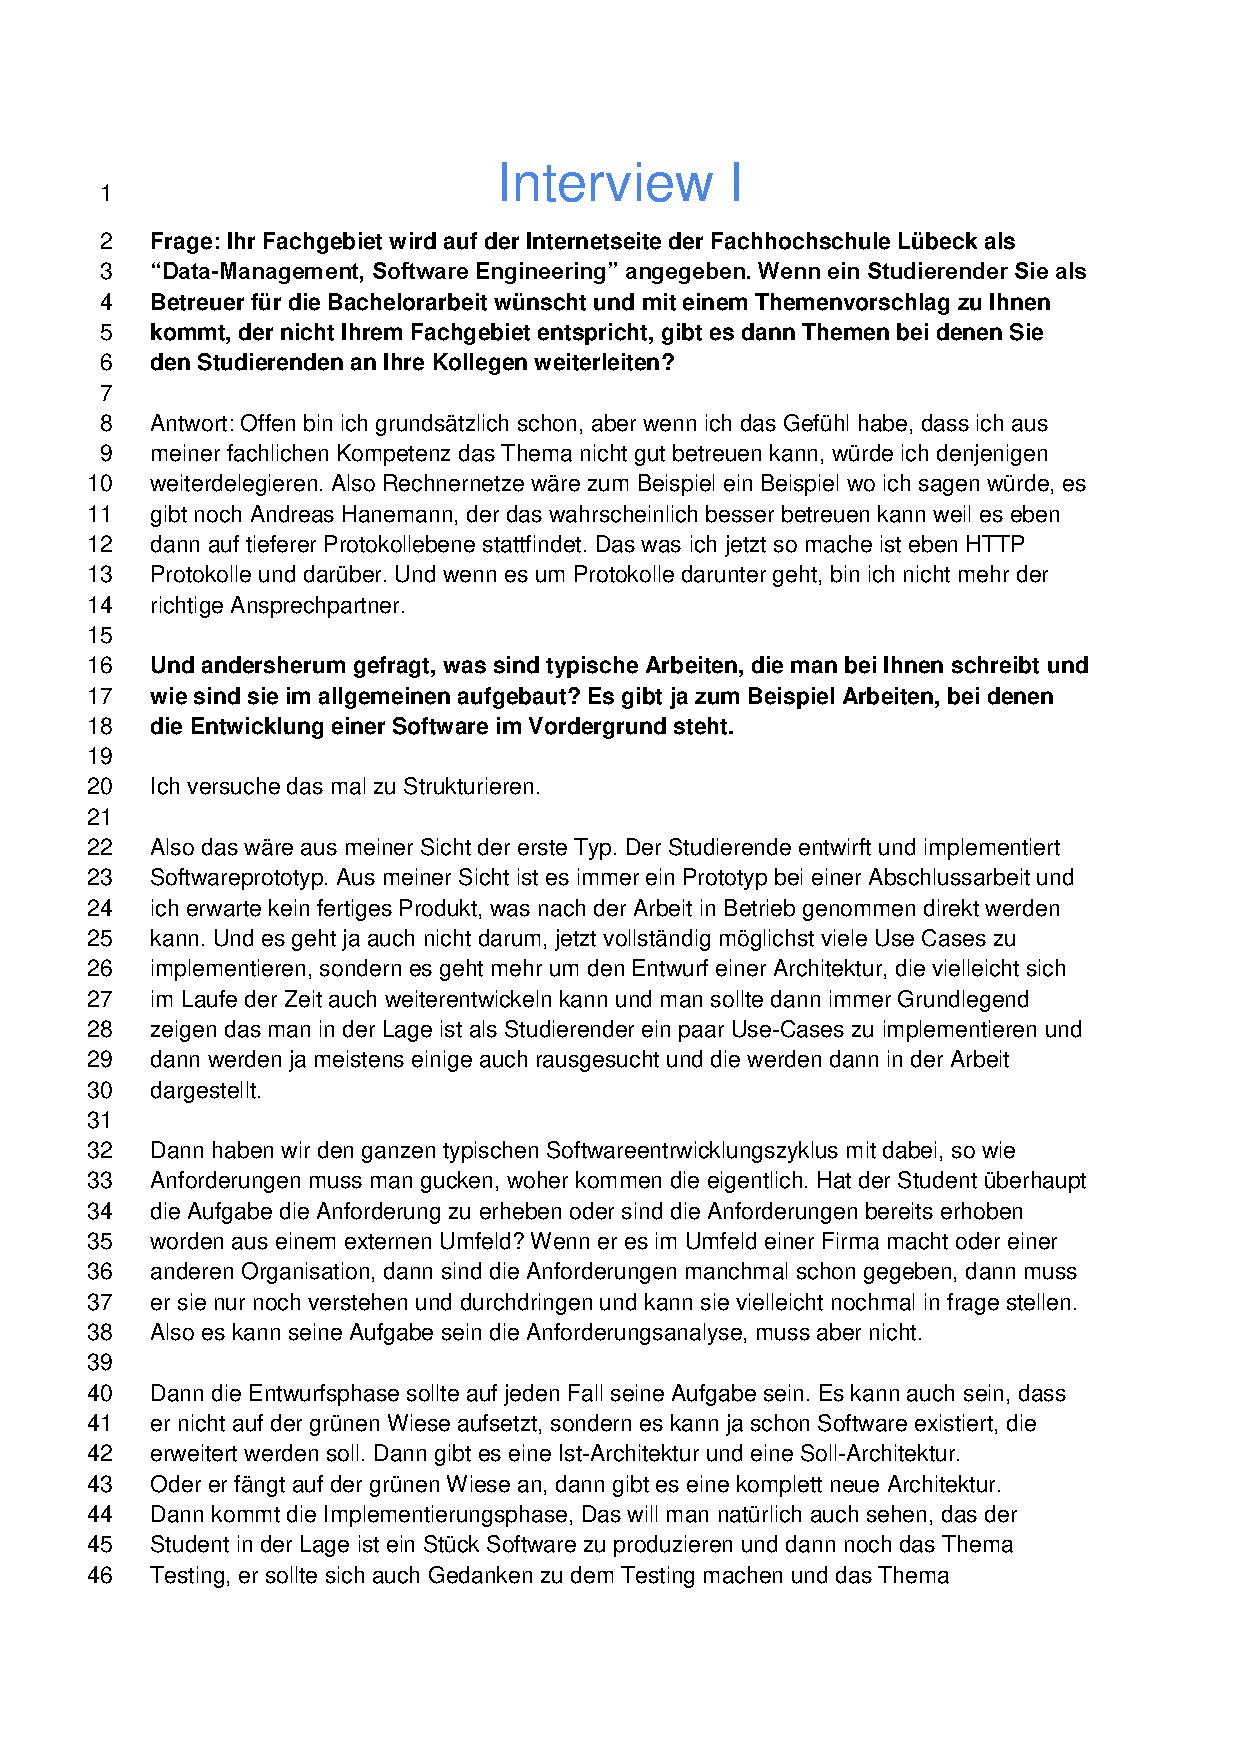
\includepdf[pages=-]{Anhang/Anforderungsanalyse/Professoren/Persoenliche_Interviews/Aufzeichnungen/Interview_I.pdf}

\includepdf[pages=-]{Anhang/Anforderungsanalyse/Professoren/Persoenliche_Interviews/Aufzeichnungen/Interview_II.pdf}

\includepdf[pages=-]{Anhang/Anforderungsanalyse/Professoren/Persoenliche_Interviews/Aufzeichnungen/Interview_III.pdf}
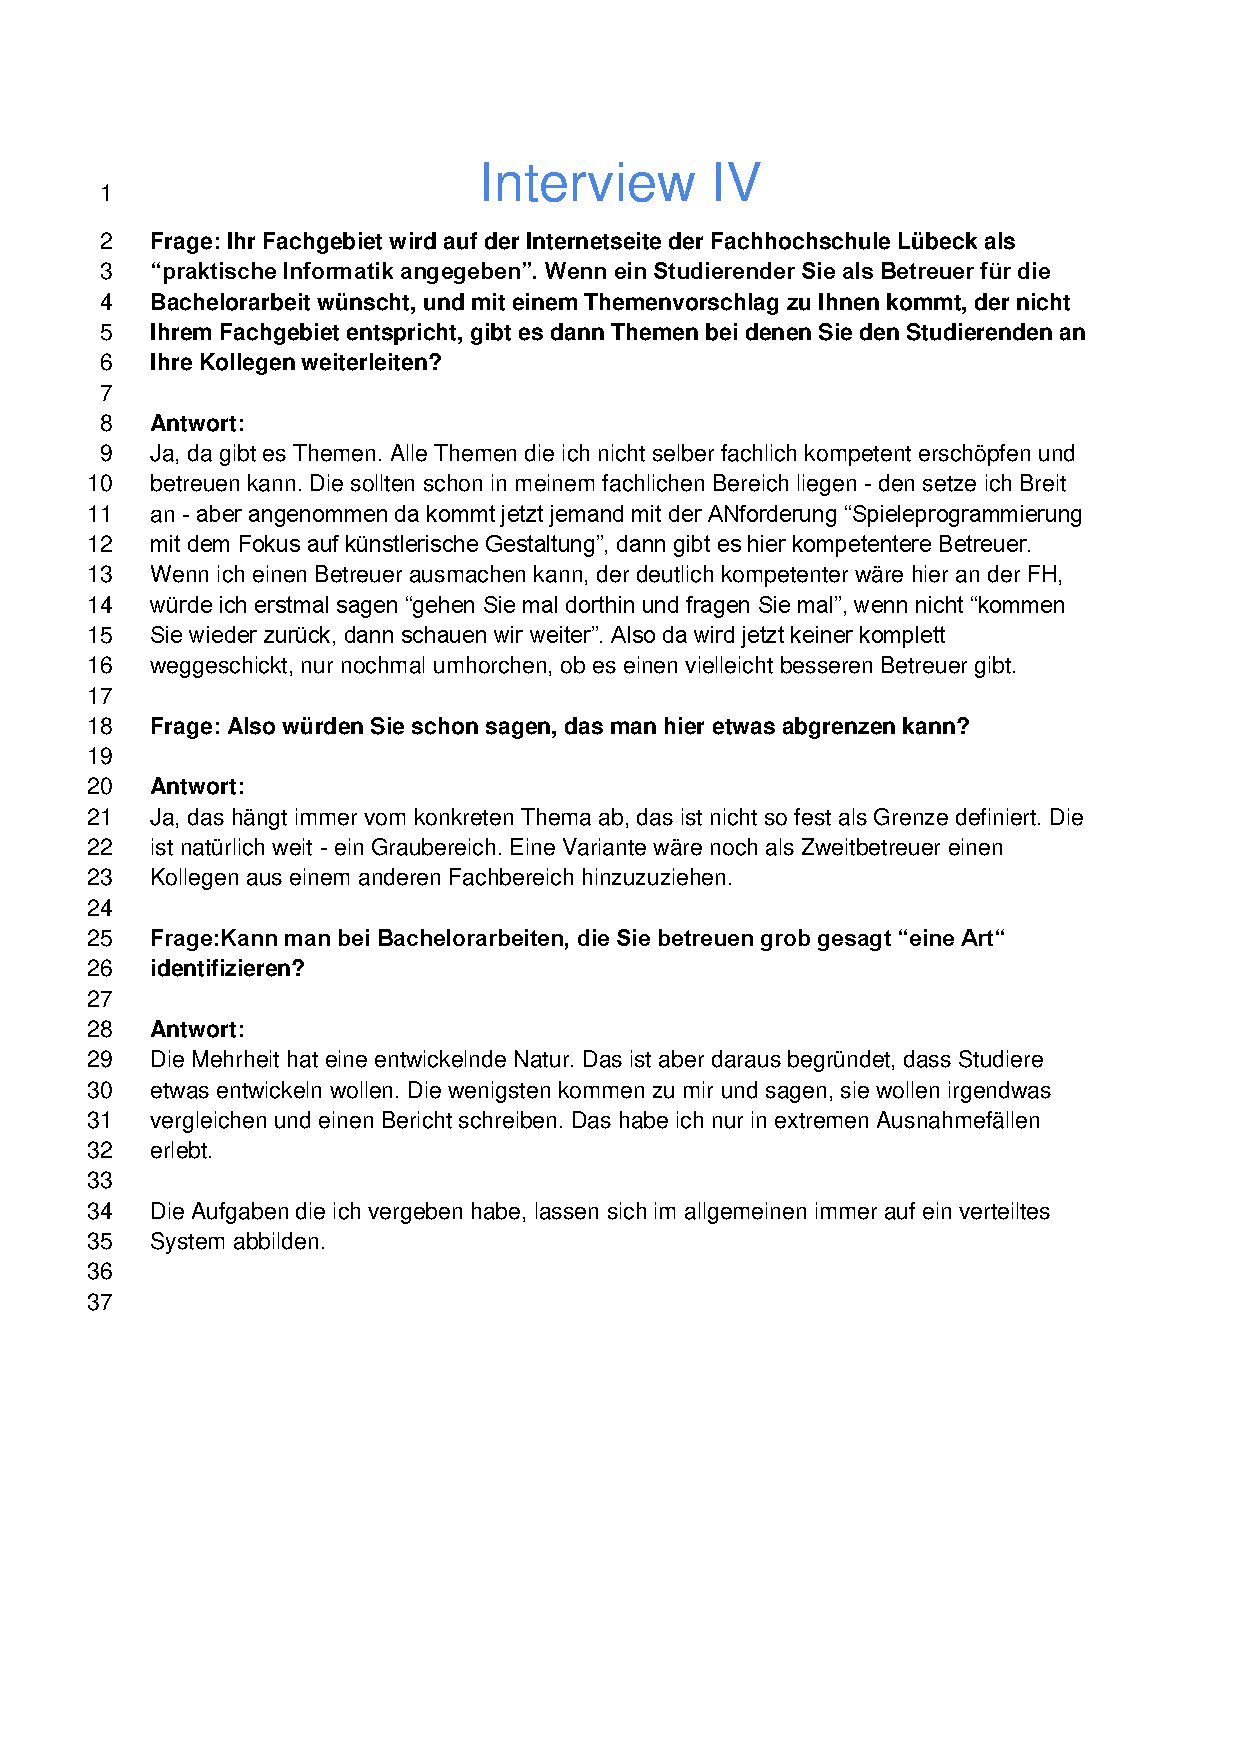
\includepdf[pages=-]{Anhang/Anforderungsanalyse/Professoren/Persoenliche_Interviews/Aufzeichnungen/Interview_IV.pdf}
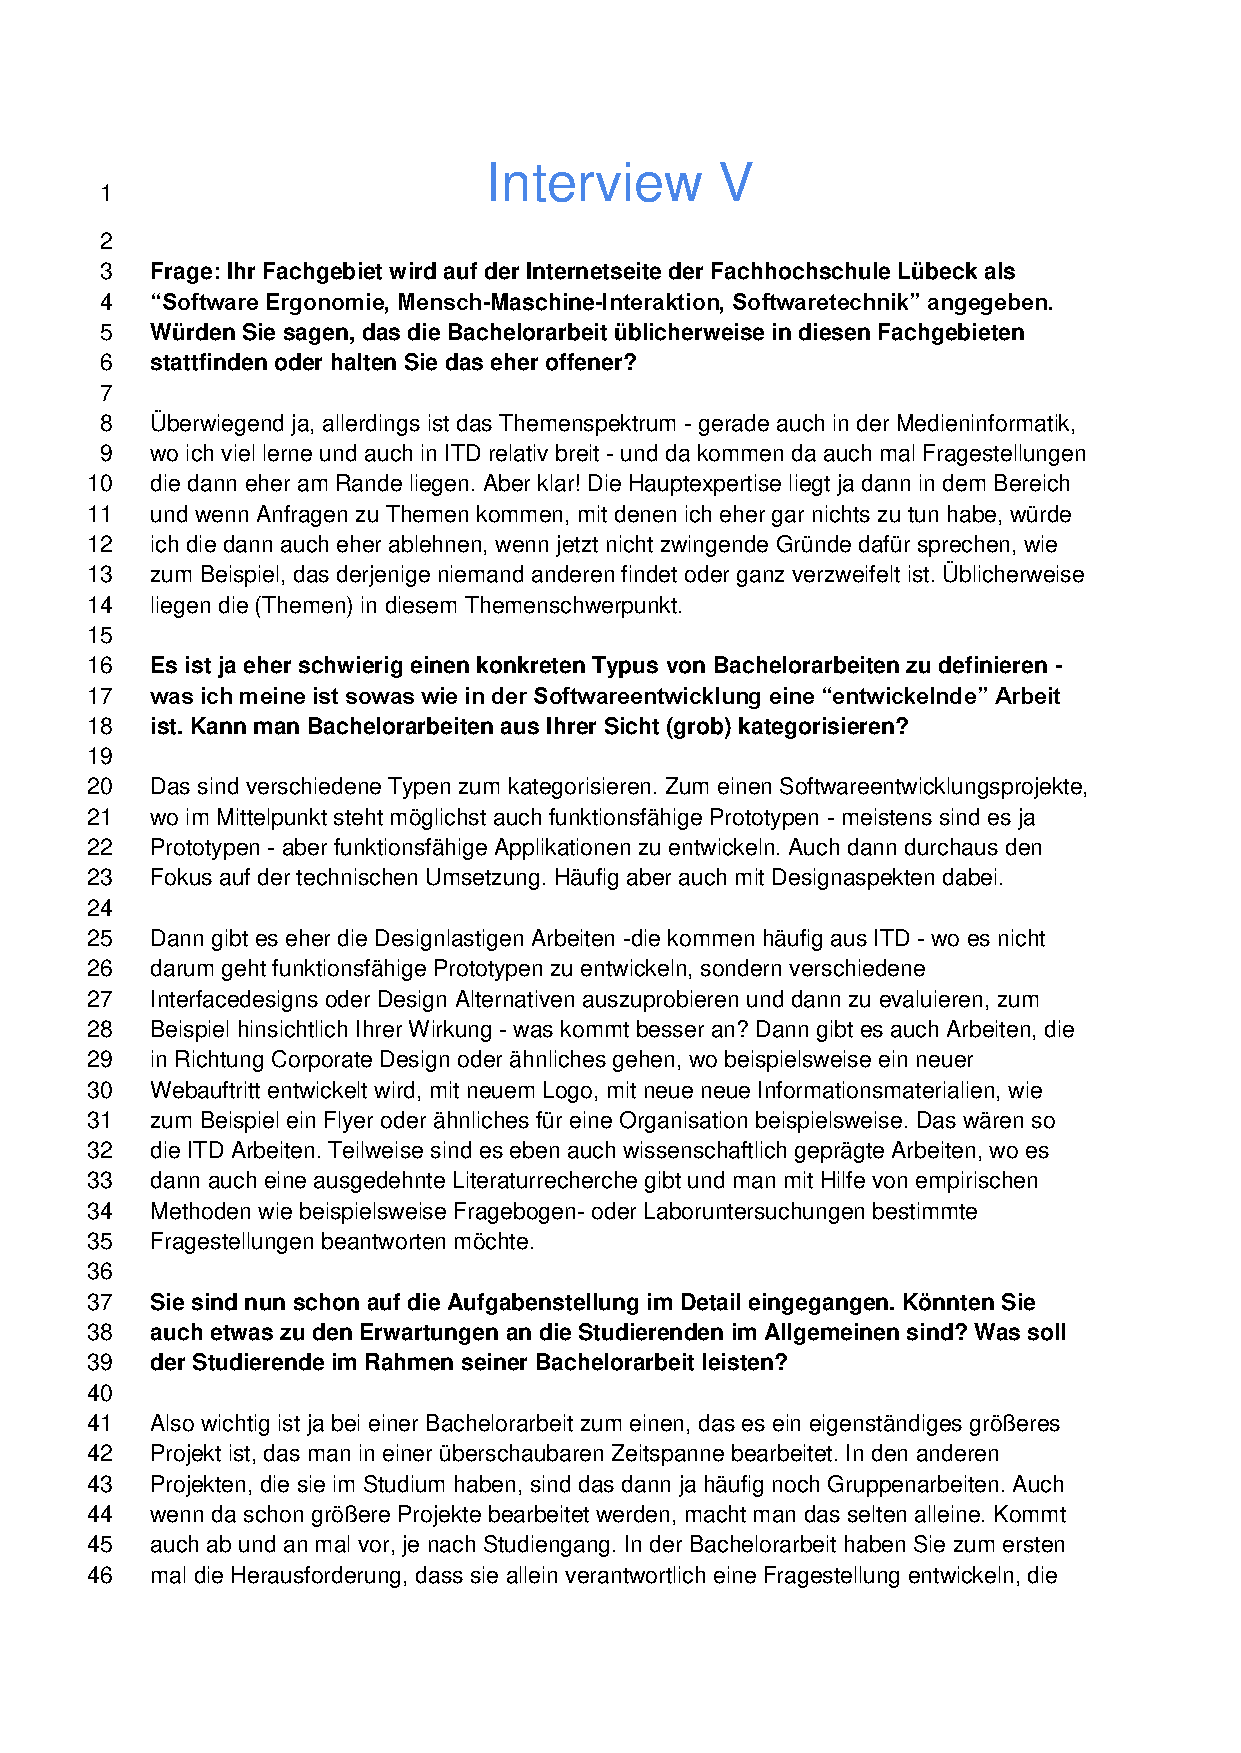
\includepdf[pages=-]{Anhang/Anforderungsanalyse/Professoren/Persoenliche_Interviews/Aufzeichnungen/Interview_V.pdf}

\newpage
\subsection{Zusammenfassung der schriftlichen Befragung der Studierenden}
\label{anhang:schriftlicheBefragungStudierendeZusammenfassung}
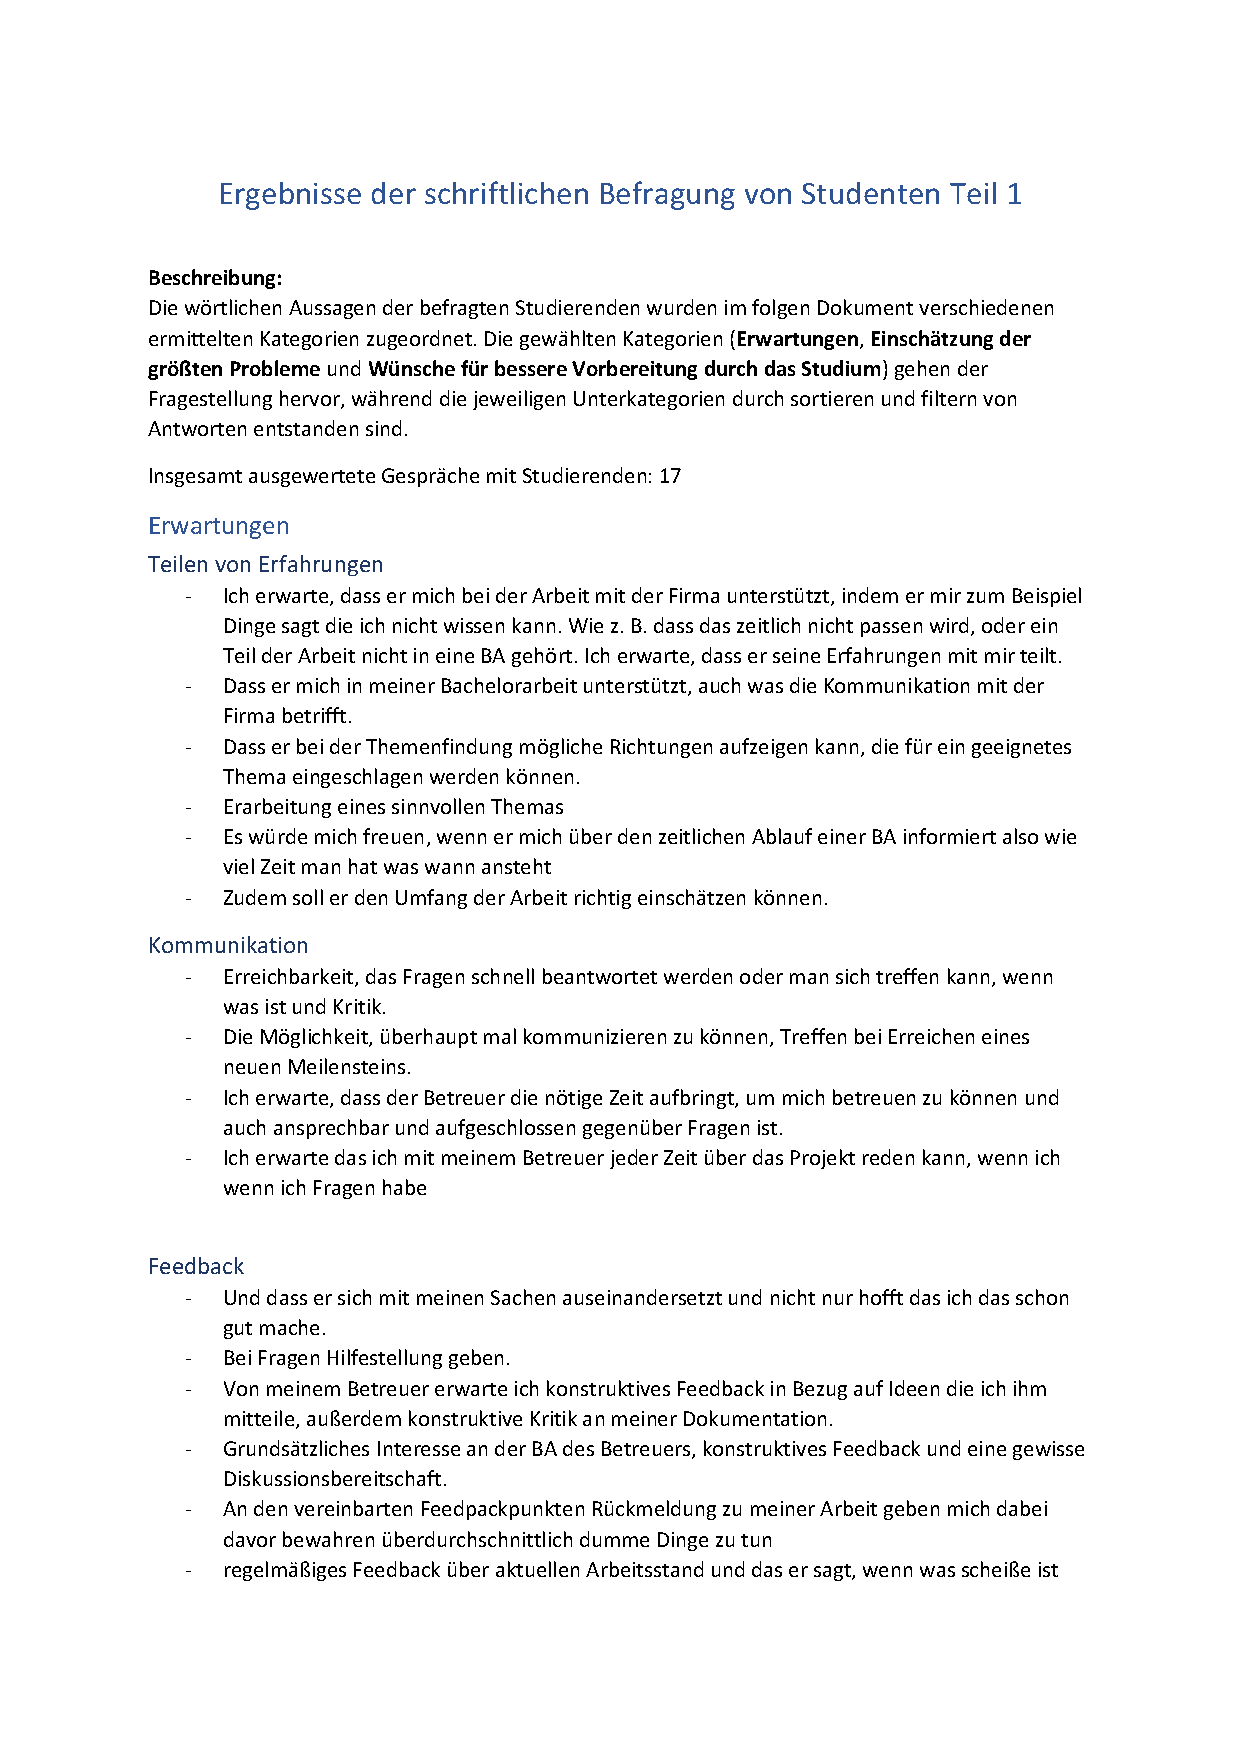
\includepdf[pages=-]{Anhang/Anforderungsanalyse/Studenten/Schriftliche_Befragung/Ergebnisse_der_Befragung.pdf}

\newpage
\subsection{Ergebnisse der Online-Umfrage für die Studierenden}
\label{anhang:onlineUmfrageStudierendeErgebnisse}
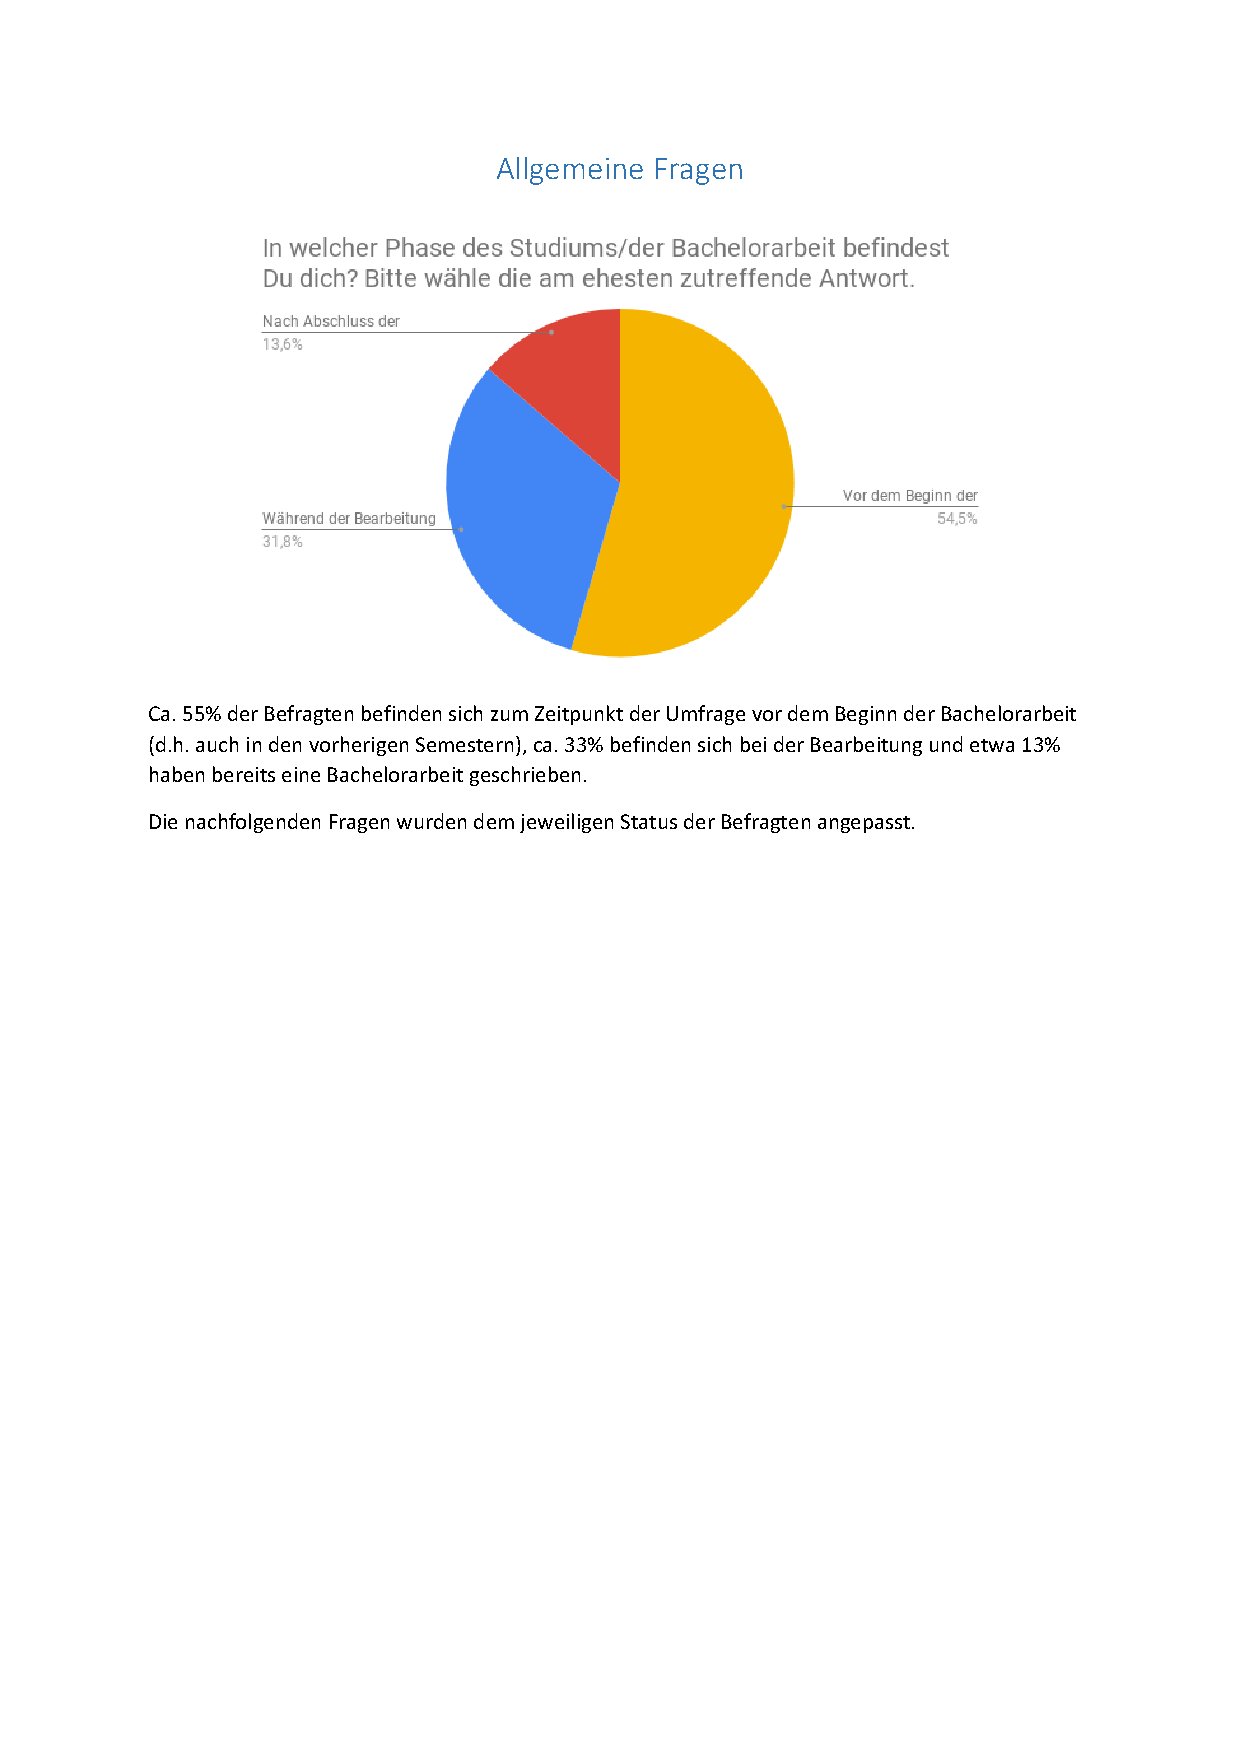
\includepdf[pages=-]{Anhang/Anforderungsanalyse/Studenten/Umfrage/Auswertung_Umfrage.pdf}


\nocite{*}
\printbibliography
\end{document}
